\documentclass[a4paper]{article}
\usepackage[T1]{fontenc}			% pacchetto per \chapter
\usepackage[italian]{babel}
\usepackage[italian]{isodate}  		% formato delle date in italiano
\usepackage{graphicx}				% gestione delle immagini
\usepackage{amsfonts}
\usepackage{booktabs}				% tabelle di qualità superiore
\usepackage{amsmath}				% pacchetto matematica
\usepackage{enumitem}				% gestione delle liste
\usepackage{pifont}					% pacchetto con elenchi carini
\usepackage{listings}				% pacchetto per i codici
\usepackage[x11names]{xcolor}		% pacchetto colori RGB
% Link ipertestuali per l'indice
\usepackage{xcolor}
\usepackage[linkcolor=black, citecolor=blue, urlcolor=cyan]{hyperref}
\hypersetup{
	colorlinks=true
}

\usepackage{fancyhdr}

% Intestazione e piè di pagina
% \pagestyle{fancy}
% \fancyhf{}
% \fancyhead[LE,RO]{\thepage}
% \fancyhead[RE]{\textit{\nouppercase{\leftmark}}}
% \fancyhead[LO]{\textit{\nouppercase{\rightmark}}}
% \renewcommand{\headrulewidth}{0.5pt}
% \renewcommand{\footrulewidth}{0pt}

\newcommand{\longline}{\noindent\rule{\textwidth}{0.4pt}}

\definecolor{codegreen}{rgb}{0,0.6,0}
\definecolor{codegray}{rgb}{0.5,0.5,0.5}
\definecolor{codepurple}{rgb}{0.58,0,0.82}
\definecolor{backcolour}{rgb}{0.95,0.95,0.92}
\lstdefinestyle{mystyle}{
	backgroundcolor=\color{backcolour},   
	commentstyle=\color{codegreen},
	keywordstyle=\color{magenta},
	numberstyle=\tiny\color{codegray},
	stringstyle=\color{codepurple},
	basicstyle=\ttfamily\footnotesize,
	breakatwhitespace=false,         
	breaklines=true,                 
	captionpos=b,                    
	keepspaces=true,                 
	numbers=left,                    
	numbersep=5pt,                  
	showspaces=false,                
	showstringspaces=false,
	showtabs=false,                  
	tabsize=2
}

\lstdefinelanguage{JavaScript}{
	keywords={typeof, new, true, false, catch, function, return, null, catch, switch, var, if, in, while, do, else, case, break},
	keywordstyle=\color{blue}\bfseries,
	ndkeywords={class, export, boolean, throw, implements, import, this},
	ndkeywordstyle=\color{darkgray}\bfseries,
	identifierstyle=\color{black},
	sensitive=false,
	comment=[l]{//},
	morecomment=[s]{/*}{*/},
	commentstyle=\color{codegreen}\ttfamily,
	stringstyle=\color{red}\ttfamily,
	morestring=[b]',
	morestring=[b]"
}

\lstset{
	language=JavaScript,
	backgroundcolor=\color{lightgray},
	extendedchars=true,
	basicstyle=\footnotesize\ttfamily,
	showstringspaces=false,
	showspaces=false,
	numbers=left,
	numberstyle=\footnotesize,
	numbersep=9pt,
	tabsize=2,
	breaklines=true,
	showtabs=false,
	captionpos=b
}

\lstset{style=mystyle}

%\usepackage{showframe}				% visualizzazione bordi
%\usepackage{showkeys}				% visualizzazione etichetta

\newcommand{\dquotes}[1]{``#1''}

\begin{document}
	\author{VR443470}
	\title{Programmazione e sicurezza delle reti}
	\date{\printdayoff\today}
	\maketitle
	
	\newpage
	
	% indice
	\tableofcontents
	
	\newpage
	
	\section{Scrittura di applicazioni di rete mediante interfaccia socket}
	
	\subsection{Host, processo e applicazione}
	
	L'\textcolor{Red3}{\textbf{host}} (colui che ospita) è una \textbf{macchina} sempre identificata da un indirizzo IP a cui, opzionalmente, può essere associato un nome Internet.\newline
	
	\noindent
	Il \textcolor{Red3}{\textbf{processo}} è un \textbf{programma in esecuzione} sull'host, il quale trasmette/riceve pacchetti verso/da altri processi su altri host attraverso la rete. Viene identificato tramite un numero di porta nell'intervallo $0$ - $65535$.\newline
	
	\noindent
	Un \textcolor{Red3}{\textbf{applicazione}} è una collaborazione tra un \textbf{insieme di processi} sparsi sulla rete per fare qualcosa di utile per l'utente, per esempio chat, e-mail, ecc.\newline
	
	\noindent
	Alcuni \textcolor{Green4}{\textbf{esempi}}:
	\begin{itemize}
		\item Eseguendo una ricerca su internet:
		\begin{itemize}
			\item Il \emph{web} è l'applicazione;
			\item Mentre i browser (Chrome, Firefox, Edge, Safari) sono il processo di esecuzione;
			\item L'host è il PC, tablet o smartphone su cui viene aperto il browser;
			\item Apache o NGINX è il processo di esecuzione sulla macchina remota, anch'essa identificata come host.
		\end{itemize}
		
		\item Aprendo un'applicazione come Telegram:
		\begin{itemize}
			\item Telegram è l'applicazione;
			\item Il processo di esecuzione è sempre l'app Telegram che è in esecuzione sul dispositivo attualmente in uso (PC, tablet, ecc.) che funge da host;
			\item Il server di Telegram è il processo di esecuzione sulla macchina remota, anch'essa identificata come host.
		\end{itemize}
	\end{itemize}\newpage

	\subsection{Modalità di trasmissione in Internet}
	
	Su Internet la modalità di trasmissione è una sequenza di byte chiamata: pacchetto, Protocol Data Unit (PDU), Datagram. A seconda del livello del protocollo, ci sono nomi diversi.
	
	\longline
	
	\subsubsection{Applicazioni orientate al datagramma (UDP)}
	
	Alcune \textbf{applicazioni sono orientate al datagramma}, quindi \textbf{ogni pacchetto scambiato tra gli host è indipendente dai precedenti e successivi}. Le \textbf{perdite} di pacchetti non vengono tenute in considerazione ed un \textcolor{Green4}{\textbf{esempio}} può essere la \textbf{trasmissione di temperature}: il ricevitore può non tener conto di alcune perdite poiché le informazioni ricevute non sono necessarie per il futuro.
	
	\longline
	
	\subsubsection{Applicazioni orientate alla connessione (TCP)}
	
	Invece, alcune \textbf{applicazioni sono orientate alla connessione}. A differenza delle applicazioni orientate al datagramma, quelle orientate alla connessione devono tener conto delle perdite poiché solitamente le informazioni scambiate sono di dimensioni rilevanti (e.g. un'immagine). Di conseguenza, una perdita provocherebbe una lettura parziale o impossibile da parte del ricevitore.\newline
	
	\noindent
	Il \textbf{socket} si preoccupa di \textbf{numerare i pacchetti appartenenti alla stessa connessione} per rilevare eventuali pacchetti persi e poterli ritrasmettere.\newline
	
	\noindent
	Il sistema operativo introduce all'interno dei pacchetti un numero di sequenza così che possa rilevare eventuali pacchetti persi e ritrasmetterli.
	\begin{itemize}
		\item \textcolor{Green4}{\textbf{Vantaggi:}}
		\begin{itemize}
			\item L'utente scrive/legge su un archivio remoto con la stessa naturalezza di quando scrive/legge su un archivio locale come se la rete in mezzo non ci fosse.
		\end{itemize}
		
		\item \textcolor{Red3}{\textbf{Svantaggi:}}
		\begin{itemize}
			\item Gli host mittente e destinatario eseguono un lavoro più complesso con il sistema operativo;
			\item Ritardo di ritrasmissione nel caso in cui i pacchetti vengano persi.
		\end{itemize}
	\end{itemize}\newpage

	\subsection{Schemi di applicazioni che utilizzano la rete}
	
	Le applicazioni di rete sono insiemi di processi su host diversi che si scambiano messaggi attraverso la rete. \textbf{Esistono degli schemi base che regolano lo scambio di messaggi}:
	\begin{itemize}
		\item Modello client/server;
		\item Modello Publisher/Subscriber (Pub/Sub)
	\end{itemize}

	\longline
	
	\subsubsection{Modello client/server}
	
	Il \textcolor{Red3}{\textbf{modello client/server}} è quello più utilizzato e funziona nel seguente modo (attenzione all'ordine!):
	\begin{enumerate}
		\item Il \emph{client} esegue una \textbf{richiesta} inviando dei dati al \emph{server};
		
		\item Il \emph{server} riceve i dati del \emph{client}, processa i dati e invia la \textbf{risposta} al \emph{client}. Infine, si mette in attesa di altre richieste.
	\end{enumerate}
	I dati inviati dal \emph{client} possono essere delle trasmissioni di dati o delle richieste di dati. In ogni caso, \textbf{il ruolo è determinato dall'ordine dei messaggi e non dal contenuto}. Si noti che il \emph{client} e \emph{server} \textbf{sono processi e \underline{non host}}. Infatti, l'insieme di un client e un server costituisce l'applicazione di rete.\newline
	
	\noindent
	Un \textcolor{Green4}{\textbf{esempio}} di applicazione client/server è il \textbf{sensore di temperatura corporea} che funge da client e invia al server una temperatura. Le risposte del server sono \dquotes{OK} per confermare l'avvenuta ricezione.\newline
	
	\noindent
	Un altro \textcolor{Green4}{\textbf{esempio}} di applicazione client/server è il display che funge da cliente e chiede al server una temperatura. Le risposte del server in questo caso saranno i dati richiesti.
	
	\longline
	
	\subsection{Creazione dell'interfaccia Socket}
	
	Il programma, prima di utilizzare la rete, deve essere in grado di creare un oggetto di tipo \textbf{socket}. Esso è identificato principalmente da tre parametri:
	\begin{itemize}
		\item Indirizzo IP locale;
		
		\item Porta locale, la quale è un intero senza segno di 16 bit (quindi da 0 a 65'535). Nel modello client/server:
		\begin{itemize}
			\item Il \textbf{server} deve decidere esplicitamente il numero di porta affinché i client possano saperlo (da 0 a 1023 le porte sono chiamate \dquotes{porte note} perché sono utilizzate per protocolli famosi come HTTP);
			
			\item Il \textbf{client} può decidere se scegliere il numero di porta esplicitamente oppure delegare la scelta al sistema operativo.
		\end{itemize}

		\item Modalità di trasmissione: UDP o TCP.
	\end{itemize}\newpage
	
	\subsection[\textcolor{Green4}{\textbf{Esempi}} di codice]{Esempi di codice}
	
	\subsubsection{Esecuzione degli esempi}
	
	\begin{enumerate}
		\item Aprire due terminali
		
		\item Compilare il server e successivamente eseguirlo con il comando:
		\begin{lstlisting}[language=C]
			-gcc network.c serverUDP.c -o serverUDP -lpthread\end{lstlisting}
		
		\item Compilare il client e successivamente eseguirlo con il comando:
		\begin{lstlisting}[language=C]
			-gcc network.c clientUDP.c -o clientUDP -lpthread\end{lstlisting}
	\end{enumerate}

	\longline
	
	\subsubsection{Client UDP}\label{client UDP}
	
	Il client UDP ha il seguente codice:
	\lstinputlisting[language=C]{code/clientUDP.c}
	\begin{itemize}
		\item (4-8) dichiarazione delle variabili tra cui la variabile socket;
	
		\item (10) inizializzazione dell'interfaccia socket sulla porta 20'000;
	
		\item (13) invio, tramite UDP, il messaggio \dquotes{Ciao sono il client!} al destinatario avente indirizzo IP \dquotes{127.0.0.1} (\emph{localhost}) e porta 35'000;
	
		\item (14) attesta dell'arrivo della risposta del server;
		
		\item (15-16) scrittura sul terminale della porta, dell'indirizzo del mittente e del messaggio.
	\end{itemize}\newpage
	
	\subsubsection{Server UDP}\label{server UDP}
	
	Il server UDP ha il seguente codice:
	\lstinputlisting[language=C]{code/serverUDP.c}
	\begin{itemize}
		\item (4-8) dichiarazione delle variabili tra cui la variabile socket;
		
		\item (10) inizializzazione dell'interfaccia socket sulla porta 35'000;
		
		\item (12) attesta dell'arrivo di qualche messaggio da parte di qualche client;
		
		\item (13-14) ricezione di un messaggio da parte di un client e stampa sul terminale dell'indirizzo, della porta e del messaggio del mittente;
		
		\item (15) invio della risposta del server al client.
	\end{itemize}\newpage

	\subsubsection{Client\_inc UDP}\label{client_inc UDP}
	
	Il client UDP (paragrafo~\ref{client UDP}) può essere riscritto nel seguente modo:
	\lstinputlisting[language=C]{code/clientUDP_inc.c}
	\begin{itemize}
		\item (4-8) dichiarazione delle variabili tra cui la variabile socket;
		
		\item (10) inizializzazione dell'interfaccia socket sulla porta 20'000;
		
		\item (11-12) inserimento di un numero intero da parte dell'utente;
		
		\item (13) invio, tramite UDP, del numero inserito dall'utente al destinatario avente indirizzo IP \dquotes{127.0.0.1} (\emph{localhost}) e porta 35'000;
		
		\item (14) attesta dell'arrivo della risposta del server;
		
		\item (15-16) scrittura sul terminale della porta, dell'indirizzo del mittente e del messaggio.
	\end{itemize}\newpage

	\subsubsection{Server\_inc UDP}\label{server_inc UDP}
	
	Il server UDP (paragrafo~\ref{server UDP}) può essere riscritto nel seguente modo:
	\lstinputlisting[language=C]{code/serverUDP_inc.c}
	\begin{itemize}
		\item (4-8) dichiarazione delle variabili tra cui la variabile socket;
		
		\item (10) inizializzazione dell'interfaccia socket sulla porta 35'000;
		
		\item (12) attesta dell'arrivo di qualche messaggio da parte di qualche client;
		
		\item (13-14) ricezione di un messaggio da parte di un client e stampa sul terminale dell'indirizzo, della porta e del messaggio del mittente;
		
		\item (15) incremento di uno del valore intero ottenuto;
		
		\item (15) invio della risposta del server al client con il valore incrementato.
	\end{itemize}\newpage

	\subsubsection{Client TCP}\label{client TCP}
	
	Il client TCP ha il seguente codice:
	\lstinputlisting[language=C]{code/clientTCP.c}
	\begin{itemize}
		\item (4-5) dichiarazione delle variabili tra cui la variabile \textsf{connection} per gestire la connessione;
		
		\item (7-8) creazione di una connessione TCP con il server utilizzando \emph{localhost} e la porta 35'000. 
		
		\item (9-10) controllo del valore della connessione per verificare se c'è stato un errore. In tal caso, la connessione termina con la stampa dell'errore su terminale;
		
		\item (12-15) in caso di connessione riuscita, il client richiede l'inserimento di un valore intero all'utente;
		
		\item (16-17) invio del valore intero al server;
		
		\item (18) attesa di una risposta da parte del server;
		
		\item (19-20) al momento della ricezione della risposta, il client stampa la risposta del server e chiude la connessione.
	\end{itemize}\newpage
	
	\subsubsection{Server TCP}\label{server TCP}
	
	Il server TCP ha il seguente codice:
	\lstinputlisting[language=C]{code/serverTCP.c}
	\begin{itemize}
		\item (4-6) dichiarazione delle variabili tra cui la variabile \textsf{connection} per gestire la connessione e \textsf{socket} per gestire i dati;
		
		\item (8) inizializzazione di un socket TCP utilizzando la porta 35'000.
		
		\item (9-10) controllo del valore del socket per verificare se c'è stato un errore. In tal caso, la creazione termina con la stampa dell'errore su terminale;
		
		\item (12-14) in caso di creazione del socket riuscita, il server attende la connessione da parte di qualche client;
		
		\item (15-17) attesa di una richiesta da parte di qualche client. Nel momento in cui viene ricevuta una richiesta, il server la accetta e instaura la connessione e attende la ricezione dei dati;
		
		\item (18-19) all'arrivo dei dati da parte del client, il server esegue un incremento di uno del valore ricevuto dal client;
		
		\item (20-22) il server invia il valore al client e infine chiude la connessione.
	\end{itemize}\newpage

	\subsubsection{Codice per la copia di un file}
	
	Il codice per la copia di un file è strutturato nel seguente modo:
	\lstinputlisting[language=C]{code/fileCopy.c}
	\begin{itemize}
		\item (6-29) dichiarazione dei puntatori ai file e tentativi di apertura dei due file richiesti dall'utente;
		
		\item (32-37) viene eseguita la lettura dal primo file e salvata nella variabile \textsf{c}. A questo punto, finché viene letto un carattere valido, ovvero che non sia la fine del file (\emph{End Of File}, EOF), il contenuto della variabile \textsf{c} viene inserito nel secondo file;

		\item (39-43) al termine del processo di copia, viene stampato il file nel quale sono stati copiati i valori e chiusi i rispettivi file descriptors.
	\end{itemize}\newpage
	
	\subsection[\textcolor{Red3}{\textbf{Esercizi}}]{Esercizi}
	
	\subsubsection{Esercizio 1 - UDP}
	
	Lanciare prima il server e poi il client. Cosa si osserva? Invertire la sequenza di lancio. Cosa si osserva?\newline
	
	\noindent
	\textcolor{Green4}{\textbf{\emph{\underline{Soluzione}}}}\newline
	
	\noindent
	Lanciando il server e successivamente il client, il primo attende la connessione da parte di qualcuno. Quindi, una volta avviato il client, le due parti inizieranno a comunicare.
	
	Invece, avviando prima il client e successivamente il server, le due parti non riescono a comunicare. Questo perché il client tenta di raggiungere un host non esistente.
	
	\longline
	
	\subsubsection{Esercizio 2 - UDP}
	
	Modificare i sorgenti per consentire al server di ricevere sulla porta 10000 e il client di trasmettere sulla propria porta 30000 (ogni modifica dei sorgenti richiede una loro ricompilazione).\newline
	
	\noindent
	\textcolor{Green4}{\textbf{\emph{\underline{Soluzione}}}}\newline
	
	\noindent
	Le modifiche da effettuare sono banali, ecco qua di seguito i codici del client (spiegazione al paragrafo~\ref{client UDP}):
	\lstinputlisting[language=C]{code/clientUDP_mod2.c}\newpage
	
	\noindent
	E del server (spiegazione al paragrafo~\ref{server UDP}):
	\lstinputlisting[language=C]{code/serverUDP_mod2.c}
	
	\longline
	
	\subsubsection{Esercizio 3 - UDP}
	
	Mettere il server in ascolto sulla porta 100 e osservare cosa succede:
	\begin{itemize}
		\item Bisogna modificare anche il client? Se sì, dove?
		\item Per chi usa il proprio PC con Linux o una virtual machine Linux, lanciare il server con il comando \dquotes{\textsf{sudo ./serverUDP}} e osservare cosa cambia.
	\end{itemize}

	\noindent
	\textcolor{Green4}{\textbf{\emph{\underline{Soluzione}}}}\newline
	
	\noindent
	Modificando il codice e inserendo il numero di porta 100, il server non riesce ad essere eseguito per un problema della porta. Infatti, la porta 100 fa parte delle \emph{well-know port} e non può essere utilizzata per altri scopi.\newline
	
	\noindent
	Modificando anche il client e inviando il messaggio al localhost con porta 100, il codice viene compilato ed eseguito correttamente. Ovviamente il client rimane in attesa del server.\newline
	
	\noindent
	Compilando il server con la modalità \textsf{sudo} è possibile forzare la modifica della porta 100 e mettersi in ascolto su tale porta. Di conseguenza, il server si metterà in ascolto sulla porta 100 e il client che eseguirà l'invio di un messaggio in tale porta, riuscirà a trasmettere il messaggio.\newpage
	
	\subsubsection{Esercizio 4 - UDP}
	
	Sostituire \dquotes{127.0.0.1} (o la stringa \dquotes{localhost}) con localhost (o al contrario con 127.0.0.1) e poi con \dquotes{pippo} e osservare cosa succede.\newline
	
	\noindent
	\textcolor{Green4}{\textbf{\emph{\underline{Soluzione}}}}\newline
	
	\noindent
	Modificando il parametro della chiamata a funzione \textsf{UDPSend} nel client viene modificato l'indirizzo del destinatario:
	\begin{itemize}
		\item Inserendo \dquotes{127.0.0.1} si sta inserendo l'indirizzo privato creato per identificare l'host stesso;

		\item Inserendo \textsf{localhost} si sta utilizzando un \emph{alias}, dunque è come scrivere l'indirizzo \dquotes{127.0.0.1};

		\item Inserendo \dquotes{Pippo} si sta provando a identificare l'alias Pippo a qualche indirizzo. Purtroppo non esiste nessun alias all'interno del sistema operativo con tale valore, tuttavia su Linux (forse anche su Windows) è possibile creare alias di rete con il relativo indirizzo IP.
	\end{itemize}

	\longline
	
	\subsubsection{Esercizio 5 - UDP}
	
	(Da fare solo se in Lab Delta) Accordarsi per lavorare su coppie di macchine in modo che server e client siano su macchine diverse. Come bisogna modificare i sorgenti?\newline
	
	\noindent
	\textcolor{Green4}{\textbf{\emph{\underline{Soluzione}}}}\newline
	
	\noindent
	La modifica è alquanto semplice. Supponendo che i due host siano connessi sulla stessa rete, quindi non per forza la rete universitaria ma va bene anche un hotspot tramite telefono, è necessario modificare nel seguente modo i codici:
	\begin{itemize}
		\item Server: non apportare nessuna modifica in quanto il server (destinatario) deve solo aprire una porta, nel caso d'esempio la 35000;
		
		\item Client: indipendentemente dalla porta aperta nel client, di default nell'esempio la 20000, il client necessita di una modifica nei parametri della chiamata a funzione \textsf{UDPSend}. In particolare, al posto di \textsf{localhost} o dell'indirizzo \dquotes{127.0.0.1}, basterà inserire l'indirizzo IP del server che ha all'interno della rete. È doveroso cambiare anche il numero di porta nel caso in cui sia stata cambiata nel server.
		
		Attenzione, nelle virtual machine non è così semplice la faccenda. Infatti esse utilizzano un bridge per collegarsi alla scheda di rete e di conseguenza l'IP che viene visualizzato non è \dquotes{reale}. Si consiglia dunque un sistema operativo linux (o windows) non virtualizzato.
	\end{itemize}\newpage
	
	\subsubsection{Esercizio 6 - UDP}
	
	Modificare il server in maniera che soddisfi 5 richieste prima di terminare.
	\begin{itemize}
		\item E se volessi che non terminasse mai?
	\end{itemize}

	\noindent
	\textcolor{Green4}{\textbf{\emph{\underline{Soluzione}}}}\newline
	
	\noindent
	Per soddisfare almeno 5 richieste, è necessario modificare il codice del server di modo che esegua la parte di codice della ricezione almeno 5 volte. Quindi il relativo codice del server sarà:
	\lstinputlisting[language=C]{code/serverUDP_mod3.c}
	Mentre quello del client non viene modificato.
	
	\noindent
	La simulazione dell'esecuzione sarà la seguente (prossima pagina):
	\begin{figure}[!htp]
		\centering
		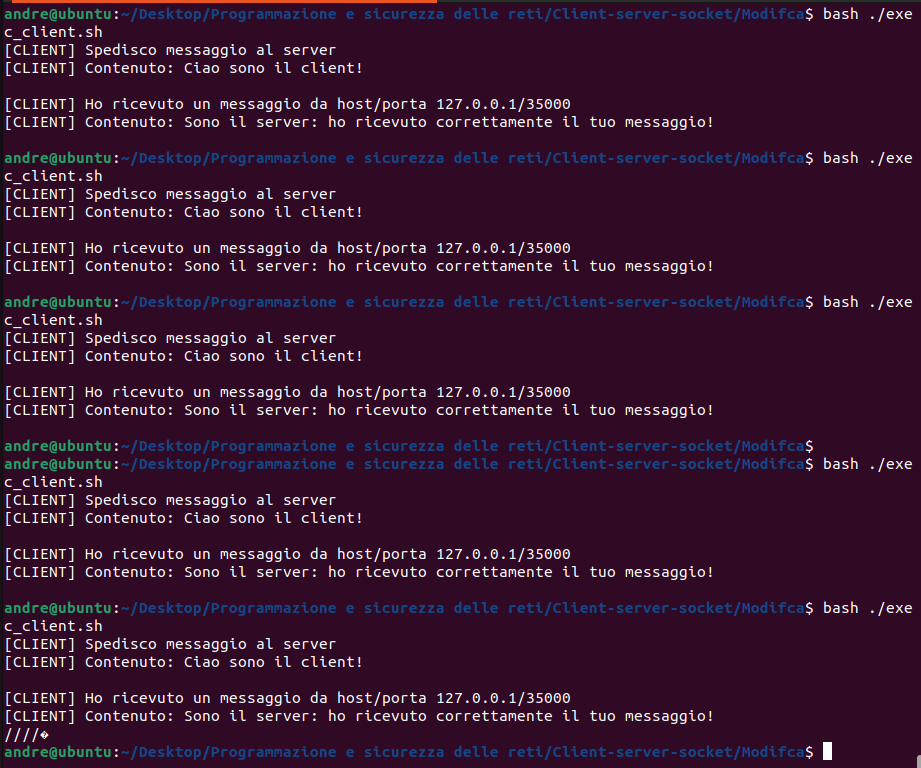
\includegraphics[width=\textwidth]{img/soluzioni_TCP-UDP/TCP-UDP_1.png}
		\caption{Terminale client.}
		\:\newline
		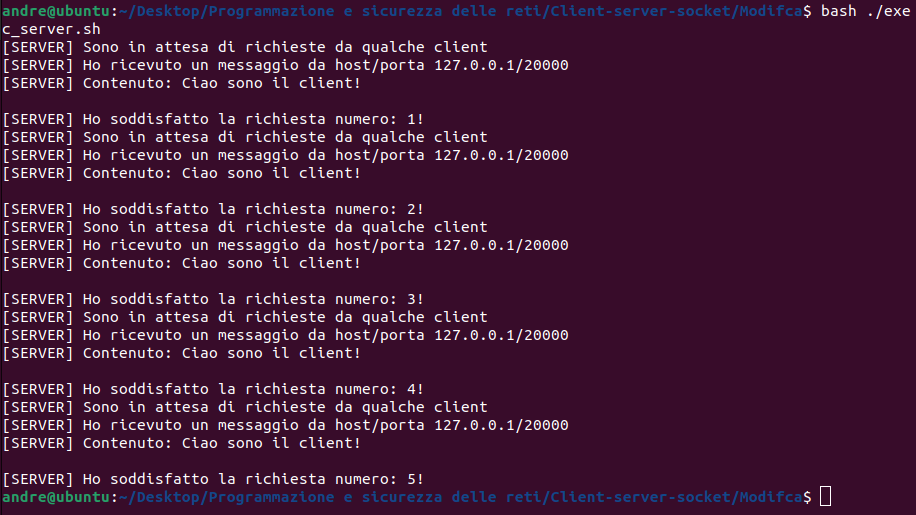
\includegraphics[width=\textwidth]{img/soluzioni_TCP-UDP/TCP-UDP_2.png}
		\caption{Terminale server.}
	\end{figure}\newpage

	\subsubsection{Esercizio 7 - UDP}
	
	Compilare ed eseguire il secondo esempio.\newline
	
	\noindent
	\textcolor{Green4}{\textbf{\emph{\underline{Soluzione}}}}\newline
	
	\noindent
	Si esegue il secondo esempio che riguarda il clientUDP e serverUDP in versione \_inc, rispettivamente paragrafo~\ref{client_inc UDP} e \ref{server_inc UDP}.
	
	\longline
	
	\subsubsection{Esercizio 8 - Sommatrice UDP}\label{esercizio 8 - Sommatrice UDP}
	
	Modificare il codice in modo tale da costruire una semplice sommatrice:
	\begin{itemize}
		\item Il client acquisisce ripetutamente da tastiera un numero intero e lo invia al server finché l'utente digita zero;
		
		\item Il server accumula in una variabile \dquotes{somma} i valori mandati dal client finché il client manda zero;
		
		\item Quando il client manda zero il server risponde al client con la somma ottenuta.
	\end{itemize}

	\noindent
	\textcolor{Green4}{\textbf{\emph{\underline{Soluzione}}}}\newline
	
	\noindent
	Il codice del client:
	\lstinputlisting[language=C]{code/clientUDP_inc_mod2.c}
	\begin{itemize}
		\item (11-16) Viene richiesto l'inserimento di un numero intero all'utente finché tale numero non è diverso da zero. Ogni numero viene inviato al server (15).
		
		\item (17-19) Nel momento in cui il numero inserito è zero, il programma termina aspettando il risultato che verrà inviato dal server. Alla ricezione, verrà stampato.
	\end{itemize}\newpage
	
	\noindent
	\begin{figure}[!htp]
		\centering
		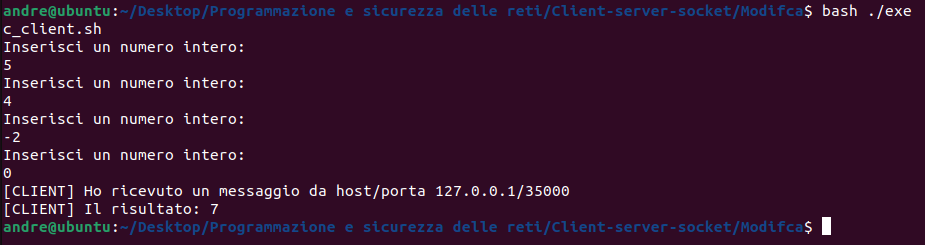
\includegraphics[width=\textwidth]{img/soluzioni_TCP-UDP/TCP-UDP_3.png}
		\caption{Esempio di esecuzione del client.}
	\end{figure}

	\noindent
	Il codice del server:
	\lstinputlisting[language=C]{code/serverUDP_inc_mod2.c}
	\begin{itemize}
		\item (12-19) Viene dichiarata la variabile somma, come richiesto dall'esercizio. Successivamente, il server attende che qualche client gli invii un valore intero. Una volta arrivato tale informazione, il server somma il valore ad una sua variabile locale. Il ciclo continua finché non riceve un valore pari a zero.
		
		\item (20-22) Quando viene ricevuto un valore pari a zero, il server invia la somma effettuata al client e stampa chi è il client che ha richiesto la terminazione.
	\end{itemize}\newpage

	\noindent
	\begin{figure}[!htp]
		\centering
		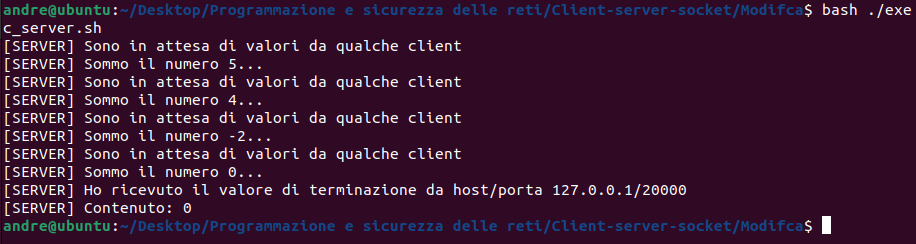
\includegraphics[width=\textwidth]{img/soluzioni_TCP-UDP/TCP-UDP_4.png}
		\caption{Esempio di esecuzione del server.}
	\end{figure}\newpage

	\subsubsection{Esercizio 9 - Sommatrice UDP e perdita di pacchetti}\label{esercizio 9 - Sommatrice UDP e perdita di pacchetti}
	
	Usare la sommatrice su due macchine distinte provando, sulla macchina del client, a staccare il cavo di rete prima di un invio di un dato, ad esempio:
	\begin{itemize}
		\item Digitare \dquotes{2345} + INVIO
		\item Digitare \dquotes{5187} + INVIO
		\item \textbf{Staccare il cavo}
		\item Digitare \dquotes{2} + INVIO
		\item \textbf{Riattaccare il cavo e aspettare 30 sec che il sistema operativo si riassesti}
		\item Digitare \dquotes{1} + INVIO
		\item \dquotes{0}
	\end{itemize}
	Che somma leggo? È corretta?\newline
	
	\noindent
	\textcolor{Green4}{\textbf{\emph{\underline{Soluzione}}}}\newline
	
	\noindent
	Si parte con il rispondere prima alla domanda e poi a fornire la motivazione. La somma letta \underline{non} è corretta. La motivazione è la seguente:
	\begin{itemize}
		\item Il client invia il valore 2345 al server. Quest'ultimo riceve correttamente il valore. Somma progressiva: $2345$;
		
		\item Il client invia il valore 5187 al server. Quest'ultimo riceve correttamente il valore. Somma progressiva: $2345 + 5187 = 7532$;
		
		\item Viene staccato il cavo;
		
		\item Inserimento del valore 2 all'interno del client. Quest'ultimo invia il pacchetto al localhost, il quale non è collegato alla rete, di conseguenza il pacchetto viene perso. Dato che il protocollo è UDP, il client non sa se il pacchetto è stato ricevuto dal destinatario oppure no, di conseguenza ricomincia il ciclo e richiede un numero intero. La somma nel server rimane $7532$, mentre la somma corretta dovrebbe essere $7532+2=7534$;
		
		\item Viene riattaccato il cavo;
		
		\item Il client invia il valore 1 al server. Quest'ultimo riceve correttamente il valore. Somma progressiva: $7532+1 = 7533$;
		
		\item Valore zero, il client e il server si fermano.
	\end{itemize}\newpage

	\subsubsection{Esercizio 10 - Sommatrice UDP e influenze reciproche}\label{esercizio 10 - Sommatrice UDP e influenze reciproche}
	
	Invocare il server della sommatrice con due client diversi (tutti e tre possono anche essere sulla stessa macchina ovviamente su finestre terminali diverse), ad esempio:
	\begin{table}[!htbp]
		\centering
		\begin{tabular}{@{} l | l @{}}
			\toprule
			\textbf{Client A} & \textbf{Client B} \\
			\midrule
			Digitare \dquotes{2345} + INVIO	& Digitare \dquotes{2} + INVIO 	\\
			Digitare \dquotes{5187} + INVIO	& Digitare \dquotes{8} + INVIO 	\\
			Digitare \dquotes{2} + INVIO	& \dquotes{0} 					\\
			Digitare \dquotes{1} + INVIO	& 								\\
			\dquotes{0}						&								\\
			\bottomrule
		\end{tabular}
	\end{table}
	
	\noindent
	Che somma leggo da ciascun client? È la somma che ciascun client si aspetterebbe?\newline
	
	\noindent
	\textcolor{Green4}{\textbf{\emph{\underline{Soluzione}}}}\newline
	
	\noindent
	Mantenendo lo schema dell'esercizio 8 (paragrafo~\ref{esercizio 8 - Sommatrice UDP}), l'esecuzione dei due client (A e B) come nello schema dell'esercizio:
	\begin{figure}[!htp]
		\centering
		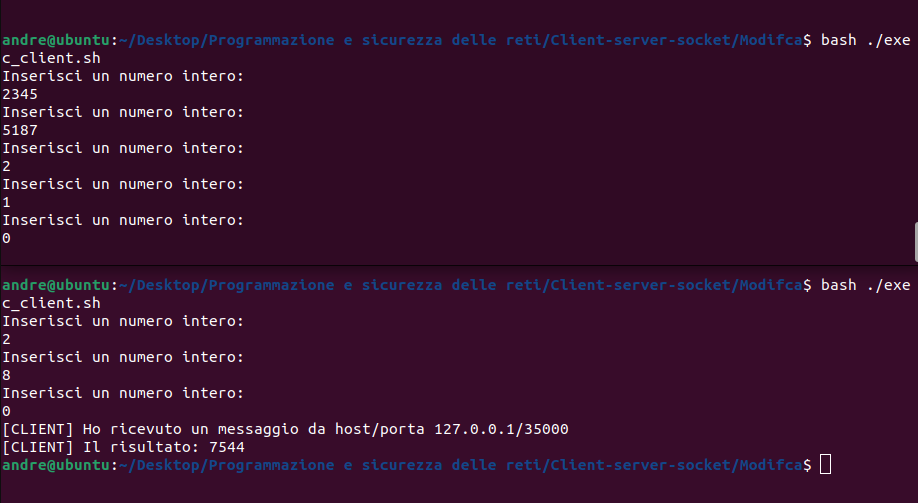
\includegraphics[width=\textwidth]{img/soluzioni_TCP-UDP/TCP-UDP_5.png}
	\end{figure}
	
	\noindent
	Ricordando di eseguire prima un'operazione del client A, poi un'operazione del client B, poi A, poi B, e così via. Il risultato ottenuto sul server è il seguente:\newpage
	\begin{figure}[!htp]
		\centering
		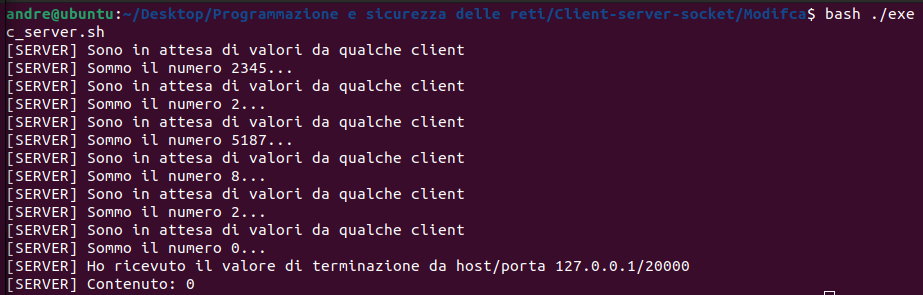
\includegraphics[width=\textwidth]{img/soluzioni_TCP-UDP/TCP-UDP_6.png}
	\end{figure}

	\noindent
	Quindi, nel client B viene letta la somma corretta, ovvero quella eseguita prima che il client B inviasse il valore zero e richiedesse la terminazione del server. Al contrario, nel client A il valore inserito 1 non viene ricevuto dal server, ma dato che è un protocollo UDP, il client continua ad eseguire il codice. Il problema nel client A sorge nel momento in cui esce dal ciclo \textsf{do...while}, poiché deve attendere una risposta (il risultato) dal server. Tuttavia, dato che il client B ha inviato il valore di terminazione \dquotes{0} e di conseguenza ha cessato la sua esecuzione, il client A rimarrà in un stato di attesa infinito.\newline
	
	\noindent
	Quale potrebbe essere una \textbf{possibile modifica per evitare questa attesa infinita}? Ci sono molteplici soluzioni, una tra queste è quella di inserire un ciclo \textsf{do...while} al termine del codice del server e inserendo al suo interno un'attesa di ricezione con il conseguente invio del valore corretto. Il codice muterebbe in questo modo:
	\lstinputlisting[language=C]{code/serverUDP_inc_mod3.c}
	E l'esecuzione del client diventerebbe:
	\begin{figure}[!htp]
		\centering
		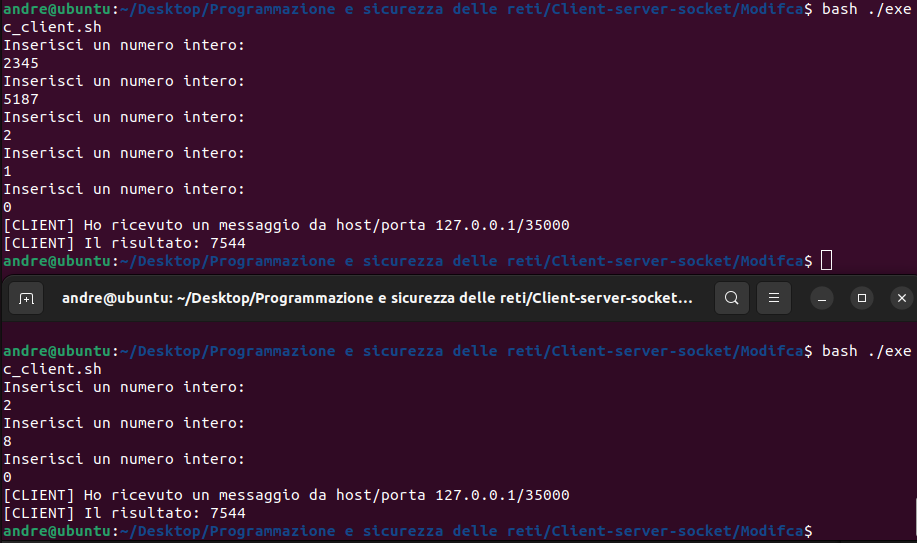
\includegraphics[width=\textwidth]{img/soluzioni_TCP-UDP/TCP-UDP_7.png}
	\end{figure}

	\noindent
	Con il server che rimarrebbe in attesa di essere terminato dal programmatore:
	\begin{figure}[!htp]
		\centering
		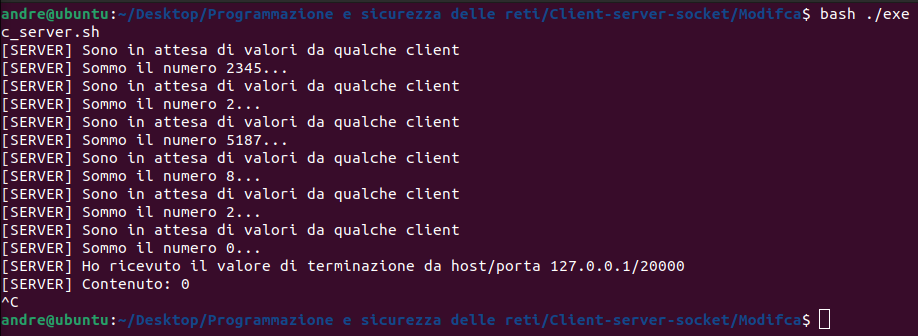
\includegraphics[width=\textwidth]{img/soluzioni_TCP-UDP/TCP-UDP_8.png}
	\end{figure}\newpage

	\subsubsection{Esercizio 11 - Sommatrice TCP}
	
	Scrivere la sommatrice (quella dell'esercizio 8 al paragrafo~\ref{esercizio 8 - Sommatrice UDP}) usando TCP, compilare ed eseguire.\newline
	
	\noindent
	\textcolor{Green4}{\textbf{\emph{\underline{Soluzione}}}}\newline
	
	\noindent
	Il codice del client:
	\lstinputlisting[language=C]{code/clientTCP.c}
	Un esempio di esecuzione del client:
	\begin{figure}[!htp]
		\centering
		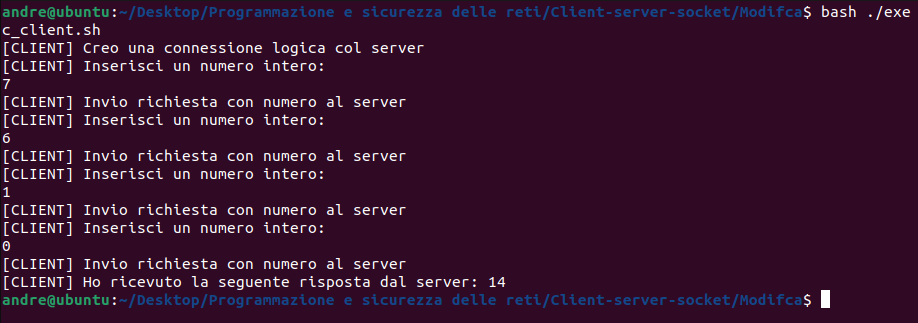
\includegraphics[width=\textwidth]{img/soluzioni_TCP-UDP/TCP-UDP_9.png}
	\end{figure}\newpage

	\noindent
	Il codice del server:
	\lstinputlisting[language=C]{code/serverTCP.c}
	Un esempio di esecuzione del server:
	\begin{figure}[!htp]
		\centering
		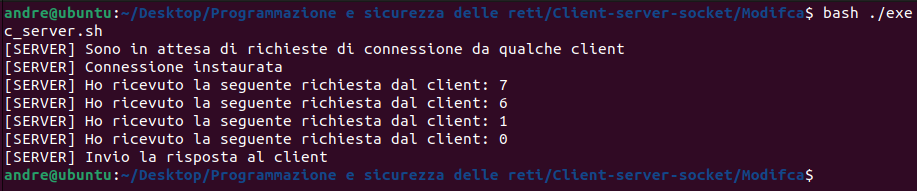
\includegraphics[width=\textwidth]{img/soluzioni_TCP-UDP/TCP-UDP_10.png}
	\end{figure}\newpage

	\subsubsection{Esercizio 12 - Sommatrice TCP e influenze reciproche}
	
	Provare a rifare l'esercizio 10 (paragrafo~\ref{esercizio 10 - Sommatrice UDP e influenze reciproche}) ma con questa nuova versione della sommatrice.\newline
	Cosa si può osservare? Che soluzioni si può trovare? C'è influenza reciproca tra i due client?\newline
	
	\noindent
	\textcolor{Green4}{\textbf{\emph{\underline{Soluzione}}}}\newline
	
	\noindent
	In questo caso, non vi è influenza reciproca poiché il protocollo TCP è più restrittivo:
	\begin{figure}[!htp]
		\centering
		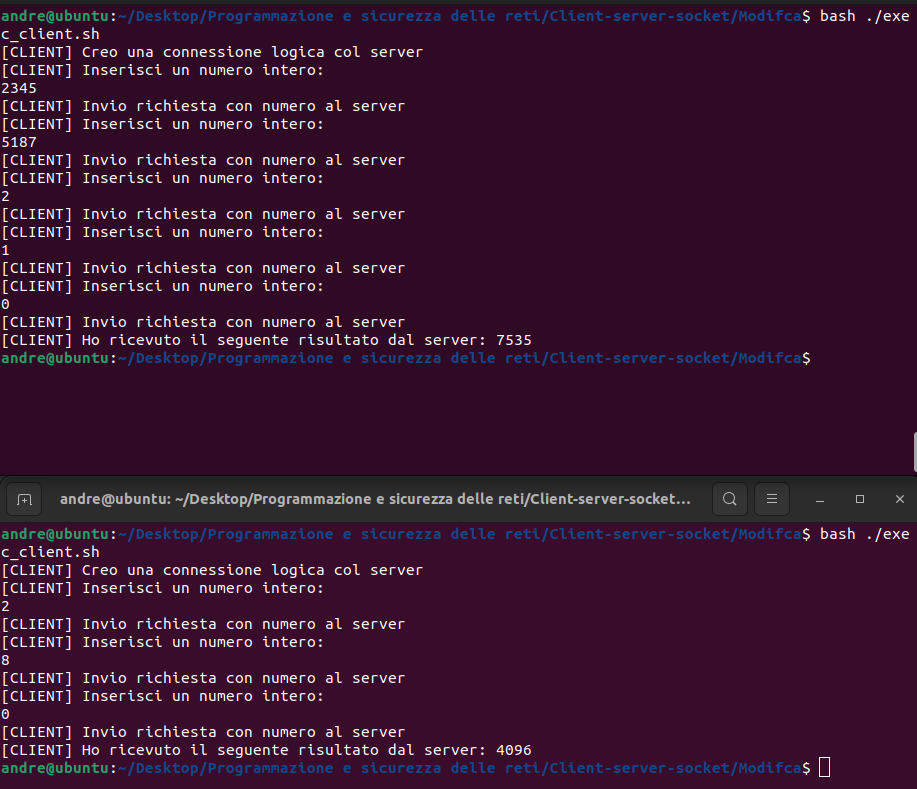
\includegraphics[width=\textwidth]{img/soluzioni_TCP-UDP/TCP-UDP_11.png}
	\end{figure}
	
	\noindent
	Il server ha la seguente esecuzione:
	\begin{figure}[!htp]
		\centering
		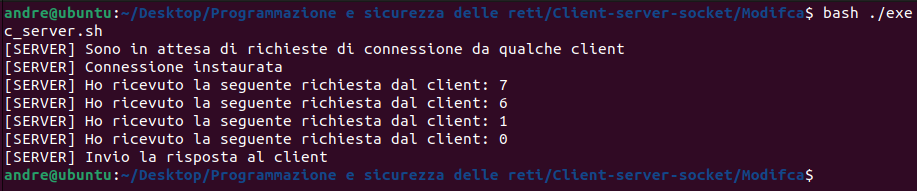
\includegraphics[width=\textwidth]{img/soluzioni_TCP-UDP/TCP-UDP_10.png}
	\end{figure}\newpage

	\subsubsection{Esercizio 13 - Sommatrice TCP e perdita di pacchetti}
	
	Riprovare l'esercizio 9 (paragrafo~\ref{esercizio 9 - Sommatrice UDP e perdita di pacchetti}) utilizzando questa volta la sommatrice TCP. Si analizzi il risultato.\newline
	
	\noindent
	\textcolor{Green4}{\textbf{\emph{\underline{Soluzione}}}}\newline
	
	\noindent
	Nonostante non sia possibile provare questo esercizio in Delta, è possibile formulare la risposta grazie alle conoscenze teoriche sul protocollo TCP.\newline
	
	\noindent
	Nel momento in cui vengono inviati i primi due valori (2345 e 5187), il server riceve correttamente il valore. Successivamente, avviene un down di rete, ovvero viene staccato il cavo. Il client tenta di inviare un pacchetto contenente il valore 2 ma fallisce. Per definizione del protocollo, entra in gioco l'RTO (\emph{Retransmission TimeOut}) che inizia ad aumentare e a riprovare l'invio finché non riesce. Alla fine del down di rete, il server riceve il pacchetto con il valore 2, successivamente riceve il pacchetto inviato dal client con il valore 1 e termina con zero.\newpage

	\subsubsection{Esercizio 14 - Trasferimento di un file}
	
	\begin{itemize}
		\item Il client chiede al server un file specificandone il nome
		\item Il server lo trasmette un byte alla volta
		\item Il client salva in locale con lo stesso nome
	\end{itemize}
	Quale protocollo si utilizza? Lanciare client e server su due macchine dierse, trasferire un file di grosse dimensioni in modo da avere il tempo di staccare e riattaccare il cavo di rete. Cosa succede al file trasferito?\newline
	
	\noindent
	\textcolor{Green4}{\underline{\textbf{\emph{Soluzione}}}}\newline
	
	\noindent
	Il protocollo utilizzato nella soluzione è il TCP. In questo modo, nel caso di eventuali perdite (ultima domanda), i due host saranno in grado di riprendere la comunicazione. Il codice del client è:
	\lstinputlisting[language=C]{code/client-Send_File.c}\newpage
	
	\noindent
	Il codice del server è:
	\lstinputlisting[language=C]{code/server-Send_File.c}






	
	\newpage

	\section{Dal Web ai Webservices}
	
	\subsection{Protocollo HTTP/HTTPS}
	
	Il \textcolor{Red3}{\textbf{protocollo HTTP}} venne inventato per fruire dei contenuti in rete (\emph{World Wide Web}). Tuttavia, al giorno d'oggi viene usato per l'invocazione di funzionalità remote, tecnica chiamata \textbf{Webservice}.\newline
	
	\noindent
	Il protocollo si divide in più \textbf{fasi}:
	\begin{enumerate}
		\item Apertura di una connessione TCP;
		
		\item Nel caso del protocollo HTTPS, avviene l'autenticazione del server e negoziazione di una chiave di cifratura;
		
		\item Invio di messaggi di \emph{request} e \emph{response};
		
		\item Chiusura della connessione TCP.
	\end{enumerate}
	\begin{figure}[!htp]
		\centering
		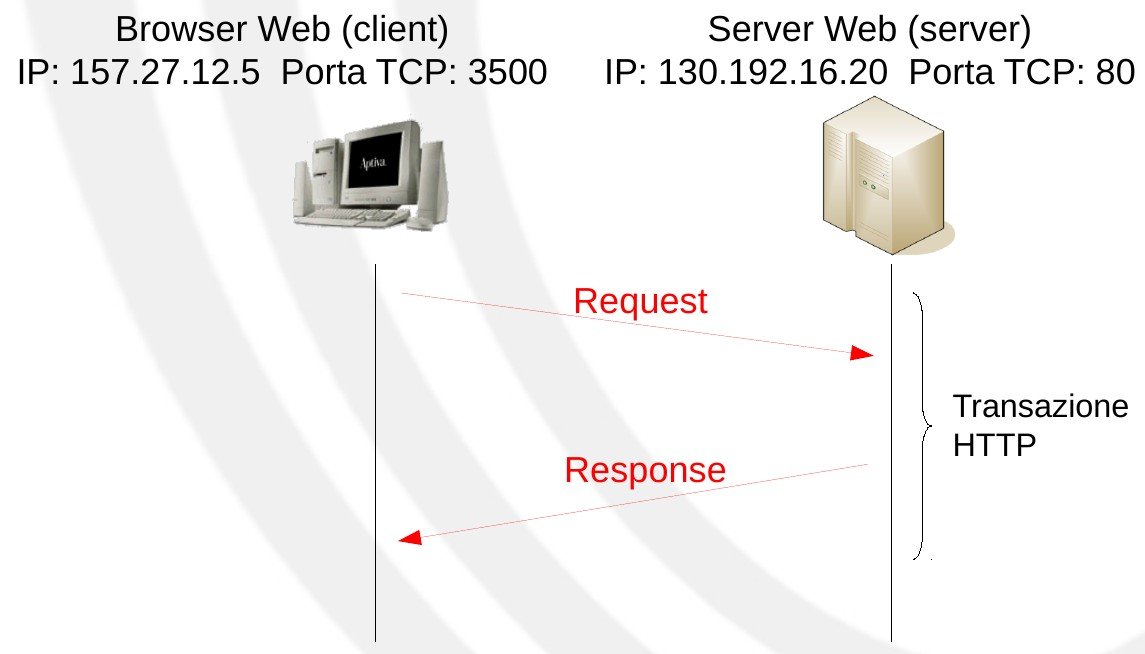
\includegraphics[width=\textwidth]{img/protocollo_http-https.png}
		\caption{Esempio di scambio di messaggi nel protocollo HTTP.}
	\end{figure}\newpage
	
	\noindent
	Nel \textcolor{Red3}{\textbf{protocollo HTTPS}} i messaggi che passano nella connessione TCP, sono gli stessi del protocollo HTTP con l'aggiunta di una \textbf{cifratura dei dati in transito} e di una \textbf{autenticazione del server mediante certificato digitale}. Inoltre, il server lavora sulla porta 443 e non sulla porta classica 80.
	\begin{figure}[!htp]
		\centering
		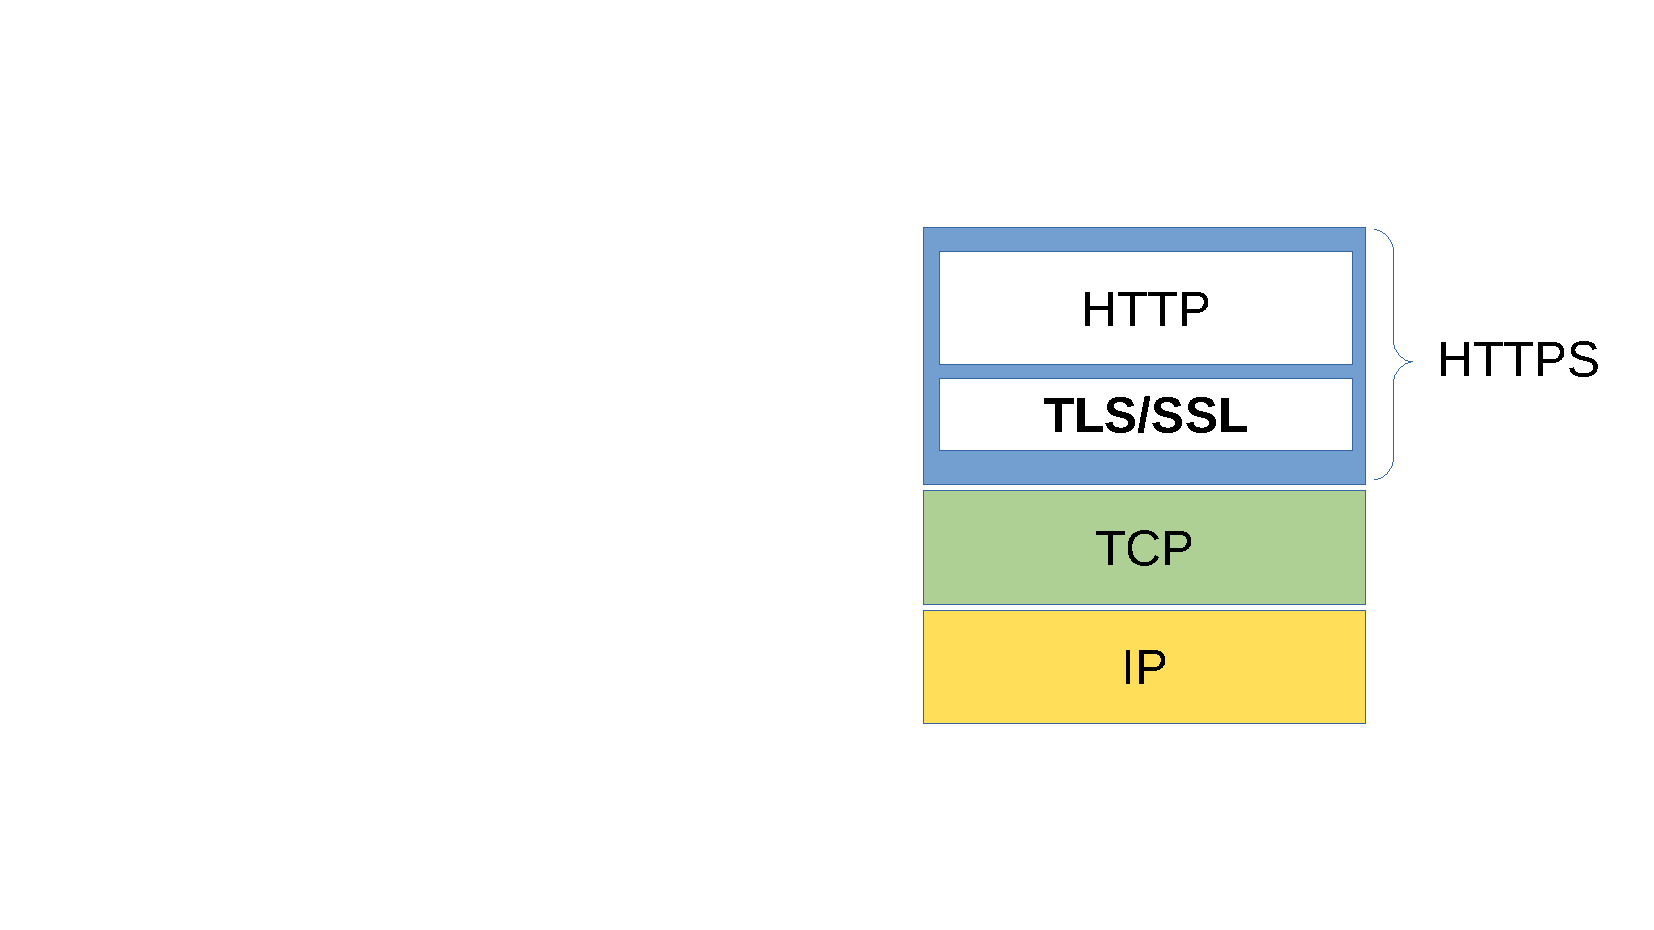
\includegraphics[width=.4\textwidth]{img/protocollo_https.pdf}
		\caption{Protocollo HTTPS.}
	\end{figure}

	\noindent
	Un \textcolor{Green4}{\textbf{esempio}} di richiesta:
	\begin{figure}[!htp]
		\centering
		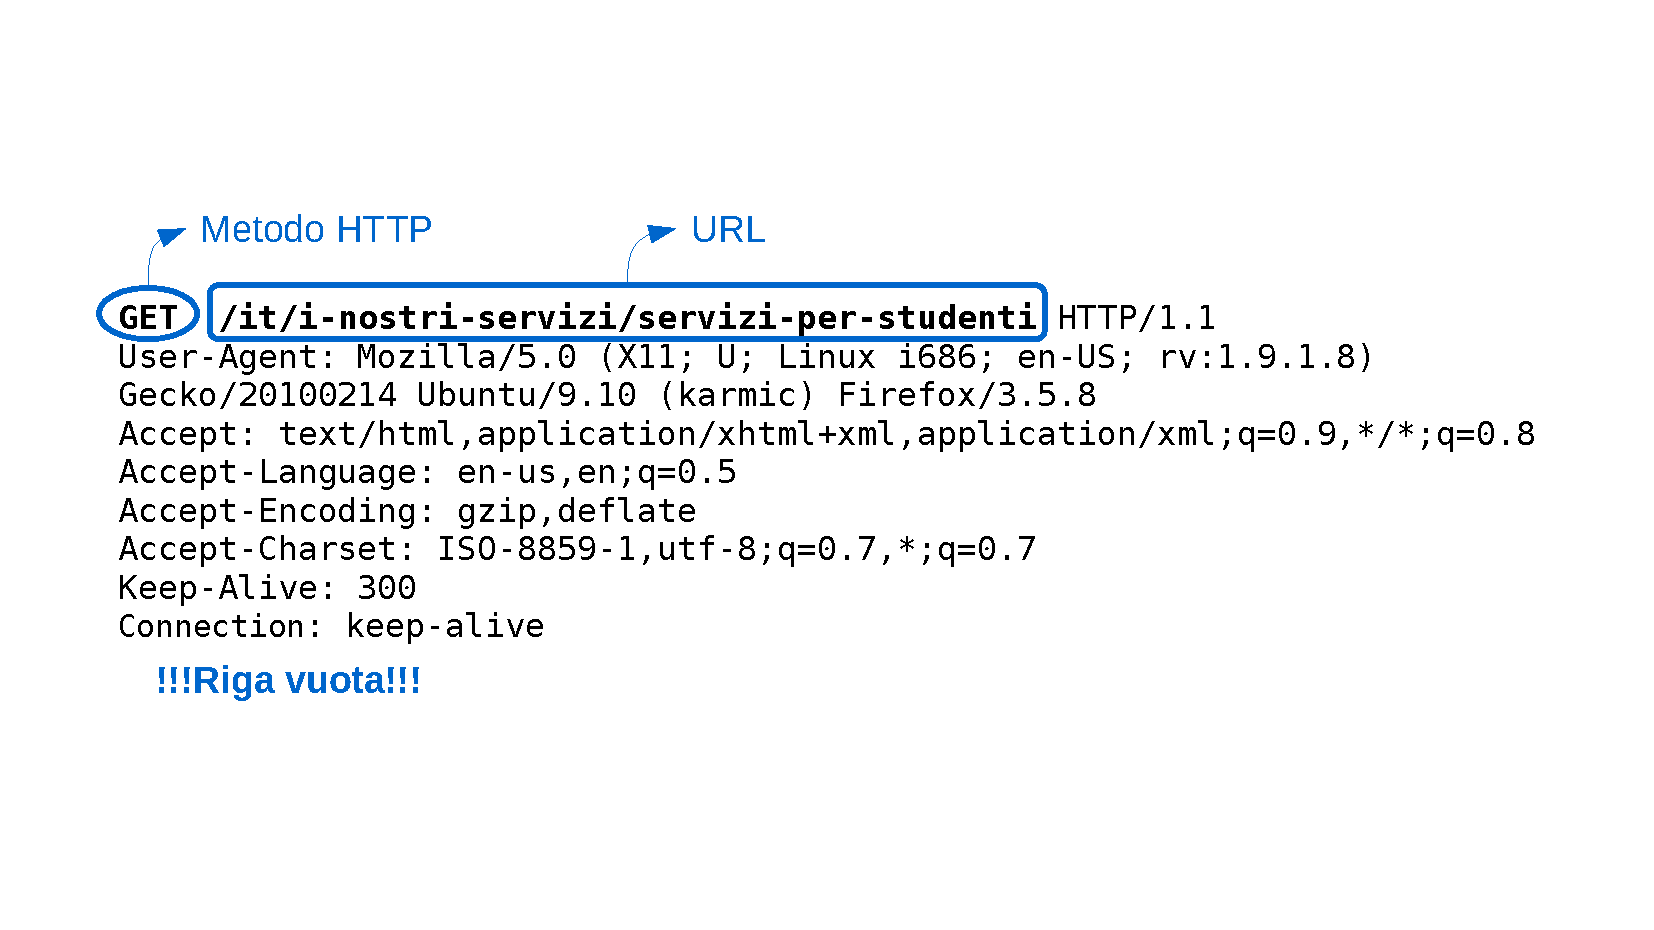
\includegraphics[width=\textwidth]{img/richiesta_http.pdf}
		\caption{Messaggio di richiesta.}
	\end{figure}

	\noindent
	Un \textcolor{Green4}{\textbf{esempio}} di risposta:
	\begin{figure}[!htp]
		\centering
		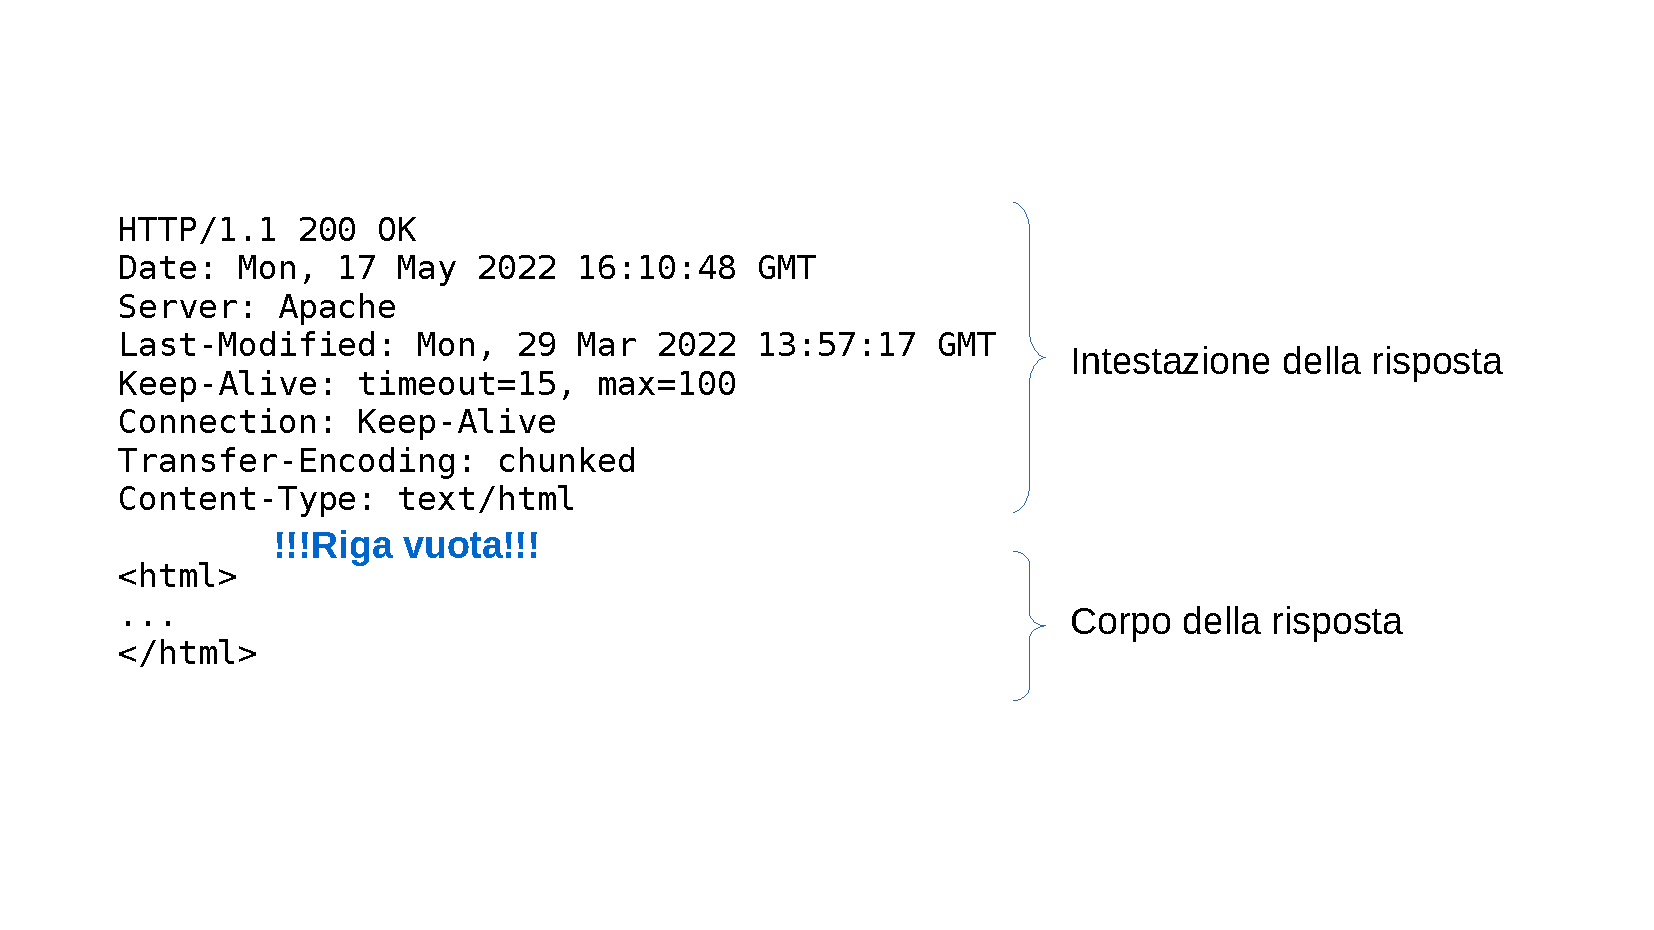
\includegraphics[width=\textwidth]{img/risposta_http.pdf}
		\caption{Messaggio di risposta.}
	\end{figure}\newpage

	\subsection{Hyper Text Markup Language (HTML) e Cascading Style Sheets (CSS)}
	
	\textcolor{Red3}{\textbf{HTML}} è un linguaggio testuale di descrizione di una pagina, in particolare è la specializzazione del generico XML (\emph{eXtensible Markup Language}). HTML si basa sui \dquotes{tag} annidati, i quali eventualmente contengono attributi.\newline
	
	\noindent
	Questo linguaggio, spesso viene utilizzato con un altro linguaggio chiamato \textbf{CSS}.\newline
	
	\noindent
	\textcolor{Green4}{\textbf{Esempi}} di codice HTML:
	\lstinputlisting[language=HTML]{code/css.html}
	E CSS:
	\lstinputlisting{code/styles.css}
	
	\longline
	
	\subsubsection{HTML: tag per richiamare immagini}
	
	Viene utilizzato \dquotes{\textsf{img src}} per richiamare le immagini:
	\lstinputlisting[language=HTML]{code/immagini.html}\newpage
	
	\subsubsection{HTML: tag per il collegamento ipertestuale}
	
	Viene utilizzato \dquotes{\textsf{href}} per il collegamento ipertestuale:
	\lstinputlisting[language=HTML]{code/link.html}
	
	\longline
	
	\subsubsection{Document Object Model (DOM)}
	
	Il \textcolor{Red3}{\textbf{Document Object Model (DOM)}} è una forma di rappresentazione dei documenti (pagina) strutturati come modello orientato agli oggetti.
	
	\longline
	
	\subsection{Javascript}
	
	\textcolor{Red3}{\textbf{Javascript}} è un linguaggio di programmazione multi paradigma orientato agli eventi, utilizzato sia nella programmazione lato client web che lato server. È facile trovarlo all'interno di codice HTML anche grazie al suo tag riconoscibile: \textsf{<script>}.
	
	Tuttavia, è difficile trovare del codice Javascript pure scritto nelle pagine HTML. Solitamente vengono create vere e proprie librerie così da rendere il codice più leggibile e mantenibile.\newline
	
	\noindent
	Un \textcolor{Green4}{\textbf{esempio}} di codice Javascript:
	\lstinputlisting[language=HTML]{code/javascript.html}\newpage
	
	\noindent
	Javascript trova il suo grande utilizzo con gli \textbf{eventi causati dall'utente}, per esempio con la pressione di un bottone all'interno di una pagina web:
	\lstinputlisting[language=HTML]{code/javascript-evento.html}
	
	\longline
	
	\subsubsection{Javascript e Document Object Model (DOM)}
	
	Il \textbf{\emph{Document Object Model} consente di trasformare una pagina web da documento statico a \emph{Graphical User Interface} (GUI)}, cioè interattivo.
	
	Infatti, grazie al codice Javascript contenuto nella pagina HTML ed eseguito dal browser, l'utente può modificare lo stato della pagina web a seconda di determinate azioni. Quindi, la pagina web si automodifica e assume le sembianze di una applicazione web, chiamata in gergo \emph{web application}.\newline
	
	\noindent
	Alcuni \textcolor{Green4}{\textbf{esempi}} di codice interattivo:
	\begin{itemize}
		\item Per avere un riquadro con la pagina web ANSA:
		\lstinputlisting[language=HTML]{code/javascript-load.html}\newpage
		
		\item Per avere un timer che alla fine del tempo stampa \dquotes{Hello}:
		\lstinputlisting[language=HTML]{code/javascript-timer.html}
		
		\item Per avere lo stesso effetto del punto precedente ma utilizzando una \textbf{funzione}:
		\lstinputlisting[language=HTML]{code/javascript-timer2.html}
	\end{itemize}\newpage
	
	\subsection[\textcolor{Red3}{\textbf{Esercizio}} di HTML e Javascript]{Esercizio di HTML e Javascript}
	
	\textcolor{Red3}{\underline{\textbf{\emph{Esercizio}}}}\newline
	
	\noindent
	Scrivere e provare una pagina HTML che ricarica periodicamente il sito dell'ANSA.\newline
	
	\noindent
	\textcolor{Green4}{\underline{\textbf{\emph{Soluzione}}}}\newline
	
	\noindent
	Il seguente codice esegue ogni due secondi il \emph{refresh} del sito:
	\lstinputlisting[language=HTML]{code/javascript-load2.html}
	
	\longline
	
	\subsection{Uniform Resource Locator (URL)}
	
	Chiamato anche Universal Resource Locator, l'\textcolor{Red3}{\textbf{URL}} consente di identificare in maniera univoca una risorsa HTTP in qualsiasi parte della rete mondiale.\newline
	
	\noindent
	È \textbf{strutturato} in tre parti:
	\begin{itemize}
		\item Il protocollo utilizzato a livello di applicazione, di trasporto e la porta utilizzata, per esempio HTTP con protocollo TCP e porta 80;
		
		\item Nome/IP dell'host che eroga tale risorsa;
		
		\item Nome della risorsa con il percorso logico completo.
	\end{itemize}\newpage
	
	\subsection[\textcolor{Red3}{\textbf{Esercizio}} su un semplice web server]{Esercizio su un semplice web server}\label{esercizio su un semplice web server}
	
	\textcolor{Red3}{\underline{\textbf{\emph{Esercizio}}}}\newline
	
	\begin{itemize}
		\item Aprire il file \textsf{serverHTTP.c} in \textsf{Esempi-web/} e analizzarne il contenuto;
		
		\item Compilarlo come nell'esercitazione sull'interfaccia socket ed eseguirlo;
		
		\item Provare ad aprire un secondo terminale nella stessa cartella e a rilanciare lo stesso server. Funziona? Perché?
		
		\item Aprire il browser preferito e impostare la URL \dquotes{\url{http://127.0.0.1:8000/}}. Cosa si vede sul browser e sul terminale?
		
		\item Aprire il browser preferito e impostare la URL \dquotes{\url{http://localhost:8000/}}. Cosa cambia?
	\end{itemize}
	
	\noindent
	\textcolor{Green4}{\underline{\textbf{\emph{Soluzione}}}}\newline
	
	\noindent
	Aprendo il file \textsf{serverHTTP.c}, il codice è il seguente:
	\lstinputlisting[language=C]{code/serverHTTP.c}
	\begin{itemize}
		\item (4-9) Vengono dichiarate le variabili necessarie per il funzionamento del server:
		\begin{itemize}
			\item \textsf{HTMLResponse} contiene la pagina web da inviare come risposta ai richiedenti;
			
			\item \textsf{sockfd} è la variabile utilizzata per creare il socket e il server;
			
			\item \textsf{connfd} è il file ricevuto tramite la connessione;
			
			\item \textsf{i} è utilizzata all'interno dei cicli;
			
			\item \textsf{length} è la lunghezza della richiesta;
			
			\item \textsf{request} è la richiesta del client, \textsf{method} è il metodo HTTP (POST, GET, ...) e \textsf{c} è una variabile temporanea utilizzata per stampare il contenuto del file.
		\end{itemize}
		
		\item (11-15) Viene creata la socket sulla porta 8000 e in caso di errore il programma termina.
		
		\item (18) Si attende una richiesta di connessione per l'invio di un file descriptor (FD).
		
		\item (20-30) Al collegamento di un client, il server stampa l'intero header della richiesta sul terminale.
		
		\item (32-37) Se viene eseguita una richiesta POST, viene stampato il contenuto del file passato.
		
		\item (39-46) Viene inviata come risposta la pagina web, chiusa la connessione/socket e fermato il programma.
	\end{itemize}\newpage
	
	\noindent
	Una volta compilato ed eseguito sul terminale, il server rimane in attesa di una connessione da parte di un client. Il tentativo di eseguire lo stesso programma fallisce poiché non è possibile creare un'interfaccia socket sulla porta 8000 (già occupata). Collegandosi ad una delle due pagine web (l'URL è lo stesso ma cambia solo l'alias), il risultato nel terminale è il seguente:
	\begin{figure}[!htp]
		\centering
		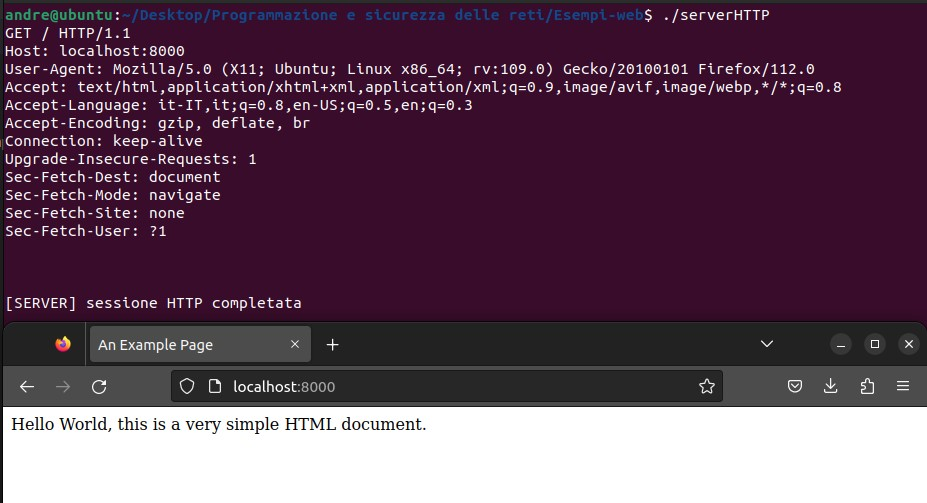
\includegraphics[width=\textwidth]{img/web-server/web-server-1.jpg}
	\end{figure}\newpage
	
	\subsection{Passare dei dati al server web col metodo GET}
	
	Il codice HTML per utilizzare il metodo GET è il seguente:
	\lstinputlisting[language=HTML]{code/form-get.html}
	La pagina web visualizzata è la seguente:
	\begin{figure}[!htp]
		\centering
		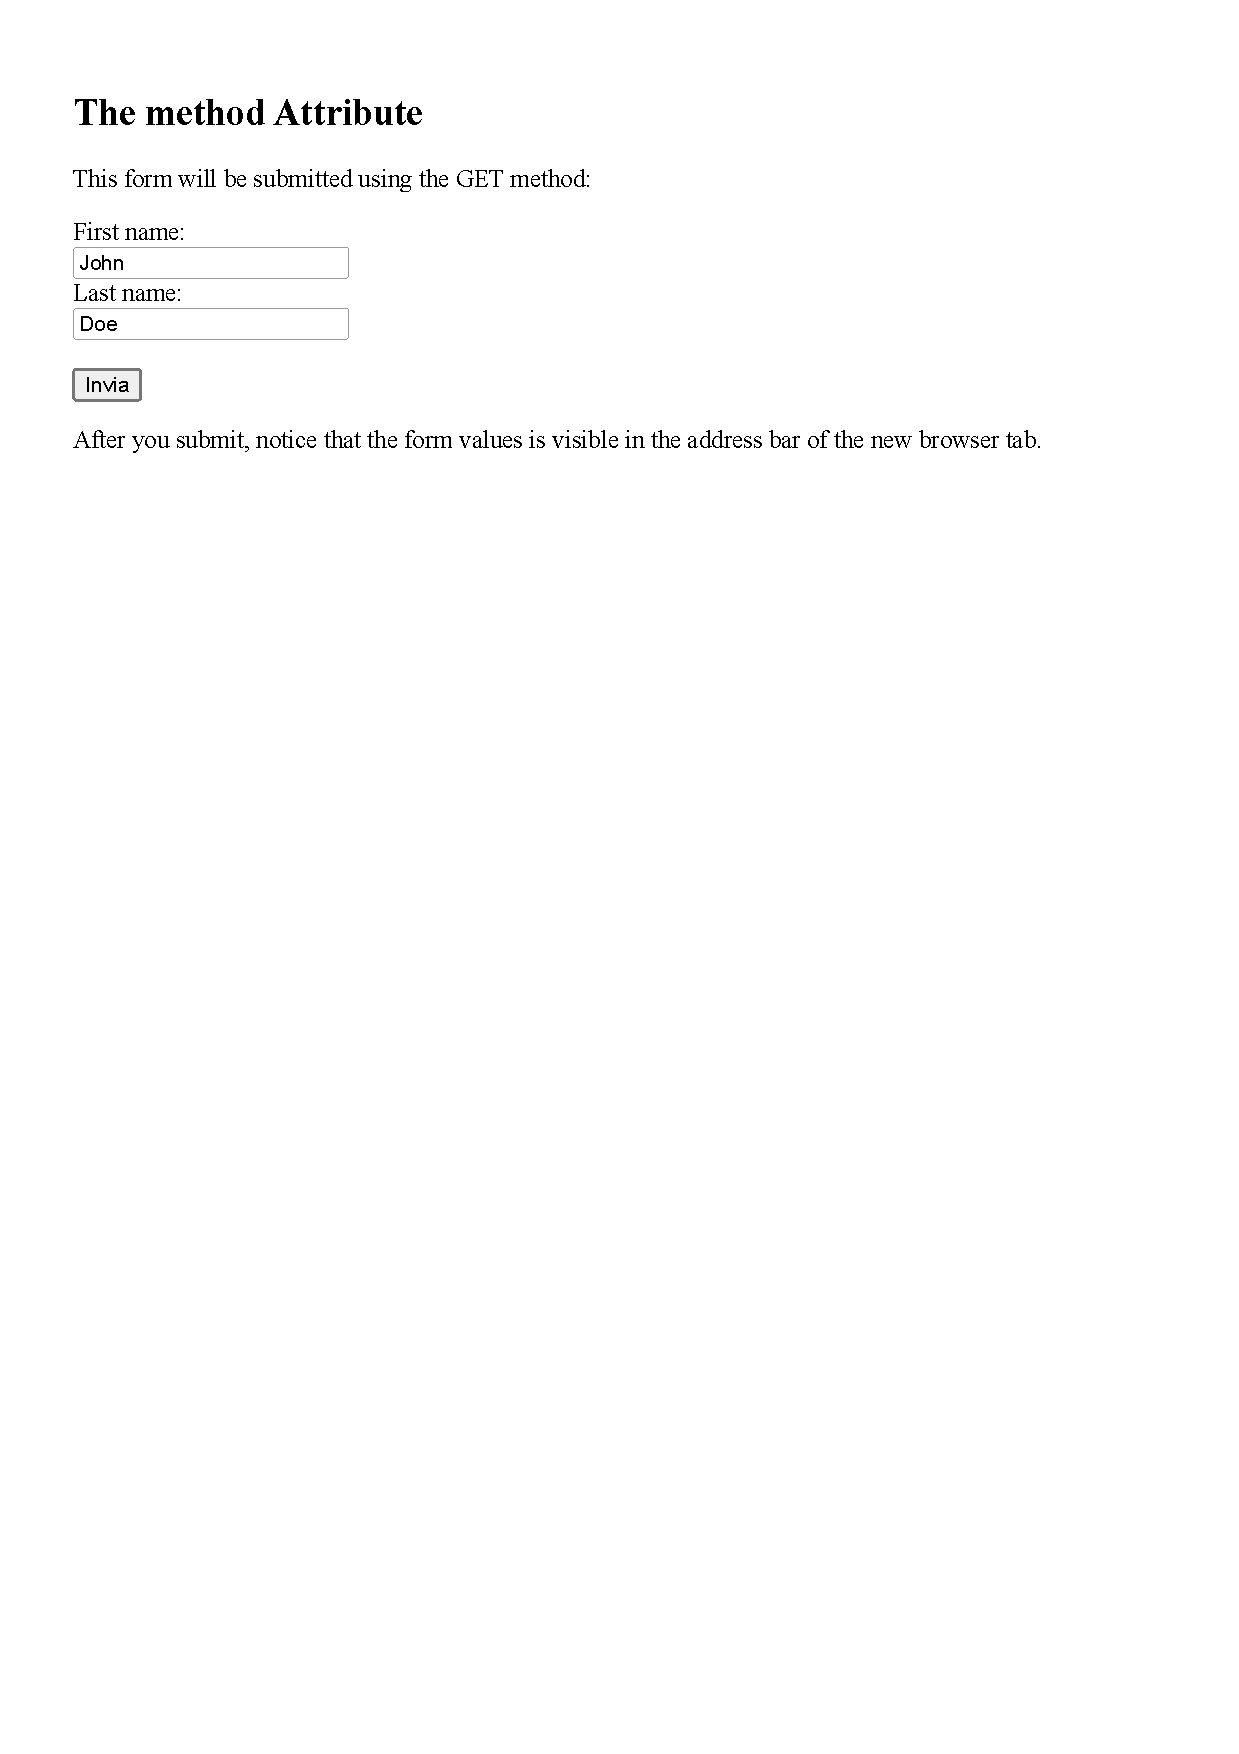
\includegraphics[width=\textwidth]{img/form-get.pdf}
	\end{figure}
	
	\noindent
	Una volta inserito nome e cognome, alla pressione del tasto, i dati saranno inviati al \emph{localhost} aggiungendo come parametri nell'URL \textsf{fname=name} e \textsf{lname=name}, dove al posto di name vengono inseriti nome e cognome. Il link risulta: \url{http://127.0.0.1/action?fname=John&lname=Doe}.\newpage
	
	\begin{figure}[!htp]
		\centering
		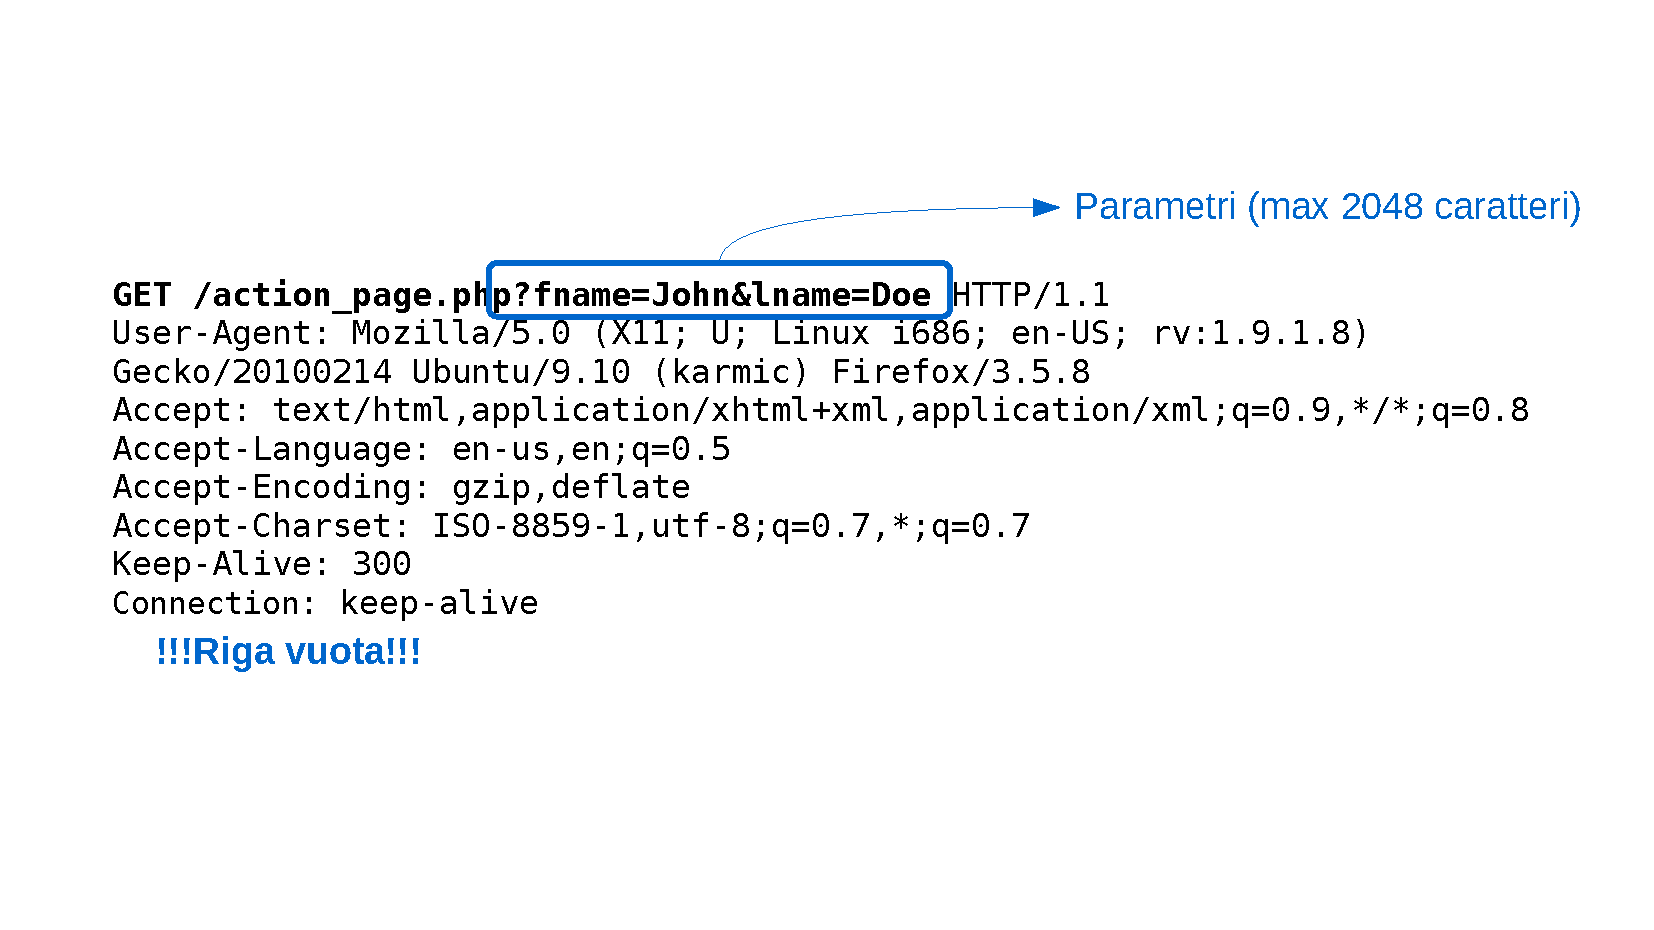
\includegraphics[width=\textwidth]{img/richiesta_get.pdf}
		\caption{La richiesta GET HTTP.}
	\end{figure}
	
	\longline
	
	\subsubsection[\textcolor{Red3}{\textbf{Esercizio}}]{Esercizio}
	
	Eseguire il server web \textsf{serverHTTP.c} e con il browser preferito aprire il file \textsf{form-get.html}. Cosa si vede? Provare ad analizzare il contenuto della connessione TCP con Wireshark. Cosa si vede?\newline
	
	\noindent
	\textcolor{Green4}{\underline{\textbf{\emph{Soluzione}}}}\newline
	
	\noindent
	Avviano il server web e aprendo la pagina web, è possibile visualizzare lo stesso form visualizzabile nella pagina precedente.\newline
	
	\noindent
	Eseguendo il metodo GET, quindi cliccando su \dquotes{Invia}, ed analizzando la comunicazione con Wireshark, è possibile osservare lo scambio di messaggi tra client e server. In particolare, tralasciando i pacchetti del protocollo TCP, è possibile vedere la richiesta GET del client diretta verso il server e la risposta di quest'ultimo con il metodo OK:
	\begin{figure}[!htp]
		\centering
		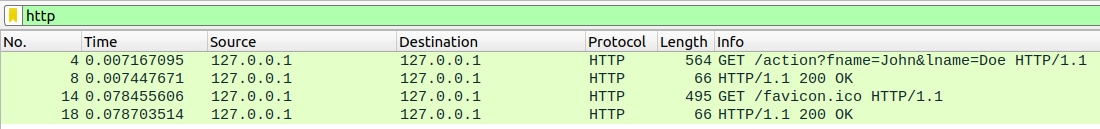
\includegraphics[width=\textwidth]{img/web-server/web-server-2.png}
	\end{figure}
	
	\noindent
	È interessante osservare anche come ogni richiesta GET venga stampata sul terminale dal server con una identazione leggibile.\newline
	
	\noindent
	Infine, è possibile notare che nell'URL della pagina web di risposta sono presenti i valori inseriti nel form. Questa è una debolezza del metodo GET che potrebbe essere sfruttata in modo malevolo.\newpage

	\subsection{Passare dei dati al server web col metodo POST}
	
	Il codice HTML per utilizzare il metodo POST è il seguente:
	\lstinputlisting[language=HTML]{code/form-post.html}
	La pagina web visualizzata è la seguente:
	\begin{figure}[!htp]
		\centering
		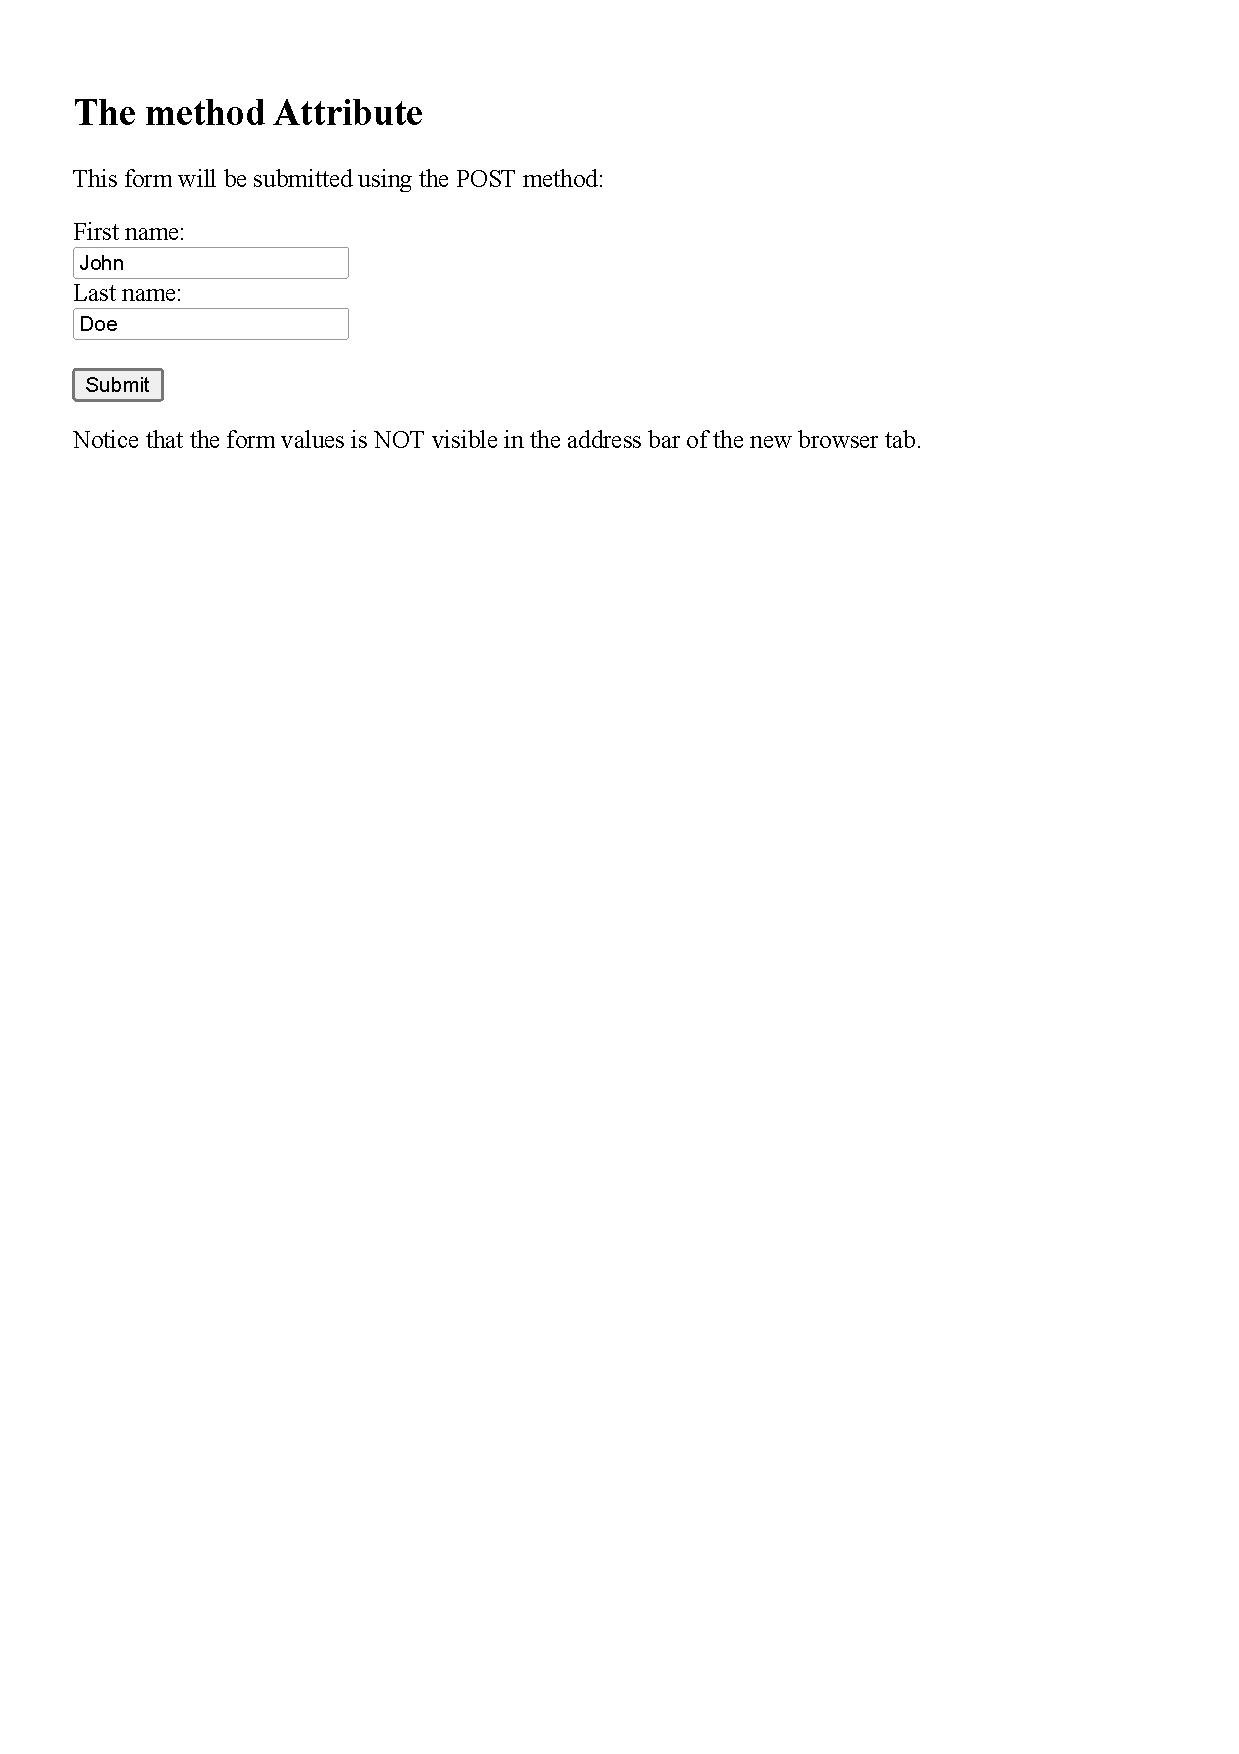
\includegraphics[width=\textwidth]{img/form-post.pdf}
	\end{figure}
	
	\noindent
	Una volta inserito nome e cognome, alla pressione del tasto, i dati saranno inviati al \emph{localhost}. \textbf{A differenza del metodo GET}, i parametri non vengono specificati nell'URL, di conseguenza la sicurezza aumenta. Il link dunque risulta: \url{http://127.0.0.1/action}.\newline
	
	\noindent
	I valori vengono inseriti all'interno della richiesta HTTP.\newpage
	
	\begin{figure}[!htp]
		\centering
		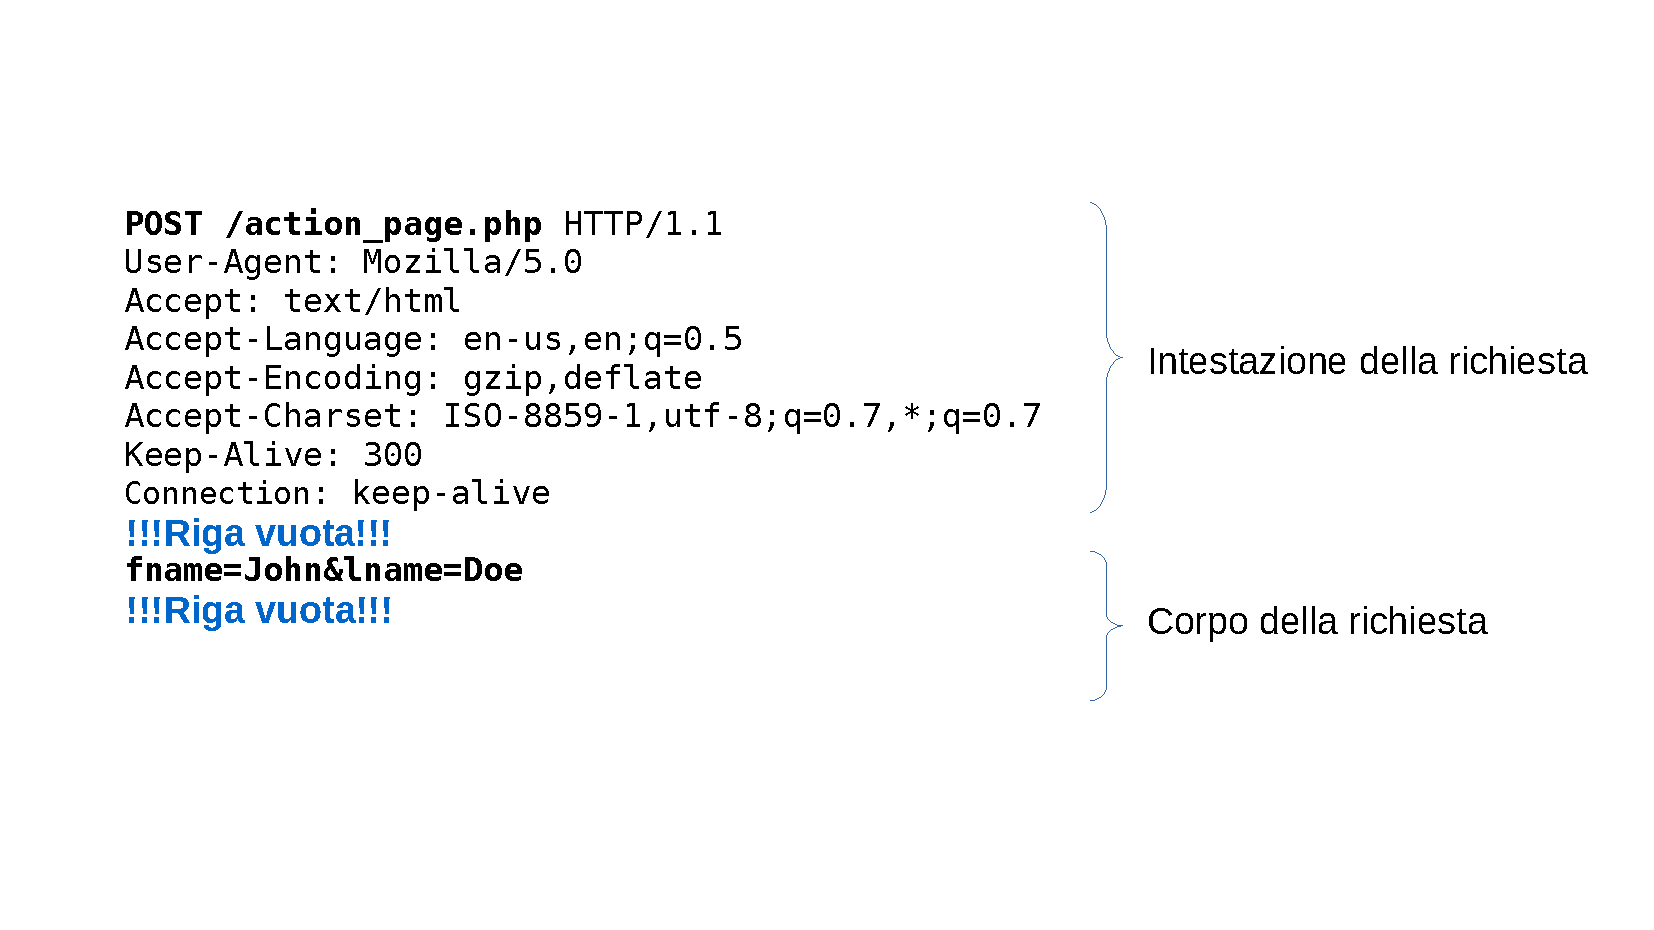
\includegraphics[width=\textwidth]{img/richiesta_post.pdf}
		\caption{La richiesta POST HTTP.}
	\end{figure}
	
	\longline
	
	\subsubsection[\textcolor{Red3}{\textbf{Esercizio}}]{Esercizio}
	
	Eseguire il server web \textsf{serverHTTP.c} e con il browser preferito aprire il file \textsf{form-post.html}. Cosa si vede? Provare ad analizzare il contenuto della connessione TCP con Wireshark. Cosa si vede?\newline
	
	\noindent
	\textcolor{Green4}{\underline{\textbf{\emph{Soluzione}}}}\newline
	
	\noindent
	Avviano il server web e aprendo la pagina web, è possibile visualizzare lo stesso form visualizzabile nella pagina precedente.\newline
	
	\noindent
	Eseguendo il metodo POST, quindi cliccando su \dquotes{Invia}, ed analizzando la comunicazione con Wireshark, è possibile osservare lo scambio di messaggi tra client e server. In particolare, tralasciando i pacchetti del protocollo TCP, è possibile vedere la richiesta POST del client diretta verso il server e la risposta di quest'ultimo con il metodo OK:
	\begin{figure}[!htp]
		\centering
		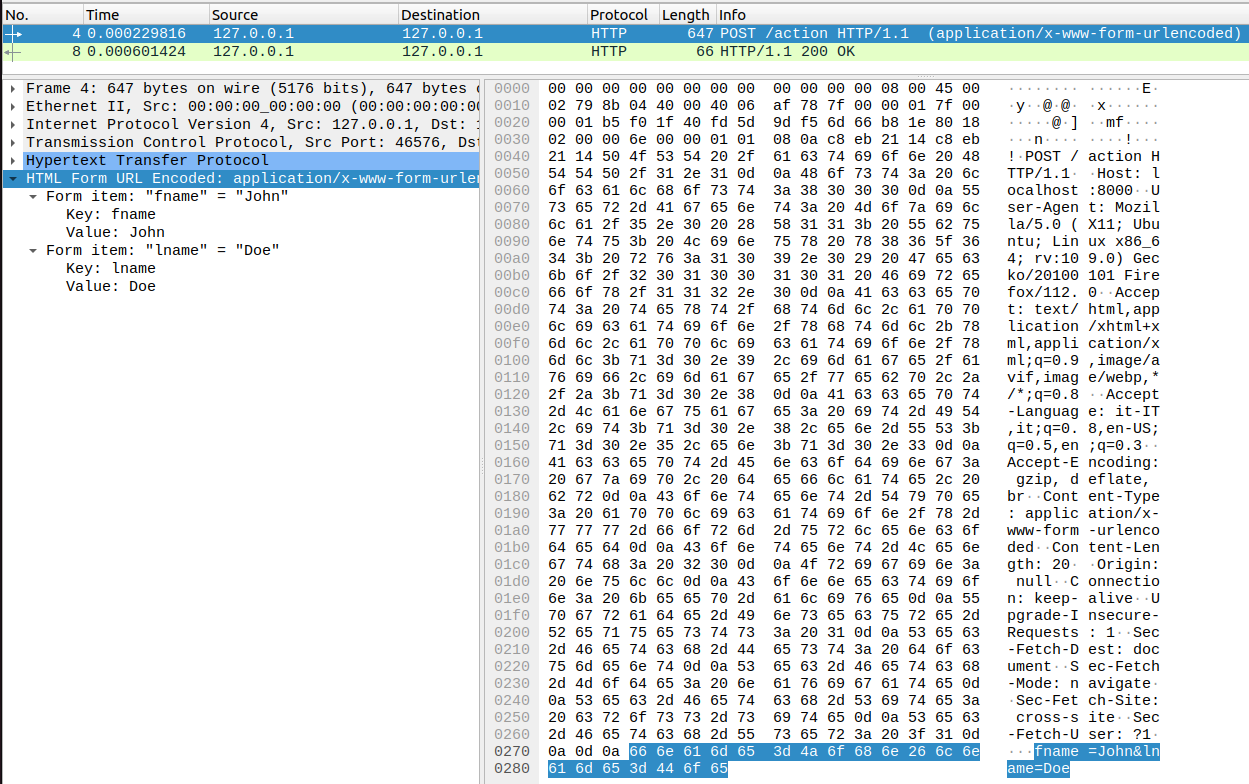
\includegraphics[width=\textwidth]{img/web-server/web-server-3.png}
	\end{figure}
	
	\noindent
	È interessante osservare anche come ogni richiesta POST venga stampata sul terminale dal server con una identazione leggibile.\newline
	
	\noindent
	A differenza del metodo GET, il metodo POST non consente di visualizzare i valori direttamente nell'URL, ma solo all'interno della richiesta. Quindi, è necessario uno \emph{sniffer} per catturare i dati.\newpage
	
	\subsection[\textcolor{Red3}{\textbf{Esercizi}} di modifica del web server]{Esercizi di modifica del web server}
	
	\subsubsection{Esercizio 1 - Ricerca di una pagina in locale}
	
	Modificare il file \textsf{serverHTTP.c} in modo che, invece di restituire sempre la solita pagina web di prova, restituisca una delle pagine html usate nel capitolo attraverso l'uso del browser. Suggerimenti:
	\begin{itemize}
		\item Provare a fare la nuova richiesta col browser usando il \textsf{serverHTTP.c} in modo da vedere la richiesta HTTP per capire dove si trova la stringa con il nome del file nella richiesta che fa il browser (aiutarsi anche con Wireshark)
		\begin{itemize}
			\item Cosa devo scrivere nella barra del browser?
		\end{itemize}
		
		\item Capire come recuperare la stringa con il nome del file della richiesta HTTP (si veda \textsf{esempio-parser.c});
		
		\item Per costruire la risposta riciclare parte del codice usato nell'esercizio del trasferimento di file.
	\end{itemize}
	Prova finale: cosa succede se chiedo al server di restituire i file \textsf{form-get.html} e \textsf{form-post.html}?\newline
	
	\noindent
	\textcolor{Green4}{\underline{\textbf{\emph{Soluzione}}}}\newline
	
	\noindent
	Il codice necessita di alcune modifiche. L'esercizio richiede l'accesso completo alla cartella in cui è presente il server. Infatti, il client deve essere in grado di richiamare la pagina all'interno della cartella, scrivendo nell'URL la pagina interessata. Per esempio, scrivendo \url{http://localhost:8000/css.html}, il server dovrebbe inviare il file \textsf{css.html} al client e quest'ultimo visualizzare la pagina web. Il codice:
	\lstinputlisting[language=C]{code/serverHTTP-ex1.c}
	\begin{itemize}
		\item (4-12) Vengono dichiarate nuove variabili ed eliminate le vecchie. Vengono dichiarate variabili per eseguire lo \emph{split}, necessario per capire quale file ha richiesto il client, per eseguire la lettura del file in locale (\textsf{buffer}) e un puntatore al file.
		
		\item (23-27) Oltre a prendere la richiesta (GET, POST, ecc), viene copiato il contenuto di \textsf{request}, il quale verrà modificato alla riga 27 a causa della funzione \textsf{strtok}\footnote{La funzione \textsf{strtok} esegue una divisione di stringhe a seconda del delimitatore impostato (\href{https://www.tutorialspoint.com/c_standard_library/c_function_strtok.htm}{link approfondimento})}.
		
		\item (44-47) Come detto in precedenza, vengono eseguite due \textsf{strtok} per acquisire il nome del file inserito dall'utente. Dato che la richiesta sarà nella forma del tipo:
		\begin{equation*}
			\textsf{GET /form-get.html HTTP/1.1}
		\end{equation*}
		Viene utilizzato un primo delimitatore \emph{slash} e \emph{spazio} (\dquotes{\textsf{/ }}) per dividere la stringa in più parti e infine viene riutilizzata la funzione \textsf{strtok} per prendere il nome del file.
		
		\item (49-56) Il server tenta di aprire il file specificato dal client. Nel caso in cui il puntatore \textsf{fptr1} rimanga nullo, il file o non esiste o non può essere aperto. Di conseguenza, il server risponde al server con un \textsf{404 Not Found} e stampa l'errore.\newpage
		
		\item (57-85) In questa parte di codice l'obbiettivo è leggere il contenuto del file richiesto dall'utente e inviarglielo come pagina web.
		\begin{itemize}
			\item (61) La funzione \textsf{fseek} cambia la posizione del puntatore all'interno di un file. In questo caso, è utile posizionarsi alla fine del file (\textsf{SEEK\_END}) per capire la grandezza del file;
			
			\item (63) Come accennato precedentemente, grazie alla funzione \textsf{ftell} è possibile ottenere la grandezza del file. O meglio, quanti caratteri ci sono all'interno così di allocare uno spazio in memoria della grandezza esatta;
			
			\item (65) Dopo aver calcolato il numero di caratteri dentro il file, il puntatore del file stream viene riposizionato all'inizio (\textsf{SEEK\_SET});
			
			\item (67-69) Allocazione del buffer della lunghezza equivalente al numero di caratteri dentro il file e controllo di eventuali errori di allocazione. Nel caso in cui l'allocazione sia stata eseguita correttamente, viene letto l'intero file e salvato ogni carattere all'interno della stringa \textsf{buffer};
			
			\item (77-84) Se durante la lettura da file non ci sono stati errori, viene inviata una risposta affermativa al client, quindi un codice 200 del protocollo HTTP; viene inviato l'intero contenuto del buffer, quindi del file; infine, vengono inviati dei caratteri di identazione (non necessari).
		\end{itemize}
	\end{itemize}\newpage
	
	\subsubsection{Esercizio 2 - Upload di un file sul server}
	
	Modificare il server web \textsf{serverHTTP.c} in modo che accetti con il metodo POST un intero file da salvare nella cartella del server (il cosiddetto \dquotes{upload sul server}). Suggerimenti:
	\begin{itemize}
		\item Utilizzare il file \textsf{form-file.html} con \textsf{serverHTTP.c} non modificato ed analizzare il contenuto della connessione TCP con Wireshark in modo da capire nella richiesta HTTP:
		\begin{itemize}
			\item Dove si trova il nome del file
			\item Dove si trova il contenuto del file
		\end{itemize}
		
		\item Nella lettura della richiesta HTTP sul server aggiungere il codice che salva il file prendendo spunto dal codice usato nell'esercizio del trasferimento di file;
		
		\item Invece la risposta HTTP può essere molto statica come nella versione originale di \textsf{serverHTTP.c}.
	\end{itemize}
	
	\noindent
	\textcolor{Green4}{\underline{\textbf{\emph{Soluzione}}}}\newline
	
	\noindent
	Prima di parlare del codice, è necessario fare una premessa. Quando viene inviato un file (immagine, testuale, audio, video, ...) tramite il protocollo HTTP, esso viene \dquotes{immagazzinato} all'interno di un MIME (Multipurpose Internet Mail Extensions). Tale protocollo racchiude il file all'interno di due limitatori, chiamati \emph{boundary}. All'interno di questi limitatori, è possibile trovare alcuni dati come il Content-Type o il filename (parametro da tenere sotto osservazione per questo esercizio). Una buona introduzione al protocollo è possibile trovarla qui: \href{https://en.wikipedia.org/wiki/MIME}{Wikipedia}.\newline
	
	\noindent
	Il codice si presenta un po' lungo e apparentemente complesso, ma viene fornita una spiegazione dettagliata a fine paragrafo:
	\lstinputlisting[language=C]{code/serverHTTP-ex2.c}
	\begin{itemize}
		\item (4-8) Alcune variabili sono le solite del web server iniziale, mentre altre, come \textsf{fptr1}, sono necessarie alla copia dei caratteri all'interno del nuovo file in locale sul server.
		
		\item (10-29) Il codice è lo stesso e la spiegazione è possibile trovarla nel codice sorgente (paragrafo~\ref{esercizio su un semplice web server}).
		
		\item (31) Se il metodo è di tipo \textsf{POST}, il codice accoglie il file, altrimenti invia la pagina di default classica (\textsf{HTMLResponse}) e chiude la connessione di file descriptor.
		
		\item (33-36) La variabile filename è necessaria per salvare il nome del file. Invece, la variabile \textsf{flag} viene utilizzata per verificare che prima del nome del file all'interno del pacchetto HTTP, ci sia la stringa \textsf{filename}. Quindi, se sia effettivamente il nome del file e non ci si trovi in un altro punto.
		
		\item (39-148) Il vero \emph{core} del codice. Il ciclo è apparentemente infinito e continua a leggere dalla pipe socket, tutti i dati inviati dal client. L'iterazione si conclude nel momento in cui è stata svuotata l'intera pipe:
		\begin{itemize}
			\item Prima di iniziare a descrivere il codice, è importante capire la struttura di un MIME. Nella seguente immagine è possibile osservare la struttura del pacchetto dopo l'upload di un file chiamato \dquotes{\textsf{upload.sh}}:
			\begin{figure}[!htp]
				\centering
				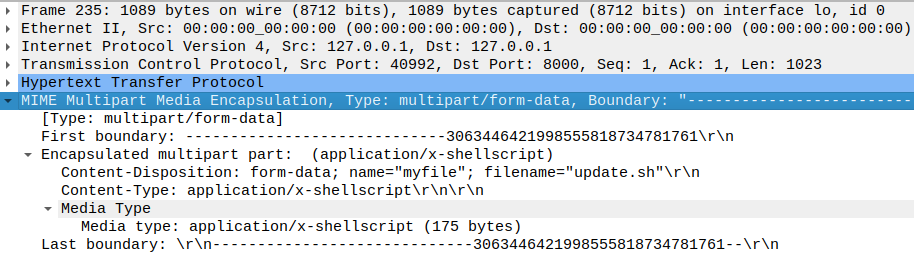
\includegraphics[width=\textwidth]{img/web-server/web-server-4.png}
				\caption{Esempio di struttura del protocollo MIME.}
				\label{esempio di struttura del protocollo MIME}
			\end{figure}
			
			\noindent
			Nell'immagine è possibile vedere i due \emph{boundary} che delimitano il contenuto. All'interno è possibile trovare il nome del file (\textsf{update.sh}), il tipo di contenuto, quindi uno script della shell (\emph{shellscript}) e ovviamente il contenuto del file in bytes.\newline
			N.B.: a fine di ogni linea ci sono alcuni \emph{escape characters}. Essi sono molto importanti.
			
			\item (41-89) Per leggere il nome del file, si esegue questo pezzo di codice:
			\begin{itemize}
				\item (41-46) Viene effettuata la lettura del contenuto. Nel caso in cui la \textsf{flag} sia a 1, quindi ancora non è stato trovato il \textsf{filename}, e il carattere letto corrisponde al punto e virgola \textsf{;}, si inizia la possibile lettura del \textsf{filename}.\newline
				Perché il carattere letto deve essere \textsf{;}? Analizzando il pacchetto MIME, è facilmente visibile che uno dei pochi parametri che non può cambiare è il \textsf{;} o il \textsf{form-data}, ecc. In questo caso, viene preso il punto e virgola come riferimento.
				
				\item (48-61) Supponendo quindi che la lettura di ogni singolo carattere sia vicino a \textsf{filename}, eseguendo due letture (49 e 53), si dovrebbe leggere uno spazio e poi la \textsf{f} (iniziale del parametro \textsf{filename}). Per verificare che la supposizione sia vera, viene controllata tale condizione (55). Se la parola inizia con la \textsf{f}, per avere una certezza in più, e anche per avanzare con la lettura del file, vengono eseguite 7 letture, quindi partendo da \textsf{f}:
				\begin{enumerate}
					\item lettura, lettera \textsf{i}
					\item lettura, lettera \textsf{l}
					\item lettura, lettera \textsf{e}
					\item lettura, lettera \textsf{n}
					\item lettura, lettera \textsf{a}
					\item lettura, lettera \textsf{m}
					\item lettura, lettera \textsf{e}
				\end{enumerate}
				
				\item (62-71) Se la sequenza è corretta, l'ultima parola letta dovrebbe essere una \textsf{e} e quindi viene verificata tale condizione (63). Il parametro \textsf{filename} all'interno del MIME è seguito poi da un uguale e un doppio apice (di solito \textsf{filename} viene scritto così dentro il MIME: \textsf{filename="nome\_file"}). Vengono effettuate due letture per scartare, e stampare, tali valori.
				
				\item (73-89) Viene creato un piccolo ciclo while che ha l'obbiettivo di leggere qualsiasi carattere che si trova all'interno del \textsf{filename}. La lettura (76) e la concatenazione nella stringa risultato (86) continuano finché non viene trovato il doppio apice (79) che chiude il valore del \textsf{filename}. Viene anche impostata la \emph{flag} a zero così da evitare eventuali controlli in futuro del filename poiché esso è già stato acquisito.
			\end{itemize}\newpage
			
			\item (91-148) Per leggere il contenuto del file che si trova all'interno dei \emph{boundary}, si esegue questo pezzo di codice:
			\begin{itemize}
				\item (91-92) Osservando la struttura del MIME a pagina~\pageref{esempio di struttura del protocollo MIME}, è possibile notare che ogni riga del protocollo termina con un \textsf{$\backslash$e} e \textsf{$\backslash$n}. Quindi, è possibile sfruttare questa caratteristica per capire quando inizia il contenuto del file.
				
				\item (94-108) In questa parte di codice vi è una serie di letture di caratteri. Viene controllata questa alternanza poiché il contenuto del file inizia dopo la sequenza: \textsf{$\backslash$r$\backslash$n$\backslash$r$\backslash$n}. Quindi, nel caso in cui vi è questa alternanza, il puntatore è all'interno del file.
				
				\item (109-116) Creazione banale in locale di un file che ha nome ed estensione quella che è stata ricevuta. L'apertura avviene in scrittura e viene controllato l'errore.
				
				\item (118-129) Inizia la lettura/scrittura vera e propria del file. Quindi, fintantoché non vi è il carattere che si trova alla fine del file, ovvero \textsf{$\backslash$r}, vengono copiati tutti i caratteri all'interno del nuovo file. Una volta copiati nel nuovo file, quest'ultimo viene chiuso.
				
				\item (131-148) Avvengono una serie di letture della pipe per consentire di svuotarla.
			\end{itemize}
		\end{itemize}
		
		\item (149-157) Il server invia una risposta di positiva di avvenuta ricezione, inviando la pagina di default. Infine, la connessione viene chiusa.
	\end{itemize}
	
	\newpage
	
	\subsection{Common Gateway Interface (CGI)}
	
	Il \textcolor{Red3}{\textbf{Common Gateway Interface (CGI)}} è una tecnologia utilizzata dai \emph{web server} per interfacciarsi con applicazioni esterne generando contenuti web dinamici.\newline
	
	\noindent
	Ogni qualvolta che un \emph{client} richiede al web server un URL corrispondente a un documento HTML, gi viene restituito un documento statico. Al contrario, se l'URL corrisponde a un programma CGI, il server lo esegue in tempo reale, generando dinamicamente informazioni per l'utente. Sostanzialmente è l'\textbf{esecuzione di un determinato programma sul server}.
	
	Di conseguenza, il browser diventa il \emph{client} di molte applicazioni di rete, per esempio la posta elettronica.
	
	\begin{figure}[!htp]
		\centering
		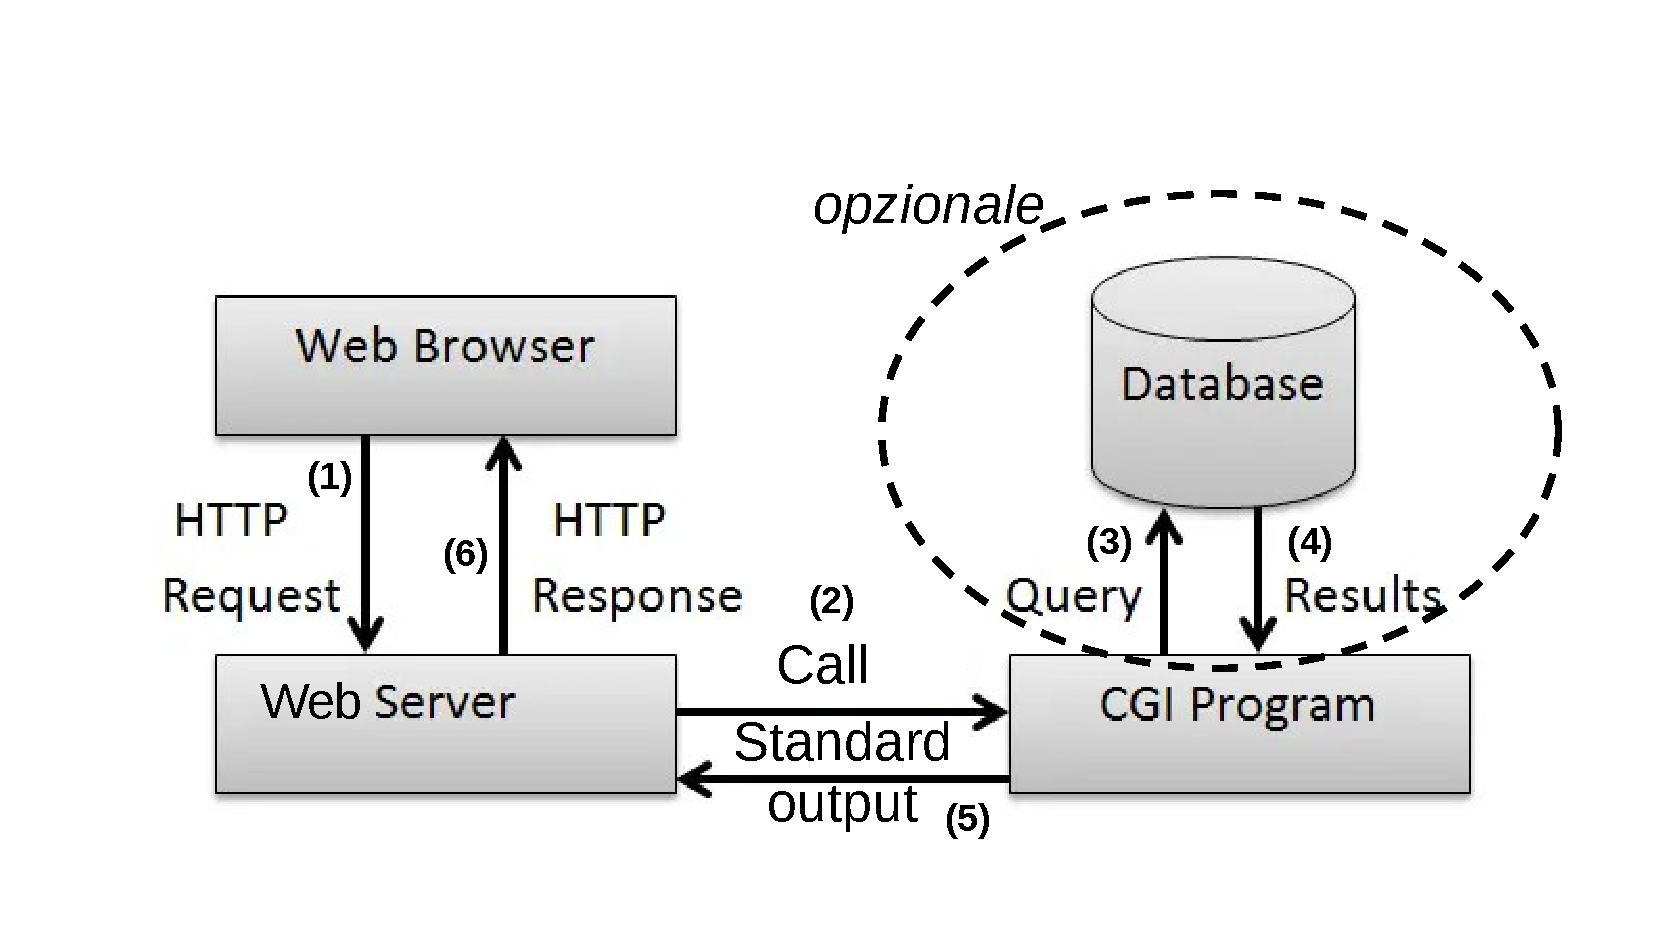
\includegraphics[width=\textwidth]{img/CGI.pdf}
		\caption{Fasi del CGI.}
	\end{figure}

	\noindent
	Degli \textcolor{Green4}{\textbf{esempi}} di esecuzione lato server di un programma sono un eseguibile come il client della posta elettronica, oppure un codice PHP, Java, NodeJS, ecc.\newpage
	
	\begin{figure}[!htp]
		\centering
		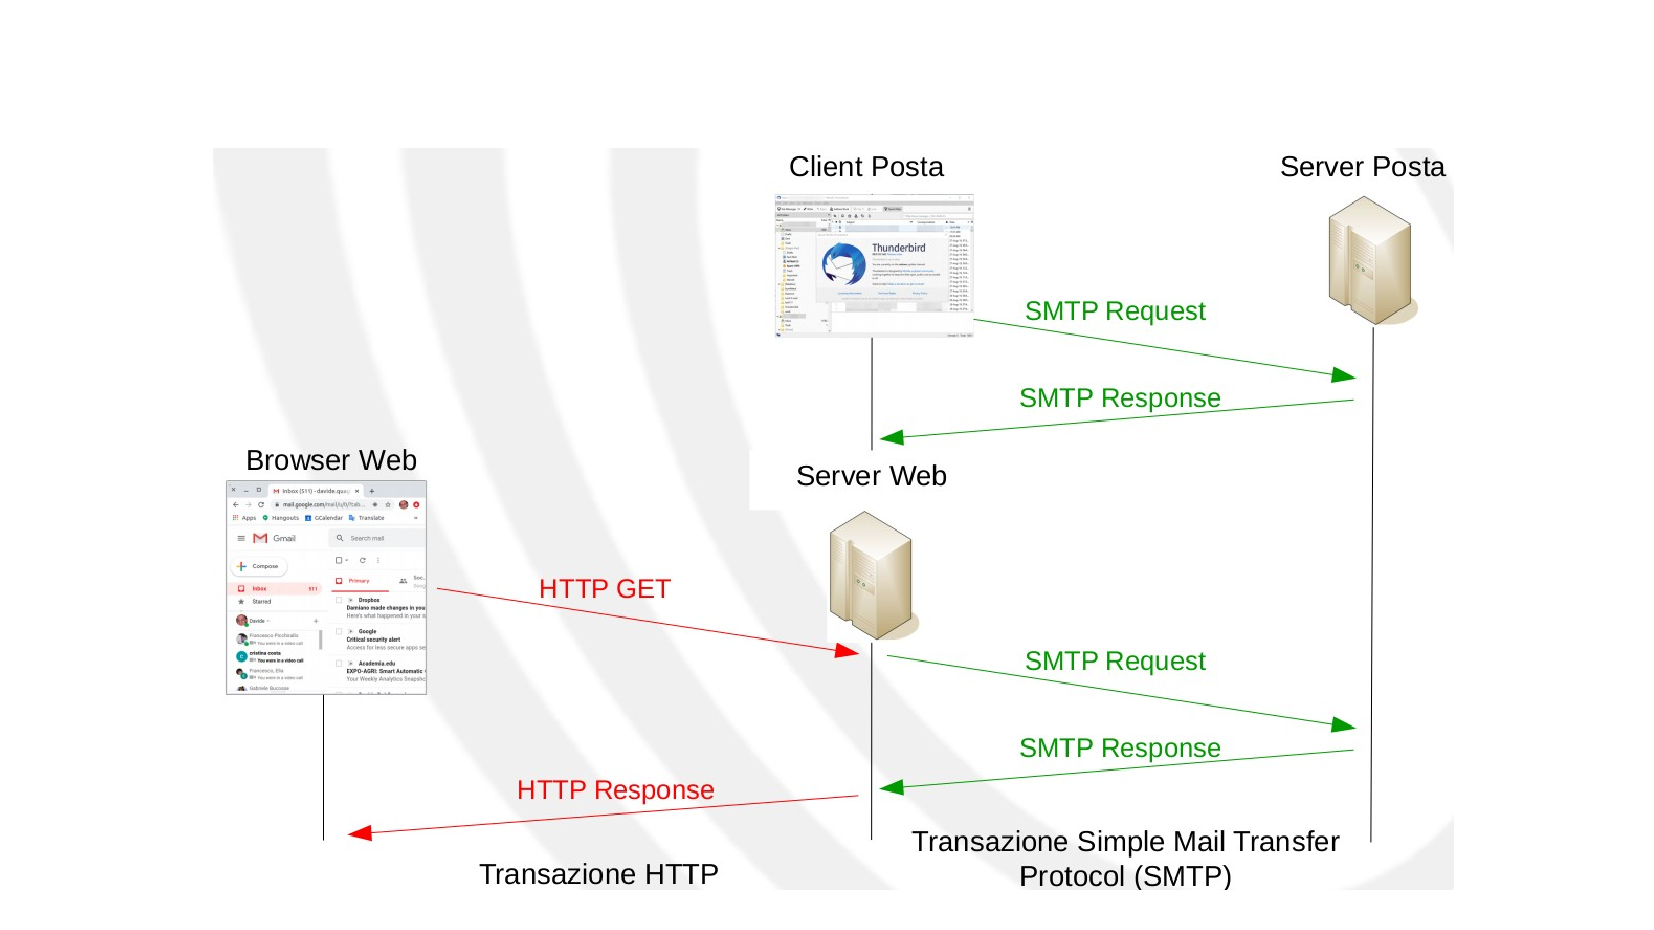
\includegraphics[width=\textwidth]{img/CGI_esempio.pdf}
		\caption{Esempio di CGI, la classica posta elettronica.}
	\end{figure}
	
	\longline
	
	\subsubsection[\textcolor{Red3}{\textbf{Esercizio}} web server esteso con gestione CGI]{Esercizio web server esteso con gestione CGI}
	
	Aprire il file \textsf{serverHTTP-CGI.c} in \textsf{Esempi-web/} e analizzarne il contenuto. Compilarlo come al solito ed eseguirlo. Aprire il browser preferito e il file \textsf{sommatrice-web.html}:
	\begin{itemize}
		\item Cosa si vede sul browser?
		\item NOTA: Provare con numeri positivi, negativi, con parte decimale...
	\end{itemize}
	A cosa corrisponde il secondo parametro della funzione \textsf{sommatrice()}?\newline
	
	\noindent
	\textcolor{Green4}{\underline{\textbf{\emph{Soluzione}}}}\newline
	
	\noindent
	Il codice del \textsf{serverHTTP-CGI.c} è il seguente:
	\lstinputlisting[language=C]{code/serverHTTP-CGI.c}\newpage
	
	\noindent
	Le uniche differenze degne di nota sono:
	\begin{itemize}
		\item (53-61) Viene controllato l'URL richiesto dall'utente. Se si tratta della pagina sommatrice, viene invocata la funzione (60) , altrimenti viene restituita la pagina statica. La funzione \textsf{strstr} consente di verificare se è presente quella sequenza di caratteri all'interno della stringa. Nel caso in cui sia presente, ritorna il puntatore al primo carattere della sequenza, altrimenti \textsf{NULL}.
		
		\item (3-18) La funzione sommatrice che prende come argomenti l'URL e la pipe di output. Le operazioni che esegue sono quelli di prendere i due operandi ed eseguire una semplice operazione di somma. La funzione si conclude con l'invio di una pagina statica contenente il risultato.
	\end{itemize}
	
	\newpage

	\subsection{Web socket}
	
	La \textcolor{Red3}{\textbf{web socket}} è una tecnologia web che fornisce canali di comunicazione chiamati \emph{full-duplex}, cioè bidirezionali, attraverso una singola connessione TCP. Viene utilizzato principalmente per realizzare applicazioni che forniscono contenuti e giochi in tempo reale. Questo perché \textbf{il protocollo consente maggiore interazione tra browser e server} grazie al alcune caratteristiche.\newline
	
	\noindent
	Innanzitutto è un \textbf{protocollo a livello di applicazione}, per cui è un \textbf{metodo alternativo a HTTP e HTTPS}. Ha la caratteristica fondamentale di \textbf{comunicazione simmetrica} tra \emph{browser} e \emph{web server}, ovverosia che \textbf{i processi possono \dquotes{prendere l'iniziativa} e inviare dei dati alla controparte}. Inoltre, nasce da una sessione HTTP/HTTPS attraverso un'operazione chiamata \textbf{Protocol Upgrade}.
	\begin{figure}[!htp]
		\centering
		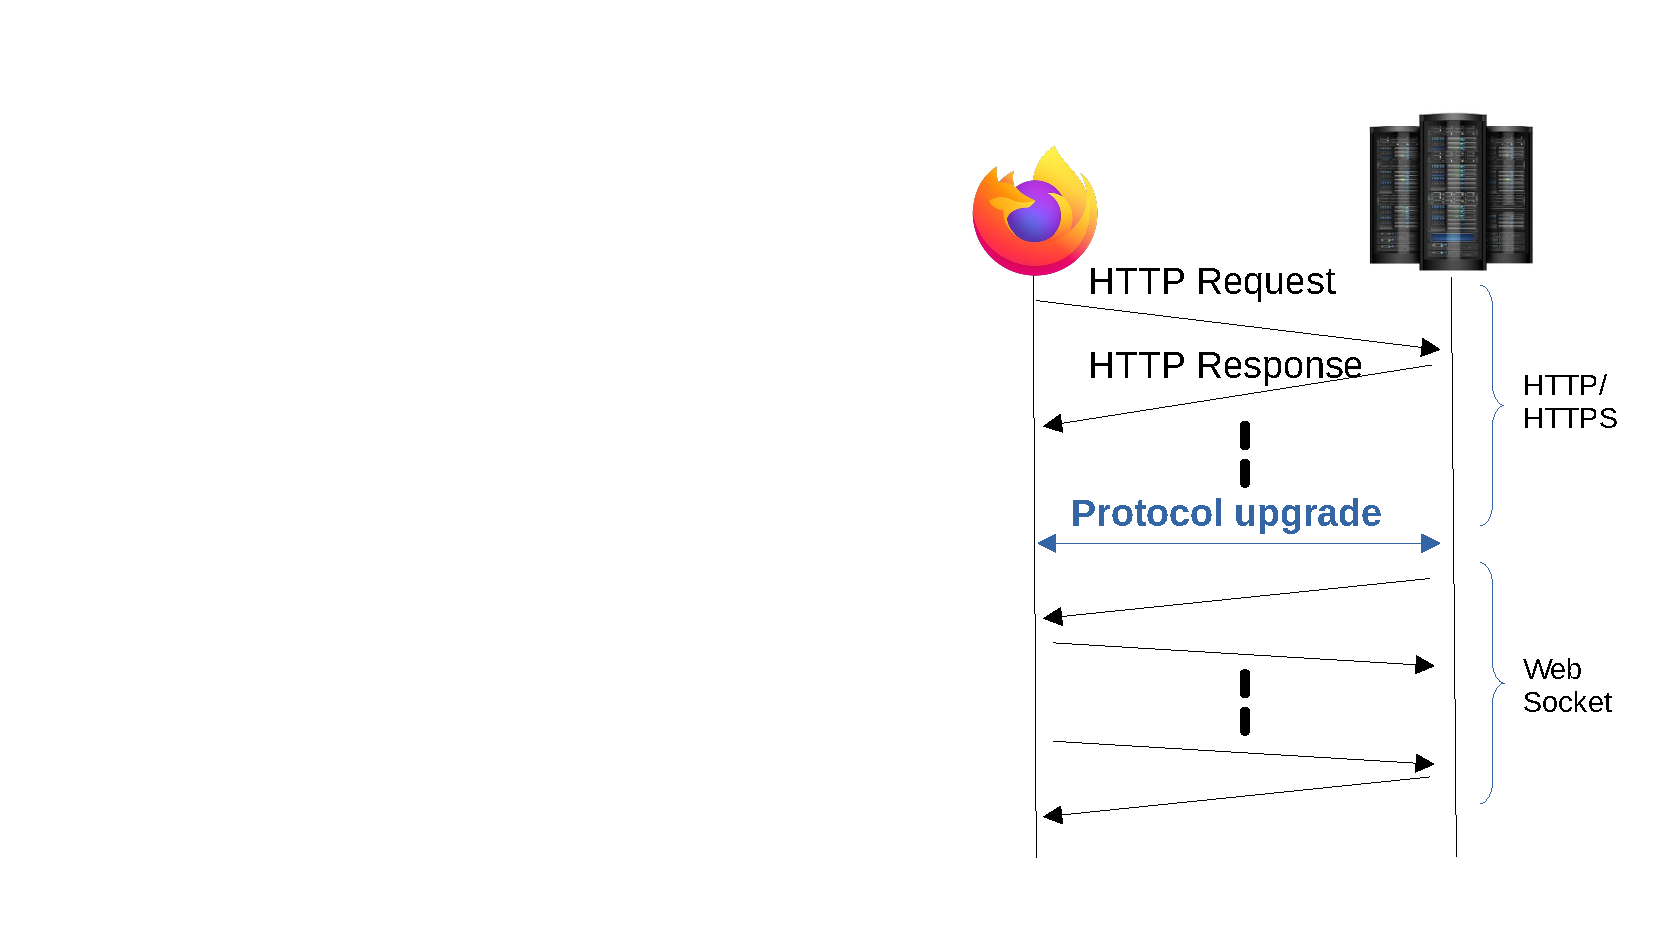
\includegraphics[width=.5\textwidth]{img/web_socket.pdf}
		\caption{Esempio di web socket e Protocol Upgrade.}
	\end{figure}
	
	\noindent
	Nel messaggio HTTP, ci sono due campi che vengono modificati per indicare il Protocol Upgrade: \textsf{Upgrade} e \textsf{Connection}. Entrambi i campi vengono modificati con i rispettivi valori \textsf{websocket} e \textsf{Upgrade}.\newpage
	
	\noindent
	\begin{figure}[!htp]
		\centering
		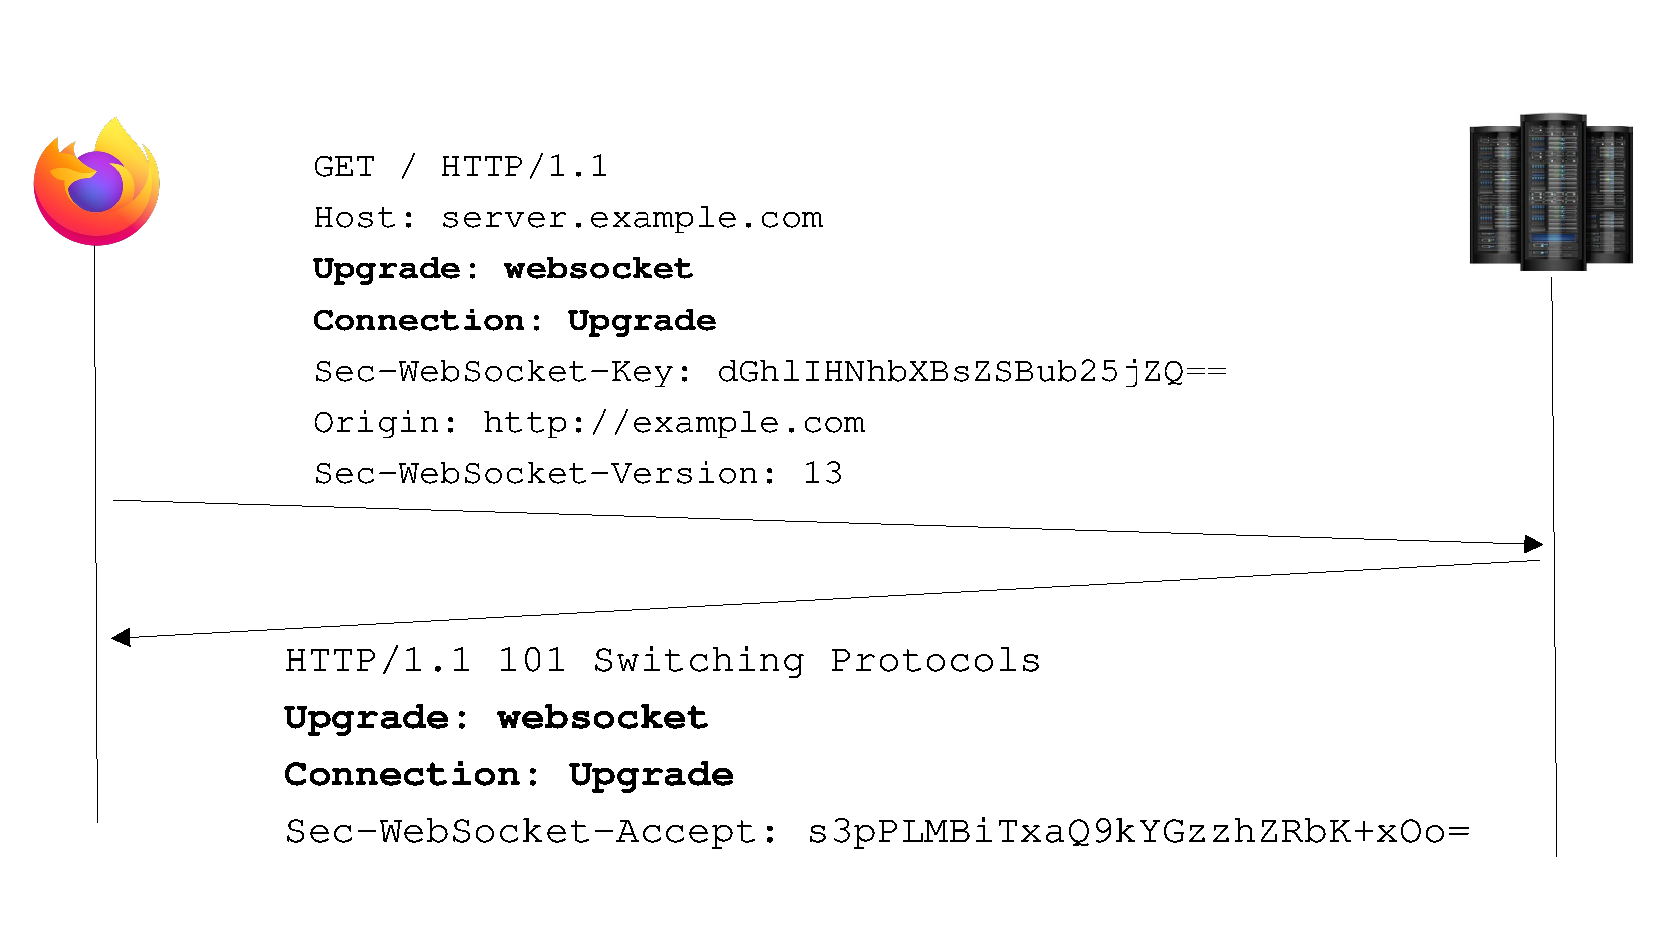
\includegraphics[width=\textwidth]{img/protocol_upgrade.pdf}
		\caption{Il Protocol Upgrade nel dettaglio.}
	\end{figure}\newpage

	\subsubsection{Approfondimento WebSocket}
	
	Il \textbf{WebSocket} è un protocollo di comunicazione web che fornisce un canale di \textbf{comunicazione bidirezionale} attraverso una singola connessione TCP inizialmente utilizzata per il protocollo HTTP.
	
	Il protocollo consente \textbf{maggiore interazione tra browser e server}, facilitando inoltre la realizzazione di applicazioni web che devono fornire contenuti in tempo reale. Tutto questo è possibile poiché i \textbf{WebSocket concedono al server di \dquotes{prendere l'iniziativa} ed effettuare dei \emph{push} autonomi di dati verso il browser per aggiornarlo}. Ovviamente questo non è possibile con il classico protocollo HTTP. Per \textbf{\emph{comunicazione bidirezionale}} si intende una comunicazione in entrambe le direzioni \underline{simultaneamente}.\newline
	
	\noindent
	I WebSocket sono basati sul protocollo TCP e nascono da una connessione HTTP grazie ad un \textbf{Upgrade Request} richiesto dal client al server. Il browser comunica questa richiesta speciale al server tramite alcune voci nell'intestazione del messaggio. Inoltre, il WebSocket consente connessioni per un lungo periodo.\newline
	
	\noindent
	In sintesi, le \textbf{\underline{caratteristiche}} di questo protocollo:
	\begin{itemize}
		\item Si \textbf{basa sul protocollo TCP}, la quale inizialmente utilizza il protocollo HTTP, ma grazie alla richiesta speciale Upgrade Request, essa muta nel protocollo WebSocket;
		
		\item \textbf{Connessione bidirezionale} (\emph{full-duplex}), quindi aumento della facilità nella realizzazione di applicazioni web che forniscono contenuti in tempo reale;
		
		\item \textbf{Utilizzo di porte note} (\emph{Well-know ports}), in particolare quelle dedicate al protocollo HTTP, quindi la 80 e la 443;
		
		\item \textbf{Connessioni per un lungo periodo}.
	\end{itemize}

	\longline
	
	\subsubsection{Limitazioni}
	
	Nonostante la grande utilità che apporta il protocollo WebSocket, esso non è la soluzione a tutto. Infatti, \textbf{HTTP ha ancora un ruolo chiave nella comunicazione client-server} per vari motivi:
	\begin{itemize}
		\item \textbf{Invio e chiusura delle connessioni per trasferimenti di dati di tipo one-time}, come i caricamenti iniziali. Il protocollo HTTP è più efficiente del WebSocket;
		
		\item \textbf{Utilizzo più intelligente} da parte di HTTP delle \textbf{risorse} grazie alla chiusura delle connessioni una volta terminate le operazioni. Al contrario, il WebSocket mantiene una connessione attiva più a lungo rischiando di sprecare risorse inutilmente;
		
		\item \textbf{WebSocket riservato solo agli utenti con JavaScript abilitato} e quindi a coloro che posseggono browser moderni a discapito, per esempio, dei sistemi \emph{embedded}.
	\end{itemize}\newpage

	\subsection{WebSocket-Chat}
	
	WebSocket-Chat è un progetto \dquotes{giocattolo} \textbf{realizzato per comprendere al meglio la tecnologia offerta dal protocollo WebSocket}. Esso utilizza vari linguaggi di programmazione: JavaScript, Node.js (\href{https://it.wikipedia.org/wiki/Node.js}{framework per realizzare applicazioni Web in JavaScript}), HTML, CSS e una parte aggiuntiva chiamata Console con Ispezione Network (monitoraggio da parte del browser con scambio tra i pacchetti).
	
	\longline
	
	\subsubsection{Node.js e l'approccio asincrono}
	
	Il framework \textcolor{Red3}{\textbf{Node.js}} (\href{https://it.wikipedia.org/wiki/Node.js}{Wikipedia}, \href{https://nodejs.org/it}{sito ufficiale Node.js}) è nato per realizzare applicazioni Web in JavaScript. Solitamente viene utilizzato lato client (\emph{client-side}) per realizzare applicazioni tipicamente lato server (\emph{server-side}).\newline
	
	\noindent
	La \textbf{caratteristica principale} di Node.js è la possibilità di accedere alle risorse del sistema operativo in modalità \emph{event-driven} (\href{https://it.wikipedia.org/wiki/Programmazione_a_eventi}{programmazione orientata agli eventi}) e \underline{non} sfruttando il classico modello basato su processi/thread concorrenti, utilizzato dai classici web server.\newline
	
	\noindent
	Il modello \textbf{\emph{event-driven}}, tradotto in programmazione orientata agli eventi, si basa sulla \textbf{mutazione di stato nel momento in cui si manifesta un evento}.
	
	A differenza della programmazione procedurale (\emph{C-style}) in cui ogni azione viene eseguita una dopo l'altra con un determinato ordine, nella programmazione ad eventi le azioni sono asincrone e seguono un ordine dettato dalla manifestazione degli eventi.\newline
	
	\noindent
	L'\textbf{approccio asincrono} comporta una \textcolor{Green4}{\textbf{grande efficienza}} soprattutto in ambito di \emph{networking} poiché capita spesso di effettuare richieste e di rimanere in attesa di un'eventuale risposta. Grazie all'approccio asincrono, \textbf{durante l'attesa possibile effettuare altre operazioni che non dipendono dalla richiesta effettuata}.
	
	\longline
	
	\subsubsection{Descrizione dell'applicazione}
	
	Il progetto mira ad avere una chat multiutente a cui collegarsi tramite browser. Le \emph{features} implementate sono le seguenti:
	\begin{itemize}
		\item Registrazione del nome di contatto che si vuole avere quando si accede alla chat.
		
		\item Invio dei messaggi in broadcast a tutti gli utenti attualmente collegati alla chat.
	
		\item Visualizzazione dei messaggi inviati col nome della persona che lo ha inviato.
	\end{itemize}\newpage

	\subsubsection{Codice Back-end server}\label{codice Back-end server}
	
	\lstinputlisting[language=JavaScript]{code/server.js}
	
	\begin{itemize}
		\item (3) \textcolor{Red3}{\textbf{Express.js}} è una libreria di Node.js che consente di costruire applicazioni web molto facilmente (\href{https://en.wikipedia.org/wiki/Express.js}{Wikipedia}, \href{https://expressjs.com/}{sito ufficiale}). L'unica cosa importante da sapere è che la prima linea di codice crea una variabile \textsf{express}, che necessita della relativa libreria Express.js, e viene \textbf{utilizzata per creare il server web in ascolto sulla porta 4000}.
		
		\item (4) \textcolor{Red3}{\textbf{Socket.IO}} è una libreria JavaScript \textbf{utilizzata per implementare il protocollo WebSocket} e racchiude molte \textbf{funzioni} tra le quali:
		\begin{itemize}
			\item \textbf{Broadcasting} a tutti i socket collegati;
			
			\item \textbf{Salvataggio} dei dati riguardanti ciascun utente;
			
			\item Approccio \textbf{asincrono di I/O}.
		\end{itemize}
	
		\item (6-13) Alla riga 7 viene effettuato il vero e proprio \emph{import} della libreria e viene creato il socket;
		
		Alla riga 11 il server si mette in ascolto, sulla porta 4000, e (riga 12) stampa sul terminale la stringa \dquotes{waiting for HTTP requests on port 4000,}.
		
		
		\item (21) Una volta ricevuta una connessione da parte di un client, il server ricerca all'interno della cartella chiamata \textsf{public}, il relativo file \dquotes{.html} da inviare al mittente.
		
		\item (29) Alla conferma di connessione instaurata e di file ricevuto, il server prende l'iniziativa ed esegue un \textbf{Upgrade Request} trasformando la connessione in una WebSocket.
		
		\item (30-38) Il server rimane in attesa, in particolare questo accade alla linea 35. Nel momento in cui un client scatena un evento, ovvero invia un messaggio con il tag \textsf{message}, il server lo inoltrerà a tutti i client connessi mediante l'oggetto \textsf{sockets}.
	\end{itemize}

	\longline
	
	\subsubsection{Codice Front-end HTML}
	
	\lstinputlisting[language=HTML]{code/index.html}
	Il codice HTML consente di far visualizzare l'interfaccia utente creata da JavaScript. In particolare, nella pagina è possibile leggere e inviare messaggi.\newline
	
	\noindent
	L'unica osservazione da fare è il tag \textsf{<script>}, il quale contiene il link del file .js da eseguire all'apertura del file HTML (paragrafo~\ref{codice Front-end JavaScript}). Ovviamente si intende il codice a riga 21, ovvero quello necessario per la chat.\newpage
	
	\subsubsection{Codice Front-end JavaScript}\label{codice Front-end JavaScript}
	
	\lstinputlisting[language=JavaScript]{code/chat.js}
	\begin{itemize}
		\item (3-6) Finché non viene inserito un nome, il codice continua a chiederlo.
		
		\item (9-13) Vengono inizializzate le variabili che acquisiscono i tag presenti nella pagina HTML.
		
		\item (15-16) Viene scritto il nome dell'utente nella pagina web e impostato il valore.
		
		\item (19) Viene creato il socket che deve connettersi al server.
		
		\item (22-30) Sul bottone di invio del messaggio, viene aggiunto un nuovo evento JavaScript. Quest'ultimo si attiverà nel momento in cui l'utente cliccherà sul bottone. Una volta premuto, se il messaggio non sarà vuoto, verrà inviato al server (con tag \textsf{message}!) il messaggio (riga 25) e il nome dell'utente (riga 26). Una volta inviato, viene svuotato il valore del messaggio.
		
		\item (32-35) Sono la stampa del messaggio ricevuto. Si noti il segno \dquotes{+=} che indica che i vari messaggi ricevuti vengono concatenati.
	\end{itemize}\newpage

	\subsubsection{Esecuzione del Front-end e del Back-end}
	
	Il server web utilizzato è Node.js che consente di eseguire codice JavaScript \emph{server-side} per creare il Back-end. Invece, il Front-end è realizzato mediante codice JavaScript eseguito dentro il browser.\newline
	
	\noindent
	Passaggi da eseguire su Windows:
	\begin{enumerate}
		\item Download del file di installazione dal sito ufficiale: \url{https://nodejs.org/it/download}
		
		\item Eseguire il Back-end:
		\begin{enumerate}
			\item Scaricare lo zip fornito su Moodle con nome \dquotes{WebSocket\_Chat};
			\item Aprire un terminale e posizionarsi nella cartella contente il file \textsf{server.js};
			\item Eseguire il comando: \textsf{node.exe server.js}.
		\end{enumerate}
		
		\item Eseguire il Front-end:
		\begin{enumerate}
			\item Aprire il browser alla pagina: \url{http://localhost:4000};
			\item (Opzionale) Aprire più finestre del browser così da simulare l'accesso da parte di più utenti.
		\end{enumerate}
	\end{enumerate}\newpage
	
	\subsubsection[\textcolor{Red3}{\textbf{Esercizi}}]{Esercizi}
	
	\noindent	
	\textcolor{Red3}{\textbf{\emph{\underline{Esercizio 1}}}}\newline
	
	\noindent
	Lanciare l'applicazione dopo aver fatto partire l'ispezione del Network tramite la console di sviluppo del browser. Ogni quanto tempo il client fa sapere al server che è ancora connesso? È un'azione dovuta all'implementazione della chat o insita nel WebSocket? A cosa sere tale procedura?\newline
	Lanciare Wireshark e vedere cosa passa in rete sulla connessione TCP interessata.\newline
	
	\noindent	
	\textcolor{Green4}{\textbf{\emph{\underline{Soluzione esercizio 1}}}}\newline
	
	\noindent
	Per analizzare la rete si utilizza il software Wireshark che consente di analizzare il flusso di pacchetti in entrata e in uscita. All'apertura del software, andando nella sezione \dquotes{\emph{Adapter for loopback traffic capture}} sarà possibile seguire tutti i pacchetti che riguardano il localhost. Per filtrare il risultato dei pacchetti, si inserisce la stringa \dquotes{websocket} nella barra in alto, così da mostrare solamente quei pacchetti con protocollo WebSocket:
	\begin{figure}[!htp]
		\centering
		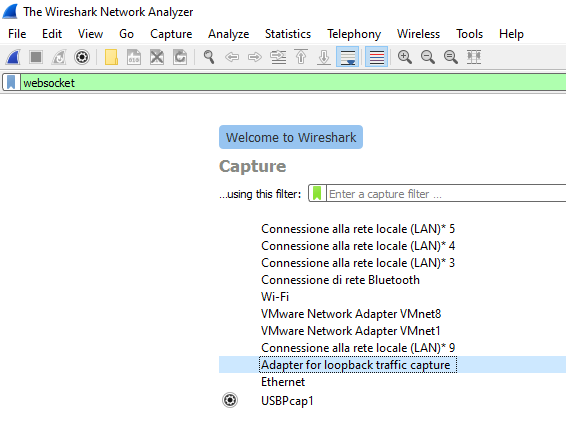
\includegraphics[width=\textwidth]{img/soluzioni_websocket-chat/wireshark-1.png}
	\end{figure}

	\noindent
	A questo punto, si aprono tre, quattro client. Quindi, si scrive l'URL localhost:4000 nel browser. Dato che il server non è in esecuzione, il browser non riesce a collegarsi al localhost:4000 poiché vede tale porta inutilizzata. Di conseguenza, il traffico catturato da Wireshark è inesistente.\newline

	\noindent
	Avviando il server, in automatico vedrà il collegamento dei 3/4 client avviati precedentemente. Di conseguenza, su Wireshark appariranno dei pacchetti corrispondenti al collegamento dei client al server:
	\begin{figure}[!htp]
		\centering
		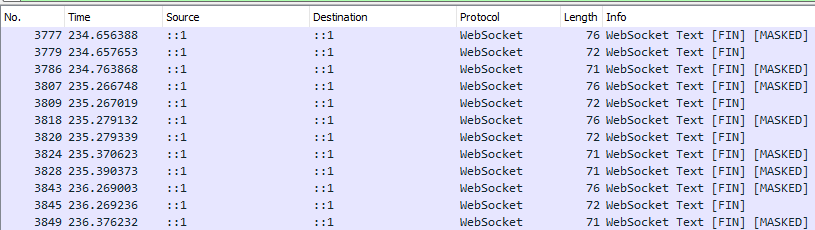
\includegraphics[width=\textwidth]{img/soluzioni_websocket-chat/wireshark-2.png}
	\end{figure}

	\noindent
	Cliccando su uno dei pacchetti con flag [MASKED] è possibile notare una cosa interessante riguardo il protocollo TCP. Ovvero, il numero di porta d'origine e destinazione. Per esempio, nell'immagine è possibile vedere come un client con porta 51021 (\emph{Source Port}) stia comunicando con il server sulla sua porta 4000 (\emph{Destination Port}):
	\begin{figure}[!htp]
		\centering
		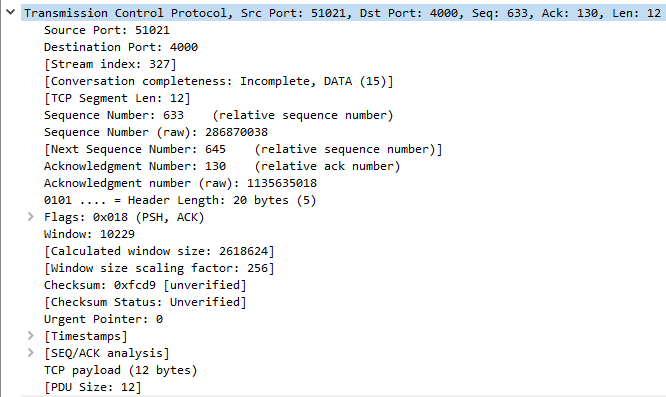
\includegraphics[width=\textwidth]{img/soluzioni_websocket-chat/wireshark-3.png}
	\end{figure}\newpage
	
	\noindent
	Adesso che è chiaro quale siano i client (quelli \dquotes{marchiati} con MASKED e il \href{https://en.wikipedia.org/wiki/WebSocket#Client_to_Server_Masking}{motivo per cui i messaggi sono mascherati è dovuto ad una questione di sicurezza}) e quale il server, è possibile vedere sulla colonna (la terza) di sinistra qual'è il tempo in cui ogni client comunica al server che è ancora vivo:
	\begin{figure}[!htp]
		\centering
		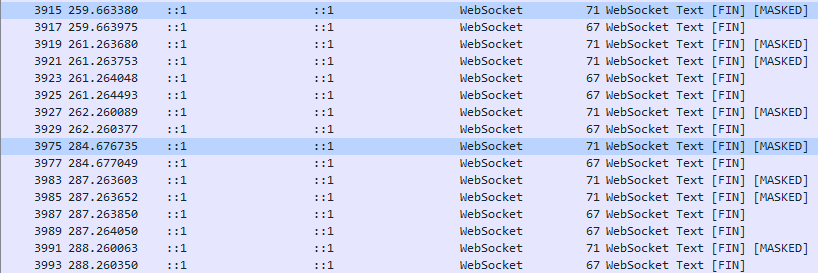
\includegraphics[width=\textwidth]{img/soluzioni_websocket-chat/wireshark-4.png}
	\end{figure}
	
	\noindent
	In questo caso, al tempo 259 il client con porta 51021 ha comunicato al server che è ancora vivo. Ovviamente il server ha risposto con un ACK e successivamente gli altri 3 client hanno comunicato al server la loro presenza. Al tempo 284, nuovamente il client con porta 51021 ricomunica al server che è ancora vivo (idem per gli altri). Si deduce che il client fa sapere al server che è ancora connesso ogni 25 secondi circa ($284-259=25$).\newline
	Documentazione ufficiale riguardo al Keep-Alive nel protocollo WebSocket: \url{https://websockets.readthedocs.io/en/stable/topics/timeouts.html}\newline
	RFC documentation: \url{https://www.rfc-editor.org/rfc/rfc6455#page-36}\newpage
	
	\noindent	
	\textcolor{Red3}{\textbf{\emph{\underline{Esercizio 2}}}}\newline
	
	\noindent
	Modificare il sorgente del codice per fare in modo che ad ogni utente connesso alla chat arrivi nella console il messaggio \dquotes{l'utente sta scrivendo...}.\newline
	
	\noindent
	NOTA: Lato client, bisogna spedire al server un evento apposito (ad es. \dquotes{typing}) quando l'utente scrive sulla tastiera (catturando l'evento di sistema \dquotes{keypress}). Lato server, la chiamata \textsf{webSocket.broadcast.emit('typing', data)} rilancia l'evento \dquotes{typing} a tutti i client connessi tranne che a quello dalla quale si è ricevuto il messaggio. Lato client infine gestire la ricezione de messaggio \dquotes{typing} che arriva dal server (si veda la gestione del messaggio \dquotes{UploadChat}).\newline
	
	\noindent	
	\textcolor{Green4}{\textbf{\emph{\underline{Soluzione esercizio 2}}}}\newline
	
	\noindent
	\lstinputlisting[language=JavaScript]{code/server_ex2.js}
	Il codice è rimasto lo stesso (paragrafo~\ref{codice Back-end server}), l'unica modifica effettuata è stata dalla riga 37 alla riga 39 in cui si impone al server di inoltrare il messaggio ricevuto, con tag \textsf{typing}, a tutti gli altri client eccetto il client mittente.\newpage
	
	\noindent
	\lstinputlisting[language=JavaScript]{code/chat_ex2.js}\newpage
	
	\noindent
	Il codice del front-end è rimasto pressoché identico (paragrafo~\ref{codice Front-end JavaScript}) tranne a due modifiche importanti:
	\begin{itemize}
		\item (20-26) Sull'elemento \textsf{message} della pagina HTML, si crea un evento. Nel momento in cui una lettera viene premuta, il client invierà il messaggio con tag \textsf{typing} al server, inserendo nel payload il nome del mittente (\textsf{sender.value}).
		
		\item (50-58) Alla ricezione dell'evento \textsf{typing} da parte del server, il client stamperà la scritta \textsf{typing...} .
	\end{itemize}
	
	\longline\newline
	
	\noindent	
	\textcolor{Red3}{\textbf{\emph{\underline{Esercizio 3}}}}\newline
	
	\noindent
	Modificare a piacimento il contenuto del file \textsf{public/index.html} e valutare l'impatto grafico.\newline
	
	\noindent	
	\textcolor{Green4}{\textbf{\emph{\underline{Soluzione esercizio 3}}}}\newline
	
	\noindent
	Una modifica che è possibile fare è l'aggiunta di un altro titolo con tag h2. Ovviamente i colori saranno in tema con quelli specificati dal file CSS (styles.css).\newline
	
	\longline\newline
	
	\noindent	
	\textcolor{Red3}{\textbf{\emph{\underline{Esercizio 4}}}}\newline
	
	\noindent
	Provare a collegarsi allo stesso server da browser presenti su diversi PC collegati in rete.\newline
	
	\noindent	
	\textcolor{Green4}{\textbf{\emph{\underline{Soluzione esercizio 4}}}}\newline
	
	\noindent
	In teoria dovrebbe funzionare anche con localhost, ma non ci sono riuscito per cui non posso fornire più di tante informazioni a riguardo.\newpage
	
	\subsection{Architetture orientate ai servizi (Service-Oriented Architecture, SOA)}
	
	Solitamente le applicazioni sono monolitiche, ovvero hanno un'interfaccia utente, la quale richiama delle funzionalità fornite da una serie di librerie linkate in un unico programma che è eseguito sulla macchina dell'utente.\newline
	
	\noindent
	Al giorno d'oggi esiste un altro approccio di sviluppo delle applicazioni che riguarda SOA. Le \textcolor{Red3}{\textbf{architetture orientate ai servizi}} (\emph{Service-Oriented Architecture}) riguarda lo sviluppo di applicazioni complesse attraverso la \textbf{combinazione di diversi programmi attraverso la rete}:
	\begin{itemize}
		\item L'interfaccia utente e qualche funzionalità di base sono eseguito sull'host dell'utente.
		\item Le funzionalità principali dell'applicazione sono fornite da programmi che sono eseguiti su uno o più server.
	\end{itemize}

	\noindent
	I \textcolor{Green4}{\textbf{vantaggi}} sono molteplici:
	\begin{itemize}
		\item \textbf{Potenza di calcolo e memoria} sono delegate al server;
		
		\item \textbf{Protezione} della proprietà intellettuale su \textbf{algoritmi} strategici;
		
		\item \textbf{Annullamento} della necessità di distribuire \textbf{aggiornamenti} software quando le modifiche riguardano solo il codice dei server;
		
		\item Nuovo modello economico: \textbf{pay per use};
		
		\item \textbf{Eliminazione della pirateria}.
	\end{itemize}
	Nonostante i grandi vantaggi che propone, c'è un \textbf{requisito fondamentale} che deve essere rispettato: \textbf{la presenza e l'affidabilità della rete}.
	
	\longline
	
	\subsubsection{Funzioni remote e webservice}
	
	\noindent
	Queste architetture \textbf{si basano} completamente sui servizi offerti, ovvero sulle \textbf{funzioni remote}.
	
	Le \textcolor{Red3}{\textbf{funzioni remote}} hanno il seguente funzionamento. Il \textbf{server espone una API}\footnote{Application program interface (API): insieme delle funzioni/metodi esposte da una certa libreria.}, \textbf{la quale descrive una serie di funzioni che il client} (\underline{non} il web browser) \textbf{può invocare}. Quindi, l'implementazione effettiva del \textbf{codice si trova \emph{server-side}}, mentre il codice che richiama una funzione specifica dell'API si trova \emph{client-side}.\newline
	
	\noindent
	In passato le tecnologie utilizzate per eseguire una chiamata a funzione remota erano scritte completamente in C e venivano chiamate \emph{Remote Procedure Call} (RPC). Dopodiché, vennero semplificate e programmate in Java tramite il \emph{Java Remote Method Invocation} (JAVA RMI). Successivamente, ci fu l'invenzione del \emph{Common Object Request Broker Architecture} (CORBA) che permise di scrivere e di far comunicare più client/server con linguaggi differenti.\newline
	Al giorno d'oggi, grazie all'approdo delle \textcolor{Red3}{\textbf{webservice}}, al protocollo HTTP/HTTPS e alla metodologia REST, le cose sono molto più semplici.
	
	\longline
	
	\subsubsection{Webservice basati su REST}\label{webservice basati su REST}
	
	I webservice basati su REST hanno molteplici vantaggi. Questa metodologia consente di poter \textbf{utilizzare due linguaggi di programmazione differenti \emph{client-side} e \emph{server-side}}. Anche l'\textbf{architettura può essere differente}. Questo grazie a due componenti fondamentali:
	\begin{itemize}
		\item \textbf{Funzione STUB}, \emph{client-side}: codifica dei parametri trasmessi e la decodifica dei valori di ritorno;
		
		\item \textbf{Componente SKELETON}, \emph{server-side}: decodificare l'input, eseguire il codice della libreria, codificare l'eventuale risultato e inviarlo al client.
	\end{itemize}
	La metodologia REST utilizza il protocollo HTTP/HTTPS. Il suo \textbf{servizio principale sono le chiamate remote e per farlo utilizza l'URL}, il quale è stato mappato (\emph{mapping}).
	
	I \textbf{parametri possono essere passati tramite URL}, metodo GET, oppure dopo l'header \textbf{nel payload}, con il metodo POST o PUT.\newline
	
	\noindent
	Alcune dei metodi HTTP più famosi in base ai quali viene eseguita una funzione specifica:
	\begin{itemize}
		\item \textbf{POST}: usato da funzioni che \textbf{creano un nuovo oggetto} sul server;
		
		\item \textbf{PUT}: usato da funzioni che \textbf{aggiornano un oggetto esistente} sul server;
		
		\item \textbf{GET}: usato da funzioni che \textbf{recuperano informazioni di un oggetto} sul server;
		
		\item \textbf{DELETE}: usato da funzioni che \textbf{distruggono un oggetto esistente} sul server;
	\end{itemize}
	Solitamente i \textbf{valori di ritorno} sono sotto forma di file JSON.\newline
	
	\noindent
	I \textcolor{Green4}{\textbf{vantaggi}} sono:
	\begin{itemize}
		\item A differenza di CORBA, il \textbf{webservice utilizza il protocollo HTTP/HTTPS}. Di conseguenza, elementi come \textbf{firewall o NAT sono già predisposti all'utilizzo} senza troppe complicazioni;
		
		\item Il \textbf{debugging è facilitato} (e quindi anche lo sviluppo di applicazioni) dall'utilizzo di contenuti testuali nelle transazioni, per esempio i file JSON.
	\end{itemize}\newpage
	
	\subsubsection{Breve introduzione ai file JSON}
	
	I file \textcolor{Red3}{\textbf{JSON}} sono dei file testuali nati con JavaScript, ma ad oggi supportati da quasi tutti i linguaggi di programmazione.\newline
	
	\noindent
	La sua è una \textbf{struttura gerarchica} facilmente leggibile da un umano e parserizzabile da un programma. La sua sintassi è semplice ed è formato da coppie \dquotes{\textsf{attributo:valore}}.\newline
	
	\noindent
	Possono essere presenti anche array, rappresentati con le parentesi quadre, e strutture dati, rappresentate con le parentesi graffe. Un \textcolor{Green4}{\textbf{esempio}} di formattazione JSON:
	\begin{lstlisting}
{"impiegati":[
	{
		"nome":"Giovanni",
		"cognome":"Rossi"
	},
	{
		"nome":"Anna",
		"cognome":"Bianchi"
	},
	{
		"nome":"Pietro",
		"cognome":"Verdi"
	}
]}\end{lstlisting}\newpage

	\subsection[\textcolor{Red3}{\textbf{Esercizi}} su webservice basati su REST]{Esercizi su webservice basati su REST}
	
	\subsubsection{Esercizio 1 - Analizzare server e \textsf{clientREST-GET}}
	
	Considerare la cartella \textsf{Webservice/}. Aprire il file serverHTTP-REST.c e analizzarne il contenuto. Compilarlo come al solito ed eseguirlo. Aprire il file clientREST-GET.c e analizzarne il contenuto. Compilarlo come al solito ed eseguirlo:
	\begin{itemize}
		\item Che parametri devo passare in linea di comando?
		\item Cosa si può vedere analizzando lo scambio di dati tramite Wireshark?
		\item Quale è la \emph{signature} della funzione calcolaSomma() sul server e sul client? Perché ha senso che siano uguali?
	\end{itemize}
	
	\noindent
	\textcolor{Green4}{\underline{\textbf{\emph{Soluzione}}}}\newline
	
	\noindent
	Il codice del server non viene commentato poiché quasi identico all'esercizio:
	\lstinputlisting[language=C]{code/serverHTTP-REST.c}\newpage
	
	\noindent
	Il codice del client è il seguente:
	\lstinputlisting[language=C]{code/clientREST-GET.c}
	Come si può vedere dal codice (24), il programma accetta solo un tipo di operazione, ovvero la somma, e due operandi numerici.\newline
	
	\noindent
	Analizzando i pacchetti con Wireshark, è possibile vedere una richiesta GET e i parametri inseriti tramite linea di comando.\newline
	
	\noindent
	Con \emph{signature} si intende la dichiarazione delle funzioni. In questo caso, il client esegue una richiesta inserendo i parametri ottenuti dalla linea di comando, all'interno di un URL. Successivamente, esegue una REST di tipo GET indirizzata al server, ottenuto grazie all'URL. Il server acquisisce i parametri dall'URL creato dal client e li utilizza per fare la somma nella sua funzione \textsf{calcolaSomma}.
	
	È ovvio che la \emph{signature} della funzione \textsf{calcoloSomma()} debba essere uguale. In caso contrario, potrebbe manifestarsi un risultato inesatto o un comportamento inaspettato.\newpage
	
	\subsubsection{Esercizio 2 - \textsf{ClientREST} in Java}
	
	Prendere in considerazione il file \textsf{ClientREST.java}. Dopo aver installato l'ambiente base di Java, si può compilare con \textsf{javac ClientREST.java} ed eseguire con \textsf{java ClientREST}. Il fatto che il server sia fatto in C e il client in Java è un problema? Perché?\newline
	
	\noindent
	\textcolor{Green4}{\underline{\textbf{\emph{Soluzione}}}}\newline
	
	\noindent
	Il client scritto in java è il seguente:
	\lstinputlisting[language=Java]{code/ClientREST.java}
	Grazie alle caratteristiche del protocollo REST (paragrafo~\ref{webservice basati su REST}), comunicare con il server non è un problema. Infatti, questa tecnologia si basa sul protocollo HTTP e non su quali linguaggi di programmazione sono scritti il client e il server. Di conseguenza, anche se il server fosse scritto in Python, non ci sarebbero problemi. L'unica cosa da tenere in considerazione è la \emph{signature} della funzione di calcolo della somma che deve rispettare i parametri.\newpage
	
	\subsubsection{Esercizio 3 - Modifica server per calcolare anche i numeri primi}\label{esercizio 3 - Modifica server per calcolare anche i numeri primi}
	
	Estendere il webservice \textsf{serverHTTP-REST.c} in modo che esponga un seconda servizio relativo al calcolo dei numeri primi compresi nell'intervallo $\left[min, max\right]$:
	\begin{itemize}
		\item Si tragga spunto dal programma \textsf{prime-number-interval.c}
	\end{itemize}
	Successivamente:
	\begin{itemize}
		\item Estendere il file \textsf{ClientREST.java} in modo da poter chiamare, a scelta, entrambe le funzionalità della nuova API.
		
		\item Provare il client con il calcolo dei numero primi compresi nell'intervallo $\left[1, 1000000\right]$: quanto tempi ci mette? Ho dovuto tradurre l'algoritmo dei numeri primi in Java? Perché?
	\end{itemize}
	
	\noindent
	\textcolor{Green4}{\underline{\textbf{\emph{Soluzione}}}}\newline
	
	\noindent
	Il codice del server viene modificato introducendo un nuovo metodo: \textsf{calcoloPrimi}. Tale funzione consente di calcolare i numeri primi e salvarli all'interno di una stringa già formattati pronti per essere inviati al client:
	\lstinputlisting[language=C]{code/serverHTTP-REST-ex3.c}\newpage
	
	\noindent
	Il codice del client viene modificato introducendo sempre un nuovo metodo, ma l'unica differenza è il salvataggio dei numeri nell'\textsf{ArrayList} locale (riga 95):
	\lstinputlisting[language=Java]{code/ClientREST-ex3.java}\newpage
	
	\subsubsection{Esercizio 4 - \textsf{ClientThreadREST} con thread concorrenti}
	
	Prendere in considerazione il file \textsf{clientThreadREST.java}:
	\begin{itemize}
		\item Esso invoca \textsf{calcolaSomma()} in 3 thread concorrenti
		
		\item Però la macchina su cui gira il server chiamato è la stessa e quindi non ci guadagno in prestazioni
		
		\item Come si dovrebbe modificare il codice in modo che le 3 invocazioni finiscano su 3 macchine diverse?
		
		\item Bisogna modificare anche il codice del server?
	\end{itemize}
	Si consideri il servizio che calcola i numeri primi nell'intervallo $\left[min, max\right]$ costruito nell'esercizio precedente:
	\begin{itemize}
		\item Si trovi un modo efficiente, sfruttando diversi server in rete, per calcolare i numeri primi tra 1 e 1000000
		
		\item Di quanto migliorano le prestazioni?
		
		\item Devo modificare anche il codice del server?
	\end{itemize}
	
	\noindent
	\textcolor{Green4}{\underline{\textbf{\emph{Soluzione}}}}\newline
	
	\noindent
	Il codice \textsf{clientThreadREST.java} è il seguente:
	\lstinputlisting[language=Java]{code/ClientThreadREST.java}
	Per eseguire il codice su tre macchine differenti, sarebbe necessario modificare l'URL di destinazione alle righe 12, 13 e 14. Al loro posto sarebbe necessario inserire l'indirizzo IP delle tre macchine differenti ed eseguire, su quest'ultime, il codice del \textsf{serverHTTP-REST.c}.\newpage
	
	\noindent
	Infine, si presenta di seguito un modo semplice ma efficiente per calcolare i numeri primi in un dato intervallo. Supponendo che nella rete ci siano diversi server che eseguano tale calcolo, si potrebbe eseguire il codice Java (qua sopra), aggiungendo il metodo di richiesta dei numeri primi come nell'esercizio precedente (paragrafo~\ref{esercizio 3 - Modifica server per calcolare anche i numeri primi}, pagina~\pageref{esercizio 3 - Modifica server per calcolare anche i numeri primi}), dichiarando tanti thread quanti sono i server e a ciascun thread imporre di richiedere al server un calcolo dei numeri primi in un intervallo diverso dagli altri.\newline
	
	\noindent
	Per \textbf{esempio}, si supponga che nella rete ci siano 5 server disponibili che hanno in esecuzione il server scritto nel linguaggio C. Se viene richiesto al client di calcolare un intervallo di numeri primi da 1 a $1'000'000$ effettuando una richiesta REST, il programma:
	\begin{enumerate}
		\item Dividerà il valore massimo per la quantità di server presenti nella rete, cioè 5 ($1'000'000 \div 5 = 200'000$);
		
		\item Creerà 5 istanze thread diverse assegnando loro un intervallo diverso:
		\begin{enumerate}
			\item 1° istanza thread, intervallo: $1 - 200'000$
			
			\item 2° istanza thread, intervallo: $200'001 - 400'000$
			
			\item 3° istanza thread, intervallo: $400'001 - 600'000$
			
			\item 4° istanza thread, intervallo: $600'001 - 800'000$
			
			\item 5° istanza thread, intervallo: $800'001 - 1'000'000$
		\end{enumerate}
	\end{enumerate}
	In questo modo il tempo per ottenere i risultati sarà ottimizzato di cinque volte rispetto a farlo eseguire su un solo server in un unico blocco.\newpage
	
	\subsection{Cloud computing}
	
	Il \textcolor{Red3}{\textbf{cloud computing}} è l'\textbf{accesso su richiesta}, via Internet, effettuato da un determinato host \textbf{verso le risorse informatiche}\footnote{Applicazioni, server fisici e virtuali, archiviazione di dati, strumenti di sviluppo, \emph{networking capabilities}, ecc.} \textbf{ospitate} da un \textbf{\emph{data center} remoto} gestito da un \textbf{\emph{provider} di servizi cloud}, chiamato CSP (\emph{Cloud Services Provider}).\newline
	
	\noindent
	In altre parole, è un gruppo di host in rete che forniscono servizi di calcolo e memorizzazione senza essere indirizzati o gestiti individualmente dagli utenti. Per \textcolor{Green4}{\textbf{esempio}}, i servizi più famosi sono: Amazon Web Service, Google Cloud, Microsoft Azure, Dropbox.\newline
	
	\noindent
	I \textbf{\emph{provider} di servizi cloud} (CSP) gestisce l'intero insieme di hardware e software. Esso mette a disposizione tali risorse a pagamento, con un costo che si differenzia a seconda della modalità scelta: può variare seconda del traffico/consumo generato oppure può variare con una modalità forfettaria.\newline
	
	\noindent
	Le tecnologie messe a disposizione forniscono dei servizi abbastanza importanti, tra cui:
	\begin{itemize}
		\item Consentire agli utenti una connessione perenne in rete;
		
		\item Dare a disposizione macchine virtuali (e.g. \href{https://azure.microsoft.com/it-it/resources/cloud-computing-dictionary/what-is-azure/}{Microsoft Azure}) per ottimizzare l'uso delle risorse hardware;
		
		\item Fornire WebService per far sfruttare le risorse di calcolo da remoto.
	\end{itemize}\newpage
	
	\subsubsection{Servizi offerti}
	
	I modelli di servizi cloud offerti sono molteplici, qua di seguito ne vengono presentati alcuni (i più famosi):
	\begin{itemize}
		\item \textcolor{Red3}{\textbf{\emph{On-site}}} oppure \textcolor{Red3}{\textbf{\emph{on-premise}}}, non è un vero e proprio servizio offerto da un CSP, ma si tratta di una \textbf{gestione personale}. In questo caso, l'\textbf{hardware è personale} e si trova in un posto di proprietà (per esempio a casa propria). La gestione è personale, quindi deve essere gestito qualsiasi aspetto:
		\begin{itemize}
			\item \textcolor{Green4}{\textbf{Pro:}} grande personalizzazione e libertà di scelta.
			\item \textcolor{Red4}{\textbf{Contro:}} non è disponibile la potenza di calcolo delle grandi aziende e la gestione non è semplice.
		\end{itemize}
		
		\item \textcolor{Red3}{\textbf{\emph{Infrastructure-as-a-Service} (IaaS)}}, viene concesso l'accesso alle risorse informatiche più fondamentali. Il servizio prevede l'\textbf{affitto di una macchina virtuale completamente vuota}, ovvero \textbf{senza sistema operativo o programmi addizionali}. La macchina risulta libera e pronta per ospitare un sistema operativo a scelta dell'utente ed eventuali applicazioni. Gli aspetti più importanti:
		\begin{itemize}
			\item \textcolor{Green4}{\textbf{Pro:}} libertà di installare qualsiasi sistema operativo ed applicazione.
			
			\item \textcolor{Red4}{\textbf{Contro:}} richieste abilità avanzate per gestire l'infrastruttura cloud a basso livello.
		\end{itemize}
		
		\item \textcolor{Red3}{\textbf{\emph{Platform-as-a-Service} (PaaS)}}, tra i servizi \textbf{più usati dagli sviluppatori software}, esso viene utilizzato principalmente per eseguire, sviluppare e gestire applicazioni senza il costo, la complessità e l'inflessibilità del mantenimento di una piattaforma. Quindi, viene concesso l'\textbf{affitto di un ambiente in cui è già presente un sistema operativo ed è possibile installare le proprie applicazioni}. Al giorno d'oggi, il servizio PaaS è implementato tramite una serie di virtualizzazioni sui server dei \emph{provider cloud services}, quindi vengono utilizzate tecnologie come Docker, Kubernetes, ecc. Gli aspetti più importanti:
		\begin{itemize}
			\item \textcolor{Green4}{\textbf{Pro:}} sistema \emph{ready-to-go}, adatto per gli sviluppatori che cercano una soluzione rapida per le loro applicazioni.
			
			\item \textcolor{Red4}{\textbf{Contro:}} impossibilità di operare a basso livello e necessità di adattarsi a sistemi già installati.
		\end{itemize}
		
		\item \textcolor{Red3}{\textbf{\emph{Software-as-a-Service} (SaaS)}}, è il servizio più ad alto livello ed è accessibile tramite un banale web browser. Viene \textbf{concesso un intero client desktop con tutti i servizi già a disposizione}. Quindi è possibile già trovare al loro interno: Web Server, Database Server, Broker per pub/sub. Gli aspetti più importanti:
		\begin{itemize}
			\item \textcolor{Green4}{\textbf{Pro:}} sistema con tutto il necessario per fare qualsiasi cosa. Risulta, ad oggi, uno dei servizi più utilizzati dalle aziende che vendono software commerciali.
			
			\item \textcolor{Red4}{\textbf{Contro:}} la macchina non ha un grado di personalizzazione paragonabile agli altri servizi.
		\end{itemize}
	\end{itemize}\newpage
	
	\begin{table}[!htp]
		\centering
		\begin{tabular}{@{} l | c c c c @{}}
			\toprule
			& On-site	& IaaS	& PaaS	& SaaS \\
			\midrule
			Applications	& \textcolor{Green4}{\ding{51}} & \textcolor{Green4}{\ding{51}} & \textcolor{Green4}{\ding{51}} & \textcolor{Red3}{\ding{55}} \\ [0.5em]
			Data			& \textcolor{Green4}{\ding{51}} & \textcolor{Green4}{\ding{51}} & \textcolor{Green4}{\ding{51}} & \textcolor{Red3}{\ding{55}} \\ [0.5em]
			Runtime			& \textcolor{Green4}{\ding{51}} & \textcolor{Green4}{\ding{51}} & \textcolor{Red3}{\ding{55}} 	& \textcolor{Red3}{\ding{55}} \\ [0.5em]
			Middleware		& \textcolor{Green4}{\ding{51}} & \textcolor{Green4}{\ding{51}} & \textcolor{Red3}{\ding{55}} 	& \textcolor{Red3}{\ding{55}} \\ [0.5em]
			O/S				& \textcolor{Green4}{\ding{51}} & \textcolor{Green4}{\ding{51}} & \textcolor{Red3}{\ding{55}} 	& \textcolor{Red3}{\ding{55}} \\ [0.5em]
			Virtualization	& \textcolor{Green4}{\ding{51}} & \textcolor{Red3}{\ding{55}} 	& \textcolor{Red3}{\ding{55}} 	& \textcolor{Red3}{\ding{55}} \\ [0.5em]
			Servers			& \textcolor{Green4}{\ding{51}} & \textcolor{Red3}{\ding{55}} 	& \textcolor{Red3}{\ding{55}} 	& \textcolor{Red3}{\ding{55}} \\ [0.5em]
			Storage			& \textcolor{Green4}{\ding{51}} & \textcolor{Red3}{\ding{55}} 	& \textcolor{Red3}{\ding{55}} 	& \textcolor{Red3}{\ding{55}} \\ [0.5em]
			Networking		& \textcolor{Green4}{\ding{51}} & \textcolor{Red3}{\ding{55}} 	& \textcolor{Red3}{\ding{55}} 	& \textcolor{Red3}{\ding{55}} \\ [0.5em]
			\bottomrule
		\end{tabular}
		\caption{Con \textcolor{Green4}{\ding{51}} si evidenzia cosa può gestire l'utente con quel servizio e con \textcolor{Red3}{\ding{55}} cosa viene gestito dal \emph{cloud service provider}.}
	\end{table}\newpage
	
	\subsubsection{Approfondimento: Function-as-a-Service (FaaS)}
	
	\textcolor{Red3}{\textbf{\emph{Function-as-a-Service} (FaaS)}} è un \textbf{servizio di \emph{cloud computing}} che consente ai clienti di \textbf{eseguire del codice in risposta al manifestarsi di determinati eventi}. Il grande vantaggio è l'assenza della gestione completa dell'infrastruttura, caratteristica, al contrario, tipica dei sistemi che devono gestire le applicazioni di microservizi.\newline
	
	\noindent
	Come accade anche negli altri servizi, l'hardware fisico, il sistema operativo e il web server, sono \textbf{gestiti completamente e \underline{automaticamente} dal \emph{cloud service provider}}. Questa caratteristica, consente agli sviluppatori di concentrarsi sul codice delle proprie applicazioni e non sulla gestione dell'infrastruttura che la circonda.\newline
	
	\noindent
	Alcuni tra i servizi commerciali più famosi:
	\begin{itemize}
		\item \href{https://aws.amazon.com/it/lambda/}{AWS Lambda}
		
		\item \href{https://cloud.google.com/functions?hl=it}{Google Cloud Functions}
		
		\item \href{https://www.ibm.com/it-it/cloud/functions}{IBM Cloud Functions based on Apache OpenWhisk}
		
		\item \href{https://azure.microsoft.com/it-it/products/functions/?ef_id=_k_064f86cb83d914979a22e2a5f86f67bb_k_&OCID=AIDcmmy6frl1tq_SEM__k_064f86cb83d914979a22e2a5f86f67bb_k_&msclkid=064f86cb83d914979a22e2a5f86f67bb}{Microsoft Azure Functions}
		
		\item \href{https://www.oracle.com/cloud/cloud-native/functions/}{Oracle Cloud Functions}
	\end{itemize}
	Quindi, per concludere:
	\begin{itemize}
		\item \textcolor{Green4}{\textbf{Pro:}}
		\begin{itemize}
			\item Niente preoccupazioni riguardo la gestione della struttura;
		
			\item Possibilità di concentrarsi al 100\% sullo sviluppo della propria applicazione e non sull'infrastruttura;
		
			\item Quantità elevata di servizi pronti all'uso;
		
			\item Assistenza tecnica da parte del team del \emph{cloud service provider}.
		\end{itemize}
		
		\item \textcolor{Red3}{\textbf{Contro:}}
		\begin{itemize}
			\item Decisioni limitate riguardo la gestione del proprio server, poiché gestito dal \emph{cloud service provider}. Per esempio, questioni sulla sicurezza o gestione del database;
			
			\item Necessario rispettare i limiti imposti dal server, come per esempio l'esecuzione di test. Quest'ultimi saranno più lenti dato che il server è in remoto sul cloud e non in locale;
			
			\item Il codice si deve adattare al server FaaS, a seconda delle funzionalità offerte.
		\end{itemize}
	\end{itemize}\newpage
	
	\section{Introduzione alla sicurezza}
	
	Per comprendere al meglio la sicurezza informatica, è necessario procedere a piccoli passi. Prima di tutto, ci sono delle domande da porsi:
	\begin{itemize}
		\item Quali risorse si vogliono proteggere? Risposta al paragrafo \ref{quali risorse si vogliono proteggere}
		\item Come vengono minacciate tali risorse? Risposta al paragrafo \ref{come vengono minacciate le risorse}
		\item Cosa è necessario fare per contrastare tali minacce? Risposta al paragrafo \ref{come contrastare le minacce}
	\end{itemize}

	\longline
	
	\subsection{Quali risorse si vogliono proteggere}\label{quali risorse si vogliono proteggere}
	
	Le risorse che solitamente si vogliono proteggere sono:
	\begin{itemize}
		\item Risorse \textbf{hardware}, come i sistemi, i componenti, dischi. In questo caso si parla di \textbf{sicurezza \dquotes{fisica}};
		
		\item Risorse \textbf{software}, come i sistemi operativi e gli applicativi;
		
		\item Risorse di \textbf{dati}, come file e database;
		
		\item Risorse di \textbf{rete}, come i collegamenti e gli apparati.
	\end{itemize}
	Per \textcolor{Red3}{\textbf{proteggere}} queste risorse è necessario \textbf{garantire le proprietà di}:
	\begin{itemize}
		\item Confidenzialità
		\item Integrità
		\item Disponibilità
		\item Autenticità
		\item Tracciabilità
	\end{itemize}
	
	\longline
	
	\subsubsection{Confidenzialità}
	
	Per \textcolor{Red3}{\textbf{confidenzialità}} si intende che \textbf{nessun utente deve poter ottenere o dedurre dal sistema informazioni che non è autorizzato a conoscere}. In questo caso ci sono due caratteristiche fondamentali:
	\begin{itemize}
		\item La \textbf{riservatezza dei dati}, ovvero le informazioni confidenziali non devono essere rilevate o rilevabili da utenti non autorizzati;
		
		\item La \textbf{privacy}, ovvero dare l'opportunità all'utente di controllare i dati che il sistema con cui sta interagendo può collezionare e memorizzare.
	\end{itemize}\newpage
		
	\subsubsection{Integrità}
	
	Per \textcolor{Red3}{\textbf{integrità}} si intende di \textbf{impedire l'alterazione diretta o indiretta delle informazioni, sia da parte di utente e processi non autorizzati, che a seguito di eventi accidentali}. Nel caso in cui i dati venissero alterati, sarebbe necessario fornire strumenti per poter verificare facilmente tale alterazione.\newline
	
	\noindent
	Anche qui ci sono due caratteristiche fondamentali:
	\begin{itemize}
		\item \textbf{Integrità dei dati}, ovvero le informazioni e i programmi possono essere modificati solo se autorizzati;
		
		\item \textbf{Integrità del sistema}, ovvero il sistema funzione e non è compromesso.
	\end{itemize}

	\longline
	
	\subsubsection{Disponibilità}
	
	Per \textcolor{Red3}{\textbf{disponibilità}} si intende la possibilità di \textbf{rendere disponibili a ciascun utente abilitato, le informazioni alle quali ha diritto di accedere, nei tempi e modi previsti}. Quindi in determinate condizioni o in un preciso istante o in un intervallo di tempo. Nei sistemi informatici, i requisiti di disponibilità includono caratteristiche di prestazioni e robustezza.
	
	\longline
	
	\subsubsection{Autenticità}
	
	Per \textcolor{Red3}{\textbf{autenticità}} si intende il \textbf{dovere da parte di ciascun utente di verificare l'autenticità delle informazioni}. Per esempio messaggi, mittenti e destinatari. Per garantire l'autenticità, si richiede di poter verificare se un'informazione è stata manipolata.
	
	\longline
	
	\subsubsection{Tracciabilità}
	
	Per \textcolor{Red3}{\textbf{tracciabilità}} si intende che le \textbf{azioni di un'entità devono essere tracciate in modo univoco così da supportare la non-ripudiabilità e l'isolamento della responsabilità}. Ad esempio, nessun utente deve poter ripudiare o negare in tempi successivi messaggi da lui spediti o firmati.\newpage
	
	\subsection{Come vengono minacciate le risorse} \label{come vengono minacciate le risorse}
	
	Le minacce compromettono le proprietà di confidenzialità, integrità e disponibilità. Per \textcolor{Green4}{\textbf{esempio}}:
	
	\begin{table}[!htp]
		\centering
		\begin{tabular}{@{} l p{9em} p{9em} p{9em} @{}}
			\toprule
			& Confidenzialità & Integrità & Disponibilità \\
			\midrule
			HW & & & Calcolatore rubato \\
			&&&\\
			SW & Copia non autorizzata & Eseguibile modificato & Eseguibili cancellati \\
			&&&\\
			Dati & Lettura non autorizzata & File modificati & File cancellati \\
			&&&\\
			Rete & Lettura messaggi inviati & Messaggi modificati/ritardati/duplicati & Messaggi distrutti, rete fuori uso \\
			\bottomrule
		\end{tabular}
	\end{table}
	
	\noindent
	Una \textcolor{Red3}{\textbf{minaccia}} è una \textbf{possibile violazione della sicurezza}. Mentre un \textcolor{Red3}{\textbf{attacco}} è una \textbf{violazione effettiva della sicurezza}. Gli \textbf{attacchi} possono essere:
	\begin{itemize}
		\item \textbf{Attivi}, tentativi di \textbf{alterare risorse o modificare il funzionamento} dei sistemi;
		
		\item \textbf{Passivi}, tentativi di \textbf{ottenere informazioni e utilizzarle} senza intaccare le risorse;
		
		\item \textbf{Interni}, iniziati da un'\textbf{entità interna} al sistema;
		
		\item \textbf{Esterni}, iniziati da un'\textbf{entità esterna}, tipicamente attraverso la rete.
	\end{itemize}\newpage
	
	\begin{figure}[!htp]
		\centering
		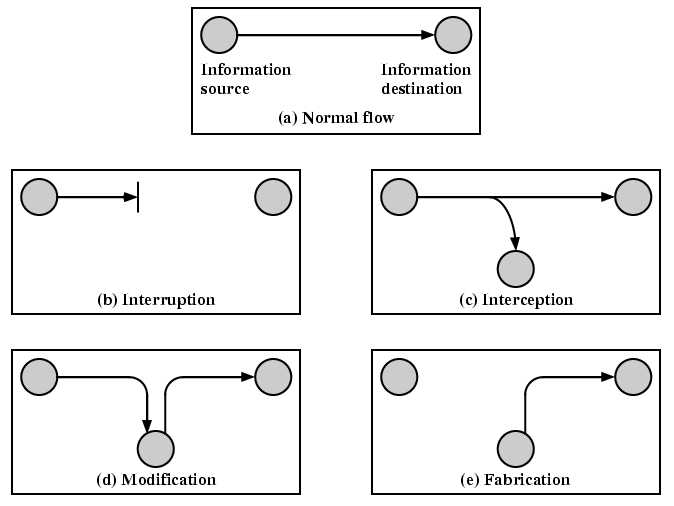
\includegraphics[width=\textwidth]{img/sicurezza/sicurezza.png}
		\caption{Esempi di attacchi.}
	\end{figure}

	\noindent
	Infine, esistono alcune classi di attacchi o minacce:
	\begin{itemize}
		\item \textbf{\emph{Disclosure}}, accesso non autorizzato alle informazioni
		
		\item \textbf{\emph{Deception}}, accettazione di dati falsi
		
		\item \textbf{\emph{Disruption}}, interruzione o prevenzione di operazioni corrette
		
		\item \textbf{\emph{Usurpation}} controllo non autorizzato di alcune parti del sistema
	\end{itemize}\newpage

	\subsection{Come contrastare le minacce}\label{come contrastare le minacce}
	
	Il contrasto delle minacce è la parte più difficile della sicurezza. Innanzitutto non esiste una risposta unica poiché dipende da una serie di fattori. Inoltre, le risorse cambiano con il tempo e quello che oggi è considerato come \dquotes{sistema sicuro}, un domani non potrebbe più esserlo.\newline
	
	\noindent
	\textbf{Durante la progettazione di sistemi} è necessario considerare la possibilità di \textbf{attacchi potenziali}. Quindi, l'obbiettivo è di considerare quali possibili attacchi un attaccante potrebbe mettere in atto. Nello sviluppo di meccanismi di difesa, è intelligente utilizzare delle \textbf{soluzioni contro-intuitive} così da complicare la vita ad eventuali malintenzionati.\newline
	
	\noindent
	I \textbf{meccanismi di sicurezza devono essere inseriti sia a livello fisico che a livello logico}, quindi protocollare. Tuttavia, nonostante il grande impegno che può esserci per sviluppare sistemi sicuri, la \textbf{sicurezza dipende anche dagli utenti}. Per esempio le informazioni possedute, come password, e la creazione/distribuzione/protezione di tali informazioni dovrebbero avere un occhio di riguardo.\newline
	
	\noindent
	Purtroppo sempre più spesso la \textbf{sicurezza viene vista come un impedimento e/o rallentamento} del normale funzionamento dei sistemi per una serie di motivi:
	\begin{itemize}
		\item Gli \textbf{amministratori conducono una battaglia no-stop contro gli attaccanti}, ai quali, a differenza dei difensori che devono eliminare \underline{qualsiasi} minaccia possibile, è sufficiente sfruttare una singola vulnerabilità;
		
		\item Dispendio di energie e forze senza un reale risultato tangibile. Questo si traduce in uno svantaggio e non in un beneficio. Ovviamente finché non accade un incidente di sicurezza...
		
		\item Sempre più elementi aggiuntivi al sistema.
	\end{itemize}\newpage
	
	\subsubsection{Principi fondamentali di progettazione della sicurezza}
	
	Nonostante anni di ricerca, è impossibile progettare sistema senza falle di sicurezza. Tuttavia, grazie ad un insieme di pratiche e regole è possibile creare un sistema molto difficile da attaccare con successo. Queste \textbf{regole} vengono chiamate \textcolor{Red3}{\textbf{principi fondamentali di progettazione della sicurezza}}:
	\begin{itemize}
		\item \textbf{Aspetti economici dei meccanismi}, la progettazione delle misure di sicurezza deve essere il più semplice possibile, sia da implementare che da verificare;
		
		\item \textbf{\emph{Fail-safe default}}, i comportamenti non specificati devono prevedere un default sicuro, ad esempio i permessi di accesso;
		
		\item \textbf{Progettazione aperta} è preferibile rispetto al codice segreto;
		
		\item \textbf{Tracciabilità delle operazioni}, così che qualsiasi operazione può essere ricostruita e il sistema ripristinato;
		
		\item \textbf{Separazione dei privilegi} dalle risorse create da ciascun utente e da quelle critiche;
		
		\item \textbf{Separazione delle funzionalità}, ovvero la distinzione dei ruoli nei diversi punti del sistema fisico e logico;
		
		\item \textbf{Isolamento dei sottosistemi}, ovvero un sistema compromesso non dovrebbe compromettere gli altri;
		
		\item \textbf{Modularità}, quindi meccanismi di sicurezza indipendenti, sostituibili e riusabili.
	\end{itemize}\newpage
	
	\subsubsection{Politiche di sicurezza e meccanismi}
	
	Una \textcolor{Red3}{\textbf{politica di sicurezza}} è un'indicazione di \textbf{cosa è permesso e di cosa non è concesso}. Le regole riguardano i dati, le operazioni possibili, gli utenti singoli e i profili.\newline
	
	\noindent
	Un \textcolor{Red3}{\textbf{meccanismo di sicurezza}} è un metodo (strumento/procedura) per garantire una politica di sicurezza.\newline
	
	\noindent
	Quindi, data l'unione di queste due definizione, si dice: data una politica che distingue le azioni sicure da quelle non sicure, i meccanismi di sicurezza \textbf{prevengono}, \textbf{scoprono} o \textbf{recupero} da un attacco.
	\begin{itemize}
		\item \textbf{Prevenzione} di un attacco, ovvero il meccanismo di sicurezza deve rende impossibile l'attacco. Spesso l'adozione di questa politica interferisce con il sistema al punto da renderlo scomodo da usare. Per \textcolor{Green4}{\textbf{esempio}}, la richiesta di password come modo di autenticazione.
		
		\item \textbf{Scoperta} di un attacco, quindi il meccanismo di sicurezza è in grado di scoprire che un attacco è in corso. È \textbf{utile} quando:
		\begin{itemize}
			\item Non è possibile prevenire l'attacco;
			\item È necessario valutare le misure preventive.
		\end{itemize}
		Solitamente vengono monitorate le risorse del sistema, cercando eventuali tracce di attacchi.
		
		\item \textbf{Recupero} da un attacco. Questa politica è possibile applicarla in due modi diversi:
		\begin{enumerate}
			\item \textbf{Fermare l'attacco} e recuperare o ricostruire la situazione prima dell'attacco, per esempio con un backup;
			
			\item \textbf{Continuare a far funzionare il sistema correttamente durante l'attacco}, in gergo viene chiamata \emph{fault-tolerant}.
		\end{enumerate}
	\end{itemize}
	Degli \textcolor{Green4}{\textbf{esempi}} di meccanismi (specifici) di sicurezza sono: la \textbf{crittografia}, cioè la trasformazione dei dati in un formato non facilmente comprensibile da un essere umano, la \textbf{firma digitale}, usata per provare la sorgente, l'\textbf{autenticazione e controllo degli accessi}, come la gestione dei diritti degli utenti rispetto le risorse. I meccanismi generali possono essere il rilevamento degli eventi, la gestione degli Audit (\href{https://it.wikipedia.org/wiki/Audit}{Wikipedia}) o le Recovery (\href{https://www.cybersecurity360.it/soluzioni-aziendali/cyber-event-recovery-strutturare-un-piano-dazione-per-ripristinare-dati-sistemi-e-servizi/}{CyberSecurity360}).\newpage
	
	\subsubsection{Ottenere un sistema sicuro}
	
	Per ottenere un \textcolor{Red3}{\textbf{sistema sicuro}}, i primi passi sono uno sviluppo consapevole. È dunque necessario seguire le seguenti \textbf{fasi}:
	\begin{enumerate}
		\item \textbf{Specifica}, descrive il funzionamento del sistema desiderato e avere una visione d'insieme;
		\item \textbf{Progetto}, tradurre le specifiche in componenti che le implementano ed elencare le loro caratteristiche;
		\item \textbf{Implementazione}, creare il sistema vero e proprio che soddisfi le specifiche.
	\end{enumerate}
	Durante queste fasi è \underline{fondamentale} continuare a verificare la correttezza dell'implementazione.\newline
	
	\noindent
	Inoltre, è importante \textbf{considerare alcune scelte implementative} inevitabili durante la progettazione di un sistema:
	\begin{itemize}
		\item \textbf{Analizzare} i \textbf{costi-benefici} dell'implementazione della \textbf{sicurezza} e dei suoi meccanismi;
		
		\item \textbf{Analizzare i rischi} in caso di attacchi e gli eventuali danni/perdite che possono causare;
		
		\item \textbf{Aspetti legali} riguardanti la sicurezza e la privacy ed eventuali \textbf{aspetti morali};
		
		\item \textbf{Analizzare i problemi organizzativi}, infatti l'implementazione di meccanismi di sicurezza, come detto nei paragrafi precedenti, potrebbe creare situazioni di difficoltà per gli utenti che utilizzano il sistema. Questo si potrebbe tradurre nell'aumento di perdite invece di utili;
		
		\item \textbf{Aspetti comportamentali} delle persone coinvolte.
	\end{itemize}
	
	\newpage


%%%%%%%%%%%%%%%%%%%%%%%%%%%%%%%%%%%%%%%%%%%%%%%%%%%%%%%%%%%%%%%%%%%%%%%%%%%%%%%%%%%%%%%%%%%%%%%%%%%%%%%%%%%%%%%%%%%%%%%%%%%%%%%%%%%%%%%%%%%%%%%%%%%%%%%%%%%%%%%%%%%%%%%%%%%%%%%%%%%%%%%%%%%%%%%%%%%%%%%%%%%%%%%%%%%%%%%%%%%%%%%%%%%%%%%%%%%%%%%%%%%%%%%%
%%%%%%%%%%%%%%%%%%%%%%%%%%%%%%%%%%%%%%%%%%%%%%%%%%%%%%%%%%%%%%%%%%%%%%%%%%%%%%%%%%%%%%%%%%%%%%%%%%%%%%%%%%%%%%%%%%%%%%%%%%%%%%%%%%%%%%%%%%%%%%%%%%%%%%%%%%%%%%%%%%%%%%%%%%%%%%%%%%%%%%%%%%%%%%%%%%%%%%%%%%%%%%%%%%%%%%%%%%%%%%%%%%%%%%%%%%%%%%%%%%%%%%%%%%%%%%%%%%%%%%%%%%%%%%%%%%%%%%%%%%%%%%%%%%%%%%%%%%%%%%%%%%%%%%%%%%%%%%%%%%%%%%%%%%%%%%%%%%%%%%%%%%%%%%%%%%%%%%%%%%%%%%%%%%%%
%%%%%%%%%%%%%%%%%%%%%%%%%%%%%%%%%%%%%%%%%%%%%%%%%%%%%%%%%%%%%%%%%%%%%%%%%%%%%%%%%%%%%%%%%%%%%%%%%%%%%%%%%%%%%%%%%%%%%%%%%%%%%%%%%%%%%%%%%%%%%%%%%%%%%%%%%%%%%%%%%%%%%%%%%%%%%%%%%%%%%%%%%%%%%%%%%%%%%%%%%%%%%%%%%%%%%%%%%%%%%%%%%%%%%%%%%%%%%%%%%%%%%%%%%%%%%%%%%%%%%%%%%%%%%%%%%%%%%%%%%%%%%%%%%%%%%%%%%%%%%%%%%%%%%%%%%%%%%%%%%%%%%%%%%%%%%%%%%%%%%%%%%%%%%%%%%%%%%%%%%%%%%%%%%%%%%%%%%%%%%%%%%%%%%%%%%%%%%%%%%%%%%%%%%%%%%%%%%%%%%%%%%%%%%%%%%%%%%%%%%%%%%%%%%%%%%%%%%%%%%%%%%%%%%%%%%%%%%%%%%%%%%%%%%%%%%%%%
%%%%%%%%%%%%%%%%%%%%%%%%%%%%%%%%%%%%%%%%%%%%%%%%%%%%%%%%%%%%%%%%%%%%%%%%%%%%%%%%%%%%%%%%%%%%%%%%%%%%%%%%%%%%%%%%%%%%%%%%%%%%%%%%%%%%%%%%%%%%%%%%%%%%%%%%%%%%%%%%%%%%%%%%%%%%%%%%%%%%%%%%%%%%%%%%%%%%%%%%%%%%%%%%%%%%%%%%%%%%%%%%%%%%%%%%%%%%%%%%%%%%%%%%%%%%%%%%%%%%%%%%%%%%%%%%%%%%%%%%%%%%%%%%%%%%%%%%%%%%%%%%%%%%%%%%%%%%%%%%%%%%%%%%%%%%%%%%%%%%%%%%%%%%%%%%%%%%%%%%%%%%%%%%%%%%
	\section{Analisi di rete con Wireshark e da linea di comando}
	
	\subsection{Introduzione agli analizzatori di rete}
	
	Esistono diversi \textbf{strumenti software che consentono di analizzare i pacchetti} che arrivano alla propria interfaccia di rete:
	\begin{itemize}
		\item \textbf{TCDUMP} tool da linea di comando per sistemi operativi Linux;
		
		\item \textbf{WinDump} tool da linea di comando per sistemi operativi Windows;
		
		\item \textbf{Wireshark} tool sia da linea di comando che da GUI per sistemi operativi Linux, Windows e MacOS.
	\end{itemize}
	Tutti gli \textbf{strumenti di rete si basano sulla libreria} del linguaggio programmazione C, chiamata \textcolor{Red3}{\textbf{\textsf{libpcap}}}. Le sue funzionalità sono tre:
	\begin{enumerate}
		\item Cercare e trovare interfacce di rete;
		
		\item Gestione avanzata di filtri di cattura;
		
		\item Gestione degli errori e statistiche di cattura.
	\end{enumerate}
	
	\longline
	
	\subsubsection{Sniffing e la motivazione del \textsf{sudo}}\label{sniffing e la motivazione del sudo}
	
	Con il termine \textcolor{Red3}{\textbf{\emph{sniffing}}} viene intesa l'abilità del software, in questo caso Wireshark, di \textbf{catturare i pacchetti in arrivo e in partenza} dalla propria interfaccia di rete. Esistono due tipi di \emph{sniffing}:
	\begin{itemize}
		\item \emph{Sniffing} all'interno di \textcolor{Red3}{\textbf{reti non-switched}}. Come accade, per esempio, nelle \textbf{reti WiFi}, tutte le schede di rete dei PC collegati al router ricevono tutti i pacchetti, sia i propri sia quelli destinati ad altri.
		
		In questo caso, lo \emph{sniffing} consente di \textbf{catturare sia i pacchetti destinati al dispositivo che sta eseguendo questa operazione, sia i pacchetti di cui non è il destinatario}. Per eseguire questa operazione è necessario avviare Wireshark in modalità amministratore (comando \textsf{sudo} su Linux). Questo perché a priori l'\textbf{interfaccia di rete scarta i pacchetti a cui non è interessato}, mentre con Wireshark viene attivata la \textcolor{Red3}{\textbf{modalità promiscua}} che \textbf{consente di bypassare il sistema operativo e interrogare direttamente la CPU per salvare tutti i pacchetti in entrata e in uscita}. La modalità promiscua viene disattivata dal sistema operativo per motivi di \emph{performance}. Infatti, se fosse sempre attiva, il sistema operativo avrebbe un carico di lavoro talmente alto sulla CPU che calerebbero le prestazioni generali del sistema.
		
		\item \emph{Sniffing} all'interno di \textcolor{Red3}{\textbf{reti Ethernet switched}}. In questo caso, l'apparato centrale della rete (\emph{switch}), si preoccupa di \textbf{inoltrare su ciascuna porta solo il traffico destinato ai dispositivi collegati a quella porta}. Di conseguenza, ciascuna interfaccia di rete riceve solo i pacchetti destinati a lei (o multicast/broadcast).
		
		In altre parole, la \textbf{modalità promiscua \underline{non} consente la cattura di pacchetti di altre schede di rete}.
	\end{itemize}\newpage

	\subsection{Interfaccia grafica di Wireshark}
	
	Come specificato nel paragrafo~\ref{sniffing e la motivazione del sudo}, Wireshark necessita di essere avviato con la modalità amministratore (o \textsf{sudo} su Linux).
	
	Una volta avviato, la schermata iniziale sarà la seguente. Al centro sono presenti una serie di voci in cui vengono indicati i vari dispositivi di rete su cui è possibile ascoltare il traffico. Oltre all'interfaccia Wi-Fi (se presente sulla macchina), è possibile trovare interfacce del tipo bluetooth, ethernet (LAN), USB e interfacce di rete delle macchine virtuali.
	\begin{figure}[!htp]
		\centering
		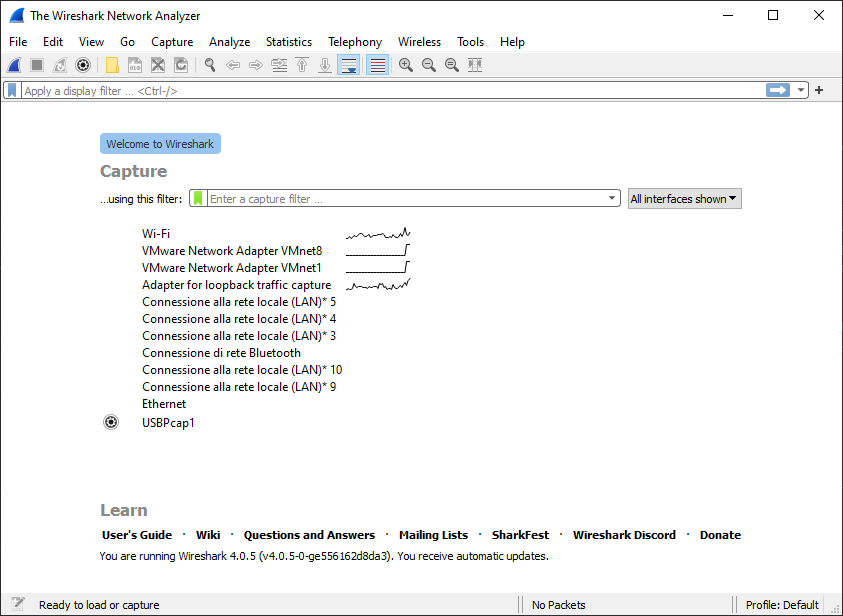
\includegraphics[width=\textwidth]{img/wireshark/grafica-wireshark-1.png}
		\caption{Schermata iniziale di Wireshark.}
	\end{figure}\newpage

	\subsubsection{Sniffing della rete}

	Cliccando su una delle interfacce, il software inizierà ad ascoltare il traffico di pacchetti nella rete. La grafica si presenta nel seguente modo e con i seguenti colori:
	\begin{figure}[!htp]
		\centering
		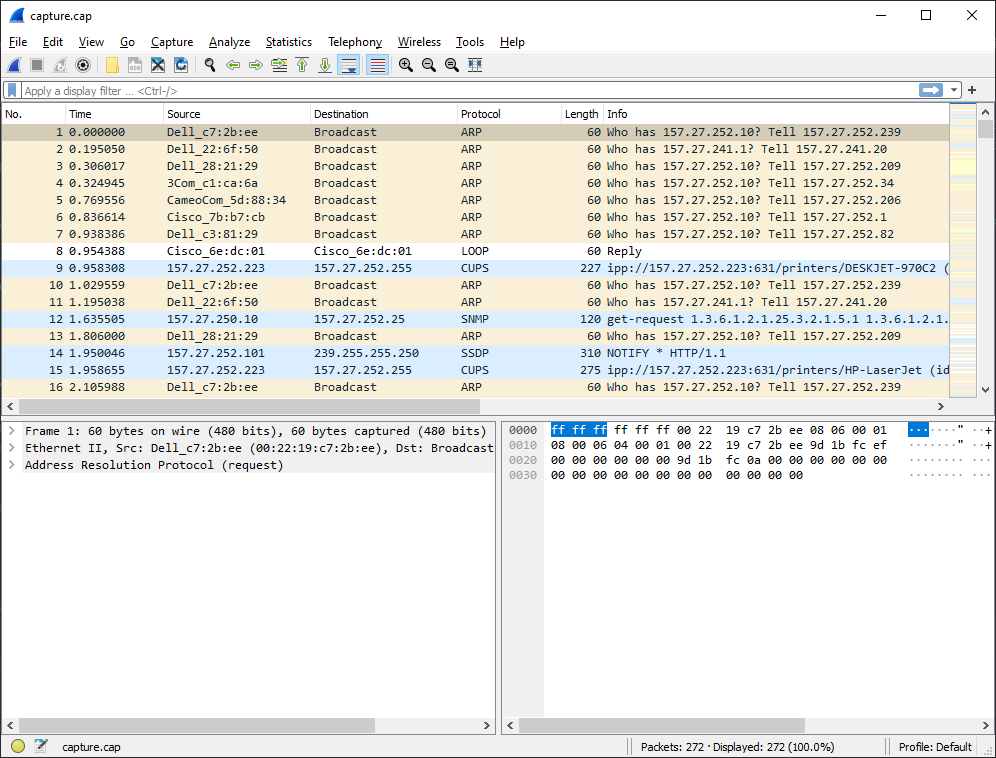
\includegraphics[width=\textwidth]{img/wireshark/grafica-wireshark-2.png}
		\caption{Schermata di \emph{sniffing} nella rete.}
	\end{figure}

	\longline
	
	\subsubsection{Applicazione dei filtri}\label{applicazione dei filtri}
	
	Data la grande mole di pacchetti che possono presentarsi durante lo \emph{sniffing}, Wireshark dà la possibilità di applicare una serie di filtri (la serie di comandi che è possibile utilizzare: \href{https://www.wireshark.org/docs/man-pages/wireshark-filter.html}{documentazione ufficiale}). Essi possono essere applicati scrivendo il relativo comando nella barra in alto in cui è scritto \dquotes{\textsf{Apply a display filter ...}}. Per \textcolor{Green4}{\textbf{esempio}} è possibile ricercare un protocollo scrivendolo nella barra (se quest'ultima viene evidenziata di verde, il comando è corretto, altrimenti viene evidenziata di rosso per segnalare un'inesattezza nel comando).
	\begin{figure}[!htp]
		\centering
		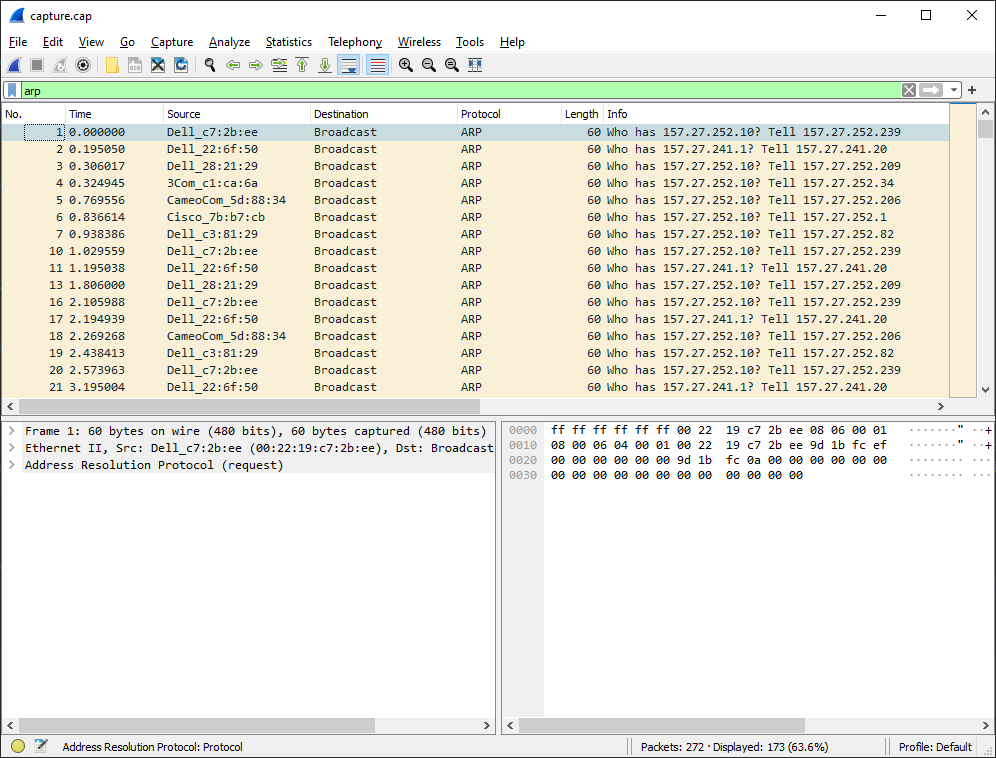
\includegraphics[width=\textwidth]{img/wireshark/grafica-wireshark-3.png}
		\caption{Applicazione corretta di un filtro.}
		\vspace{2em}
		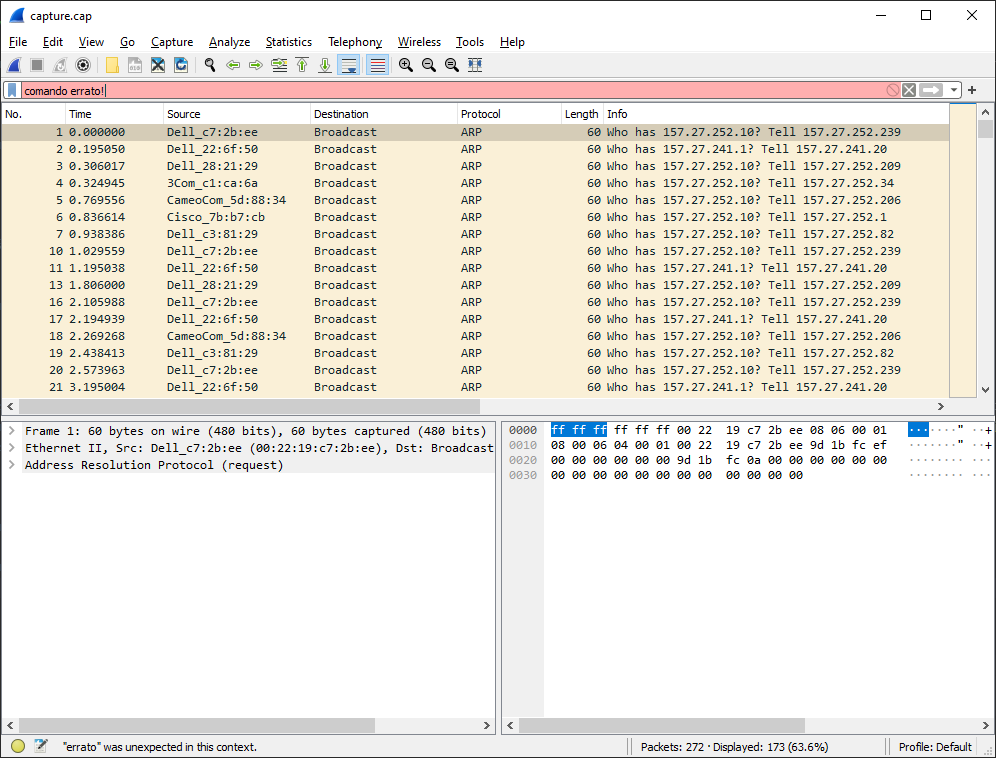
\includegraphics[width=\textwidth]{img/wireshark/grafica-wireshark-4.png}
		\caption{Applicazione errata di un filtro.}
	\end{figure}\newpage

	\subsubsection{Seguire il flusso di una conversazione}
	
	È possibile seguire il flusso dati della \dquotes{conversazione} di un pacchetto. Per farlo è necessario cliccare sul pacchetto interessato, andare nella barra degli strumenti e cliccare \emph{Analyze} $\rightarrow$ \emph{Follow} e selezionare il protocollo interessato. Per \textcolor{Green4}{\textbf{esempio}}, nella seguente conversazione viene seguito il protocollo UDP.
	
	\begin{figure}[!htp]
		\centering
		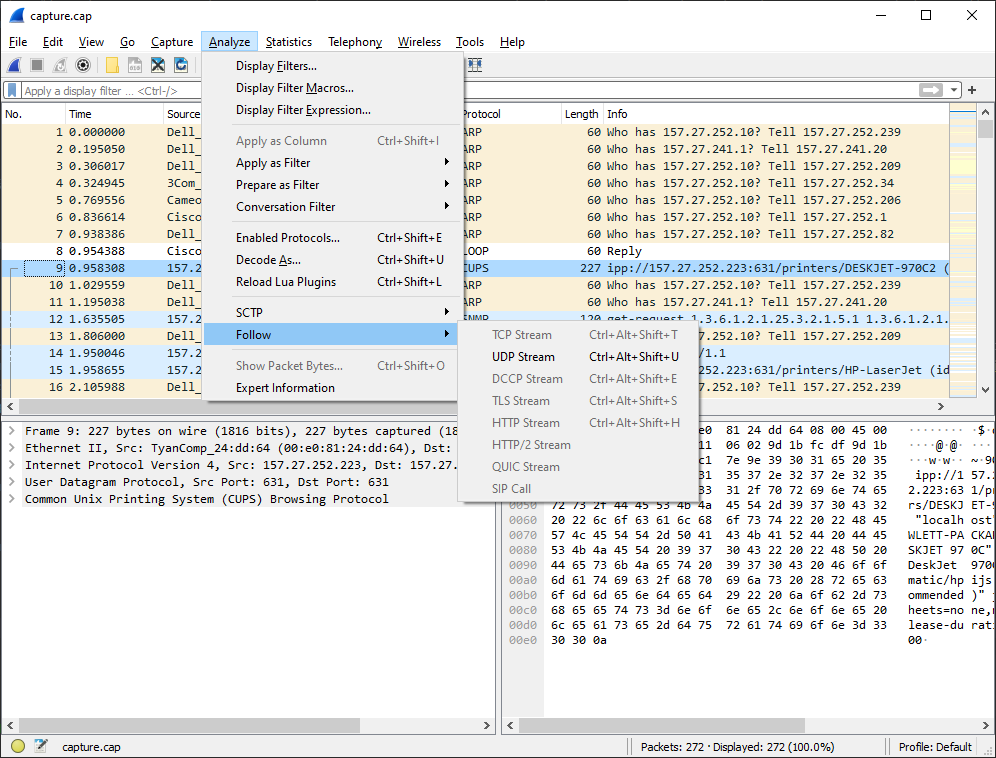
\includegraphics[width=\textwidth]{img/wireshark/grafica-wireshark-5.png}
		\caption{Analisi del flusso di un pacchetto 1 di 2.}
		\vspace{2em}
		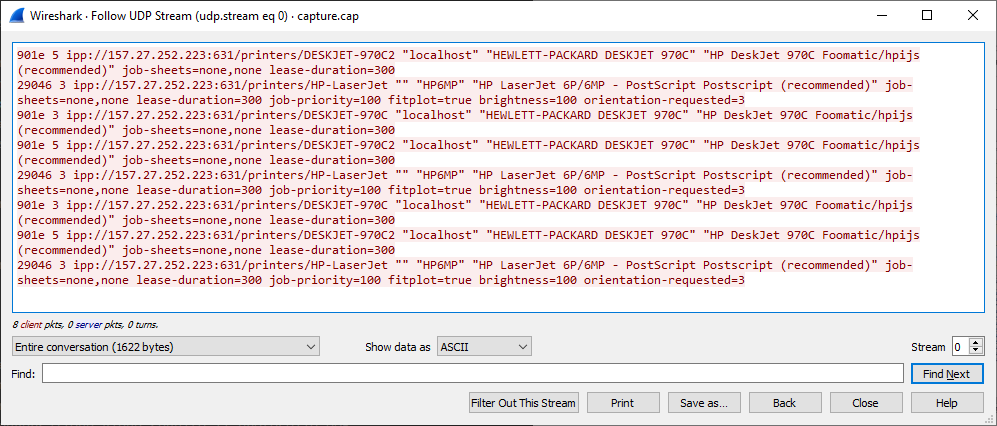
\includegraphics[width=\textwidth]{img/wireshark/grafica-wireshark-6.png}
		\caption{Analisi del flusso di un pacchetto 2 di 2.}
	\end{figure}\newpage

	\subsection{Comando \textsf{ping}}
	
	Il comando \textcolor{Red3}{\textsf{ping}} consente di \textbf{verificare la raggiungibilità di un computer connesso alla rete e il relativo Round Trip Time} (RTT)\footnote{Tempo che intercorre dalla partenza del pacchetto inviato fino al ritorno della risposta.}. Per questa operazione viene utilizzato il protocollo ICMP (Internet Control Message Protocol) che è un servizio per trasmettere informazioni riguardanti malfunzionamenti, informazioni di controllo o messaggi tra vari componenti di una rete di calcolatori.
	
	\begin{figure}[!htp]
		\centering
		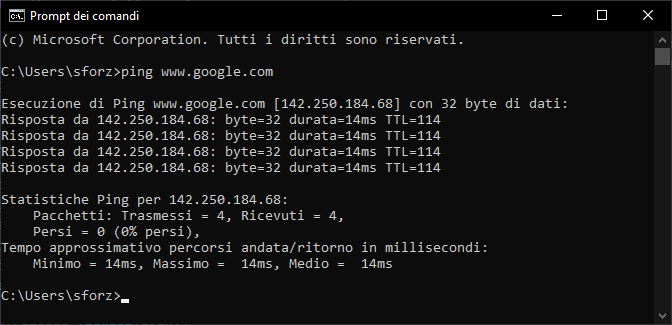
\includegraphics[width=\textwidth]{img/altri-strumenti/ping.png}
		\caption{Esempio di esecuzione del comando \textsf{ping}.}
	\end{figure}\newpage
	
	\subsection{Comando \textsf{traceroute} (\textsf{tracert} Windows)}
	
	Il comando \textcolor{Red3}{\textsf{traceroute}} (\textsf{tracert} in Windows) è un semplice strumento per \textbf{tracciare il precorso che un pacchetto segue dalla sorgente alla destinazione}. Il comando mostra un elenco di tutte le interfacce dei router che il pacchetto attraversa finché non raggiunge la destinazione. Per questioni di sicurezza, alcuni nodi possono non essere visibili tramite il comando \textsf{traceroute}, questo per evitare che venga resa nota la struttura della rete.
	
	\begin{figure}[!htp]
		\centering
		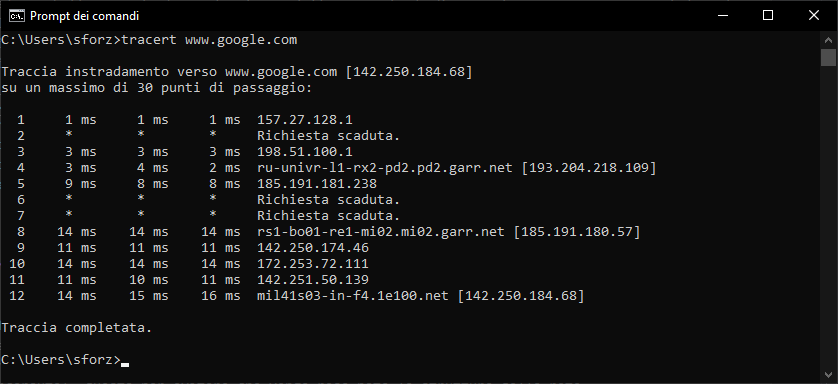
\includegraphics[width=\textwidth]{img/altri-strumenti/traceroute.png}
		\caption{Esempio di esecuzione del comando \textsf{tracert} su Windows (\textsf{traceroute} su Linux).}
	\end{figure}\newpage

	\subsection{Comando \textsf{nslookup}}
	
	Il comando \textcolor{Red3}{\textsf{nslookup}} consente di \textbf{effettuare un'interrogazione ai server DNS (Domain Name System)\footnote{Sistema di server organizzato gerarchicamente per la gestione del namespace.} per poter ottenere da un hostname il relativo indirizzo IP, o viceversa}. Esso può essere utilizzato in modalità: \textbf{interattiva} o \textbf{non interattiva}.\newline
	
	\noindent
	La \textbf{modalità interattiva} consente di \textbf{effettuare più interrogazioni} e visualizza i singoli risultati. Viene attivata eseguendo il comando senza parametri.
	
	\begin{figure}[!htp]
		\centering
		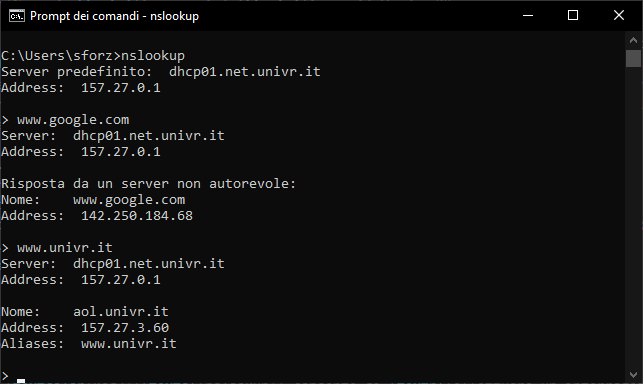
\includegraphics[width=\textwidth]{img/altri-strumenti/nslookup1.png}
		\caption{Esempio di esecuzione del comando \textsf{nslookup} in modalità interattiva.}
	\end{figure}

	\noindent
	La \textbf{modalità \underline{non} interattiva} consente di \textbf{effettuare una sola interrogazione} visualizzandone il risultato. Viene attivata se viene inserito un parametro che corrisponde ad un \emph{host-to-find}.
	
	\begin{figure}[!htp]
		\centering
		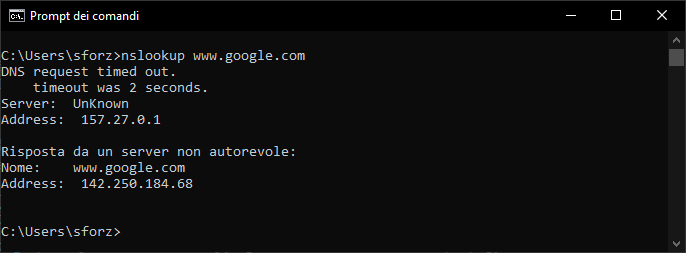
\includegraphics[width=\textwidth]{img/altri-strumenti/nslookup2.png}
		\caption{Esempio di esecuzione del comando \textsf{nslookup} in modalità \underline{non} interattiva.}
	\end{figure}\newpage
	
	\subsection{Comando \textsf{ifconfig} (\textsf{ipconfig} Windows)}\label{comando ifconfig (ipconfig Windows)}
	
	Il comando \textcolor{Red3}{\textsf{ifconfig}} (\textsf{ipconfig} in Windows) è utilizzato per \textbf{configurare e controllare un'interfaccia di rete TCP/IP} da riga di comando. La sua esecuzione con il parametro \dquotes{\textsf{-a}} stampa su terminale le informazioni di tutte le interfacce di rete.\newline
	
	\noindent
	Vengono stampate molteplici interfacce di rete, ma tra queste le più famose sono:
	\begin{itemize}
		\item \textsf{eth0} è la prima interfaccia Ethernet;
		
		\item \textsf{lo} è l'interfaccia \emph{loopback}, sempre presente. È \dquotes{speciale} poiché il sistema la utilizza per comunicare con sé stesso;
		
		\item \textsf{wlan0} è il nome della prima interfaccia di rete Wireless del sistema.
	\end{itemize}
	
	\begin{figure}[!htp]
		\centering
		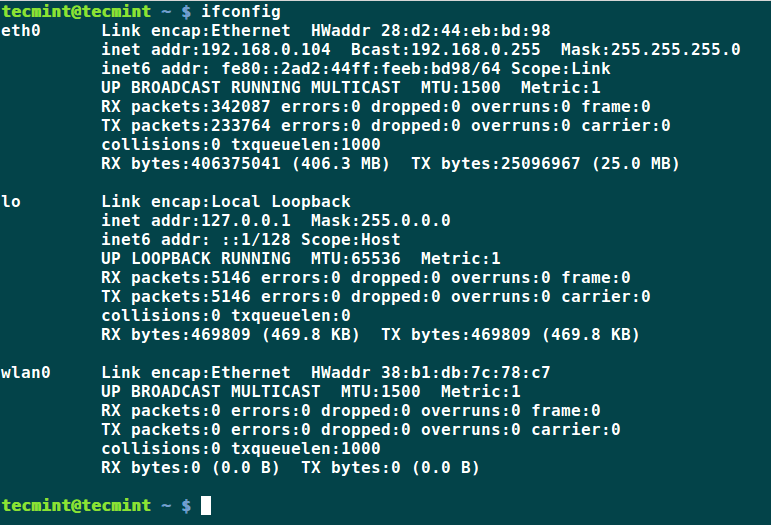
\includegraphics[width=\textwidth]{img/altri-strumenti/ifconfig.png}
		\caption{Esempio di esecuzione del comando \textsf{ifconfig} su Linux.}
	\end{figure}\newpage

	\subsection{Comando \textsf{route} (\textsf{route PRINT} Windows)}
	
	Il comando \textcolor{Red3}{\textsf{route}} (\textsf{route PRINT} su Windows) è utilizzato per \textbf{visualizzare e modificare le tabelle di routing}. L'esecuzione consente di visualizzare la tabella di routing dell'host.

	\begin{figure}[!htp]
		\centering
		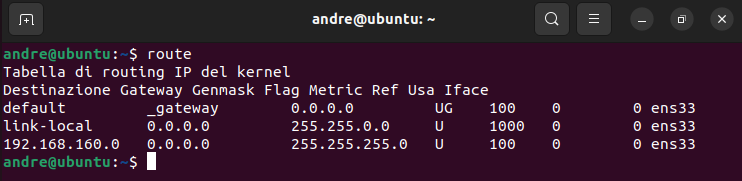
\includegraphics[width=\textwidth]{img/altri-strumenti/route.png}
		\caption{Esempio di esecuzione del comando \textsf{ifconfig} su Linux.}
	\end{figure}

	\longline	

	\subsection{Comando \textsf{whois}}
	
	Il comando \textsf{whois} consente, mediante l'interrogazione di database server da parte di un client, di \textbf{stabilire il nome privato, o dell'azienda, o dell'ente, al quale è intestato un determinato indirizzo IP o uno specifico DNS}. Solitamente vengono mostrate anche informazioni riguardanti l'intestatario, data di registrazione e data di scadenza.
	
	\begin{figure}
		\centering
		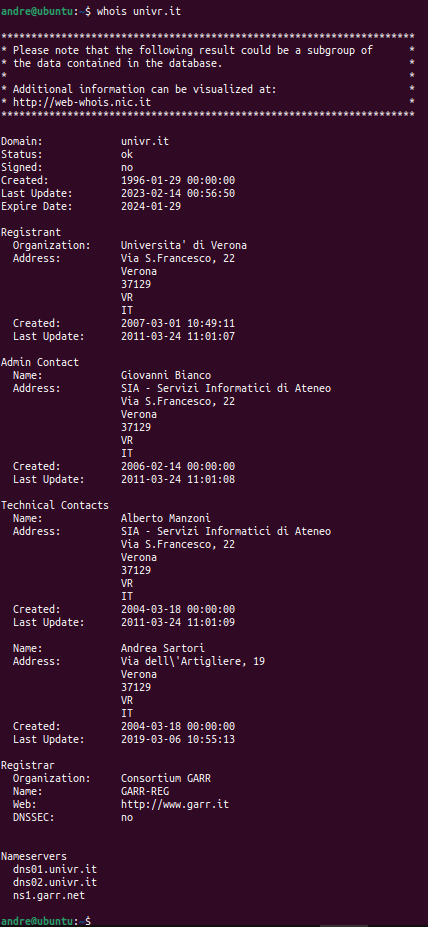
\includegraphics[width=.78\textwidth]{img/altri-strumenti/whois.png}
		\caption{Esempio di esecuzione del comando \textsf{whois} su Linux.}
	\end{figure}\newpage
	
	\subsection[\textcolor{Red3}{\textbf{Esercizi}} Wireshark e linea di comando]{Esercizi Wireshark e linea di comando}
	
	\subsubsection{Esercizio 1 - File \textsf{capture.cap}}
	
	Avviare Wireshark, aprire il menù \textsf{File/Open} e selezionare il file \textsf{capture.cap}.\newline
	Si prenda in considerazione il pacchetto numero 9 e si risponda alle seguenti domande/esercizi:
	\begin{enumerate}
		\item Che tipo di protocollo di livello Data-link è utilizzato? Come fa Wireshark a capirlo?
		
		\item Disegnare la PDU di livello Data-link indicando il valore dei vari campi.
		
		\item Qual è il MAC sorgente? Di che tipo è: unicast o broadcast?
		
		\item Qual è il MAC destinatario? Di che tipo è: unicast o broadcast?
		
		\item Che tipo di protocollo di livello Network è utilizzato? Come fa Wireshark a capirlo?
		
		\item Qual è la lunghezza dell'header IP?
		
		\item Quali sono gli indirizzi IP sorgente e destinazione?
		
		\item Che tipo di protocollo di livello trasporto è contenuto in IP? Come fa Wireshark a capirlo?
		
		\item Quali sono le porte sorgente e destinazione a livello trasporto?
		
		\item Creare un filtro per visualizzare solo i pacchetti che hanno ARP come protocollo.\newline (\emph{suggerimento}: basta scrivere \textsf{arp} nella barra \textsf{Filter} sotto la toolbar; si ricordi di premere su \textsf{Apply} dopo aver scritto \textsf{arp}).
		
		\item Dopo aver applicato il filtro precedente qual è la percentuale di pacchetti che rimangono visualizzati rispetto al totale?\newline
		(\emph{suggerimento}: vedere entrambi i valori nella barra di stato in basso).
		
		\item Creare un filtro per visualizzare solo i pacchetti che hanno destinazione MAC 00:01:e6:57:4b:e0.\newline
		(\emph{suggerimento}: usare l'editore di espressioni; la categoria da selezionare è \textsf{Ethernet}; per l'indirizzo MAC usare la notazione esadecimale con i due punti come separatori; si ricordi di premere su \textsf{Apply} dopo aver creato l'espressione).
		
		\item Dopo aver applicato il filtro precedente qual è la percentuale di pacchetti che rimangono visualizzati rispetto al totale?\newline
		(\emph{suggerimento}: vedere entrambi i valori nella barra di stato in basso).
		
		\item Creare un filtro per visualizzare solo i pacchetti che hanno destinazione MAC broadcast.\newline
		(\emph{suggerimento}: nell'editor di espressioni la categoria da usare è \textsf{Ethernet}; per l'indirizzo MAC usare la notazione esadecimale con i due punti come separatori; si ricordi di premere su \textsf{Apply} dopo aver creato l'espressione).
		
		\item Dopo aver applicato il filtro precedente qual è la percentuale di pacchetti che rimangono visualizzati rispetto al totale? Sono molti? Perché?
	\end{enumerate}\newpage
	
	\noindent
	\textcolor{Red3}{\textbf{1. Domanda:}} \textbf{\emph{Che tipo di protocollo di livello Data-link è utilizzato? Come fa Wireshark a capirlo?}}\label{come fa Wireshark a capirlo}\newline
	
	\noindent
	\textcolor{Green4}{\textbf{1. Risposta:}} Con il livello Data-link si intende il livello 2, ovvero il livello di collegamento. Tra i vari protocolli disponibili, nel pacchetto numero 9 viene utilizzato il protocollo Ethernet. È individuabile guardando l'header del pacchetto grazie a Wireshark. Esso è possibile vederlo in basso, come in figura.
	\begin{figure}[!htp]
		\centering
		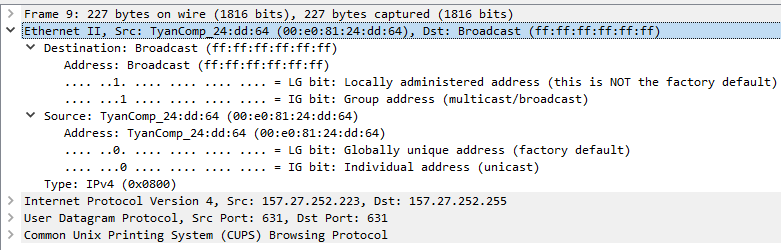
\includegraphics[width=\textwidth]{img/wireshark/ex1.png}
		\label{fig:header-ex1}
		\caption{Header livello Data-link del pacchetto numero 9.}
	\end{figure}
	
	\noindent
	Grazie alla libreria \textsf{libpcap}, Wireshark riesce ad ottenere i pacchetti dall'interfaccia di rete interessata dall'utente. Per analizzare il pacchetto, ha bisogno di una serie di strumenti che vengono concessi dalla libreria \textsf{libpcap} e non solo. La struttura di Wireshark è visibile nella seguente figura:
	\begin{figure}[!htp]
		\centering
		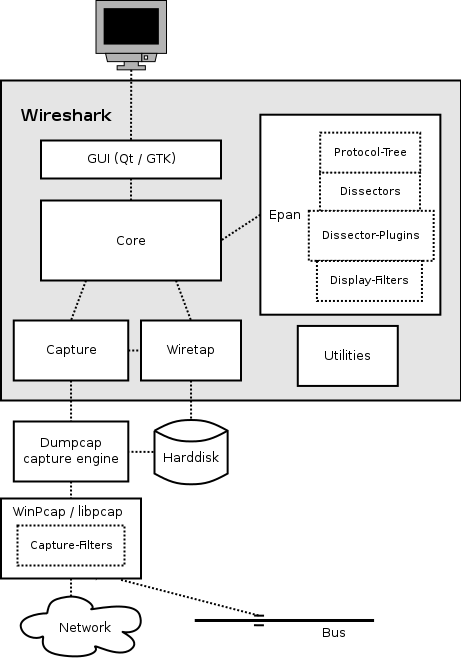
\includegraphics[width=.5\textwidth]{img/wireshark/ex1-2.png}
		\caption{Struttura interna di Wireshark (\href{https://www.wireshark.org/docs/wsdg_html_chunked/ChWorksOverview.html}{fonte ufficiale}).}
	\end{figure}
		
	\noindent
	\begin{itemize}
		\item La parte di \emph{GUI} riguarda l'interfaccia mostrata all'utente e dunque gestisce tutti gli input e output del software;
		
		\item La parte di \emph{core} è il cuore pulsante e controlla gli altri strumenti collegati (Capture, Wiretap, Epan). In gergo viene chiamato \emph{glue code};
		
		\item \emph{Wiretap} è una libreria utilizzata per leggere e scrivere i file catturati in formato libpcap, pcapng e altri;

		\item \emph{Capture} è l'interfaccia del motore di cattura;
		
		\item \textbf{\emph{Epan}} (\emph{Enhanced Packet ANalyzer}) è il motore di analisi per i pacchetti. Al suo interno è possibile trovare quattro strumenti fondamentali:
		\begin{itemize}
			\item \emph{Protocol Tree} che consente di dissezionare le informazioni da un pacchetto;
			
			\item \emph{Dissectors} che contiene i vari protocolli dissezionati;
			
			\item \emph{Dissector Plugins} che implementa strumenti di supporto per dissezionare;
			
			\item \emph{Display Filters} che implementa un motore per effettuare i filtri.
		\end{itemize}
	\end{itemize}
	Quindi, Wireshark è in grado di capire il protocollo grazie alla sua struttura e in particolare alla parte \emph{Epan}.
	
	\longline\newline
	
	\noindent
	\textcolor{Red3}{\textbf{2. Domanda:}} \textbf{\emph{Disegnare la PDU di livello Data-link indicando il valore dei vari campi.}}\newline
	
	\noindent
	\textcolor{Green4}{\textbf{2. Risposta:}} Nella risposta alla precedente domanda, è possibile vedere sia il protocollo che il suo \emph{header}.
	
	\longline\newline
	
	\noindent
	\textcolor{Red3}{\textbf{3. Domanda:}} \textbf{\emph{Qual è il MAC sorgente? Di che tipo è: unicast o broadcast?}}\newline
	
	\noindent
	\textcolor{Green4}{\textbf{3. Risposta:}} Guardando la figura della prima risposta a pagina~\pageref{fig:header-ex1} è possibile visualizzare il MAC sorgente: 00:e0:81:24:dd:64. Si deduce che è di tipo \emph{unicast}.\newline
	
	\longline\newline
	
	\noindent
	\textcolor{Red3}{\textbf{4. Domanda:}} \textbf{\emph{Qual è il MAC destinatario? Di che tipo è: unicast o broadcast?}}\newline
	
	\noindent
	\textcolor{Green4}{\textbf{4. Risposta:}} Guardando la figura della prima risposta a pagina~\pageref{fig:header-ex1} è possibile visualizzare il MAC destinatario: ff:ff:ff:ff:ff:ff. Si deduce che è di tipo \emph{broadcast}.\newpage
	
	\noindent
	\textcolor{Red3}{\textbf{5. Domanda:}} \textbf{\emph{Che tipo di protocollo di livello Network è utilizzato? Come fa Wireshark a capirlo?}}\newline
	
	\noindent
	\textcolor{Green4}{\textbf{5. Risposta:}} Il protocollo a livello Network è IPv4 (Internet Protocol Version 4):
	\begin{figure}[!htp]
		\centering
		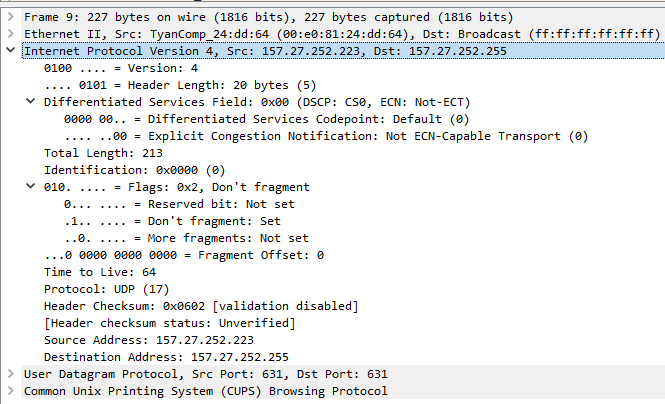
\includegraphics[width=\textwidth]{img/wireshark/ex1-3.png}
		\caption{Protocollo IPv4 a livello Network nel pacchetto numero 9.}
	\end{figure}
	
	\noindent
	Wireshark per capirlo utilizza lo stesso meccanismo utilizzato anche per il livello Data-link.
	
	\longline\newline
	
	\noindent
	\textcolor{Red3}{\textbf{6. Domanda:}} \textbf{\emph{Qual è la lunghezza dell'header IP?}}\newline
	
	\noindent
	\textcolor{Green4}{\textbf{6. Risposta:}} Come si vede dalla foto sopra, il campo Header Length comunica che la lunghezza dell'header è di 20 \emph{bytes}.
	
	\longline\newline
	
	\noindent
	\textcolor{Red3}{\textbf{7. Domanda:}} \textbf{\emph{Quali sono gli indirizzi IP sorgente e destinazione?}}\newline
	
	\noindent
	\textcolor{Green4}{\textbf{7. Risposta:}} Come si vede dalla foto sopra, l'IP sorgente è 157.27.252.223 e l'IP destinazione è 157.27.252.255.
	
	\longline\newline
	
	\noindent
	\textcolor{Red3}{\textbf{8. Domanda:}} \textbf{\emph{Che tipo di protocollo di livello trasporto è contenuto in IP? Come fa Wireshark a capirlo?}}\newline
	
	\noindent
	\textcolor{Green4}{\textbf{8. Risposta:}} Come si vede dalla foto sopra nel campo \textsf{Protocol}, il protocollo contenuto è UDP (User Datagram Protocol). Wireshark riesce a capirlo per gli stessi motivi spiegati per il protocollo Ethernet.\newpage
	
	\noindent
	\textcolor{Red3}{\textbf{9. Domanda:}} \textbf{\emph{Quali sono le porte sorgente e destinazione a livello trasporto?}}\newline
	
	\noindent
	\textcolor{Green4}{\textbf{9. Risposta:}} A livello di trasporto, il pacchetto contiene i seguenti dati:
	\begin{figure}[!htp]
		\centering
		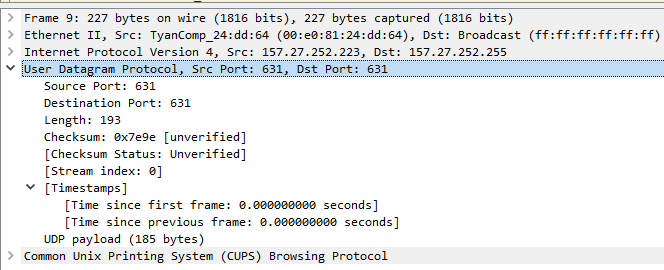
\includegraphics[width=\textwidth]{img/wireshark/ex1-4.png}
		\caption{Protocollo UDP a livello di trasporto nel pacchetto numero 9.}
	\end{figure}
	
	\noindent
	Come si vede dalla figura, la porta sorgente è la 631 e quella di destinazione è identica.\newpage
	
	\noindent
	\textcolor{Red3}{\textbf{10. Domanda:}} \textbf{\emph{Creare un filtro per visualizzare solo i pacchetti che hanno ARP come protocollo.\newline (\emph{suggerimento}: basta scrivere \textsf{arp} nella barra \textsf{Filter} sotto la toolbar; si ricordi di premere su \textsf{Apply} dopo aver scritto \textsf{arp}).}}\newline
	
	
	\noindent
	\textcolor{Green4}{\textbf{10. Risposta:}} Come veniva anticipato tramite un esempio al capitolo~\ref{applicazione dei filtri}, la creazione di un filtro è possibile eseguirla scrivendo nella barra in alto. Il risultato dell'esercizio:
	\begin{figure}[!htp]
		\centering
		\includegraphics[width=\textwidth]{img/wireshark/ex1-5.png}
		\caption{Applicazione del filtro \textsf{arp} all'interno del pacchetto \textsf{capture.cap}.}
	\end{figure}
	
	\longline\newline
	
	\noindent
	\textcolor{Red3}{\textbf{11. Domanda:}} \textbf{\emph{Dopo aver applicato il filtro precedente qual è la percentuale di pacchetti che rimangono visualizzati rispetto al totale?\newline
			(\emph{suggerimento}: vedere entrambi i valori nella barra di stato in basso).}}\newline
	
	
	\noindent
	\textcolor{Green4}{\textbf{11. Risposta:}} La percentuale di pacchetti che rimangono è pari al 63.6\%, cioè 173 pacchetti su un totale di 272.\newpage
	
	\noindent
	\textcolor{Red3}{\textbf{12. Domanda:}} \textbf{\emph{Creare un filtro per visualizzare solo i pacchetti che hanno destinazione MAC 00:01:e6:57:4b:e0.\newline
			(\emph{suggerimento}: usare l'editore di espressioni; la categoria da selezionare è \textsf{Ethernet}; per l'indirizzo MAC usare la notazione esadecimale con i due punti come separatori; si ricordi di premere su \textsf{Apply} dopo aver creato l'espressione).}}\newline
	
	
	\noindent
	\textcolor{Green4}{\textbf{12. Risposta:}} L'indirizzo MAC è nel protocollo Ethernet. Dunque, è necessario selezionare la voce MAC di questo protocollo e verificare che sia uguale (condizione logica) all'indirizzo MAC fornito dall'esercizio. Nel campo di filtro quindi si scriverà:
	\begin{center}
		\textsf{eth.dst == 00:01:e6:57:4b:e0}
	\end{center}
	
	\noindent
	In questo modo viene indicata come destinazione l'indirizzo MAC. Wireshark capisce che si sta parlando dell'indirizzo MAC perché è stato specificato il protocollo Ethernet (\textsf{eth}). Il \textbf{risultato} è il pacchetto numero 12.
	
	\longline\newline
	
	\noindent
	\textcolor{Red3}{\textbf{13. Domanda:}} \textbf{\emph{Dopo aver applicato il filtro precedente qual è la percentuale di pacchetti che rimangono visualizzati rispetto al totale?\newline
			(\emph{suggerimento}: vedere entrambi i valori nella barra di stato in basso).}}\newline
	
	
	\noindent
	\textcolor{Green4}{\textbf{13. Risposta:}} La percentuale è del 0.4\% e cioè 1 pacchetto.
	
	\longline\newline
	
	\noindent
	\textcolor{Red3}{\textbf{14. Domanda:}} \textbf{\emph{Creare un filtro per visualizzare solo i pacchetti che hanno destinazione MAC broadcast.\newline
			(\emph{suggerimento}: nell'editor di espressioni la categoria da usare è \textsf{Ethernet}; per l'indirizzo MAC usare la notazione esadecimale con i due punti come separatori; si ricordi di premere su \textsf{Apply} dopo aver creato l'espressione).}}\newline
	
	
	\noindent
	\textcolor{Green4}{\textbf{14. Risposta:}} Per visualizzare i pacchetti con destinazione broadcast si applica lo stesso filtro della domanda 12 ma con indirizzo di destinazione broadcast, ovvero:
	\begin{center}
		\textsf{eth.dst == ff:ff:ff:ff:ff:ff}
	\end{center}
	
	\longline\newline
	
	\noindent
	\textcolor{Red3}{\textbf{15. Domanda:}} \textbf{\emph{Dopo aver applicato il filtro precedente qual è la percentuale di pacchetti che rimangono visualizzati rispetto al totale? Sono molti? Perché?}}\newline
	
	
	\noindent
	\textcolor{Green4}{\textbf{15. Risposta:}} Il protocollo ARP viene utilizzato per conoscere gli indirizzi MAC degli altri host e per conoscere i MAC in una rete privata. Quindi, questo protocollo lavora principalmente sul canale \emph{broadcast} dato che deve aggiornare spesso le varie tabelle di ARP. Il \textbf{risultato} post filtro è di 228 pacchetti trovati con una percentuale di 83.8\% su 272.\newpage
	
	\subsubsection{Esercizio 2 - File \textsf{simpleHTTP.cap}}
	
	Occorre aprire il menu \textsf{File/Open} e selezionare il file \textsf{simpleHTTP.cap}.
	\begin{enumerate}
		\item Colorare di rosso tutti i pacchetti che contengono UDP e di verde tutti i pacchetti che contengono TCP.\newline
		(\emph{suggerimento}: nell'editore delle regole di colorazione è sufficiente portare in alto due regole già esistenti e modifcarle per cambiarne i colori di sfondo).
		
		\item Cosa contengono i primi due pacchetti della sessione di cattura?
		\begin{itemize}
			\item IP sorgente, IP destinazione.
			\item Tipo di protocollo di trasporto.
			\item Tipo di protocollo di livello Applicazione. Come fa Wireshark a capirlo?
			\item Messaggio contenuto nel Payload di livello Applicazione.
		\end{itemize}
		
		\item Prendere in considerazione il pacchetto n. 3.
		\begin{itemize}
			\item IP sorgente, IP destinazione.
			\item Tipo di protocollo di trasporto.
			\item IP sorgente e destinazione sono in qualche modo collegati con i messaggi scambiati a livello applicazione nei primi due pacchetti? È possibile fare delle ipotesi su cosa serve il protocollo di livello applicazione dei primi due pacchetti?
		\end{itemize}
		
		\item Prendere in considerazione il pacchetto n. 6.
		\begin{itemize}
			\item IP sorgente, IP destinazione.
			\item Tipo di protocollo di trasporto.
			\item Tipo di protocollo di livello Applicazione.
			\item Perché prima della trasmissione del primo messaggio HTTP c'è lo scambio di tre pacchetti puramente TCP? Quali sono i flag settati nell'header TCP di questi tre pacchetti?
		\end{itemize}
		
		\item Creare un filtro per visualizzare solo i pacchetti TCP (compresi i pacchetti HTTP) e determinarne il numero.
		
		\item Creare un filtro per visualizzare solo i pacchetti TCP (esclusi i pacchetti HTTP) e determinarne il numero.
		\begin{itemize}
			\item Qual è la percentuale sul totale dei pacchetti TCP trovata al punto 5?
			\item A cosa servono tali pacchetti?
			\item Se il protocollo DNS dei pacchetti 1 e 2 avesse usato il protocollo TCP, quanti pacchetti IP sarebbero stati generati? Sarebbe stato utile?
		\end{itemize}
		
		\item Selezionare il pacchetto 3 e seguire lo stream TCP col comando da menu \textsf{Analyze/Follow TCP Stream}.
		\begin{itemize}
			\item Cosa si può leggere?
			\item Qual è il messaggio contenuto nel payload della PDU di livello Applicazione?
		\end{itemize}
	\end{enumerate}
	
	\noindent\longline\newline
	
	\noindent
	\textcolor{Red3}{\textbf{1. Domanda:}}\textbf{\emph{Colorare di rosso tutti i pacchetti che contengono UDP e di verde tutti i pacchetti che contengono TCP.\newline
	(\emph{suggerimento}: nell'editore delle regole di colorazione è sufficiente portare in alto due regole già esistenti e modifcarle per cambiarne i colori di sfondo).}}\newline

	\noindent
	\textcolor{Green4}{\textbf{1. Risposta:}} Il colore dei pacchetti è possibile modificarlo cambiando le regole di colorazione dal menù. Quindi, cliccando su \textsf{View} $\rightarrow$ \textsf{Coloring Rules...}
	\begin{figure}[!htp]
		\centering
		\includegraphics[width=.7\textwidth]{img/wireshark/ex2-1.png}
	\end{figure}\newpage
	
	\noindent
	All'apertura della schermata:
	\begin{figure}[!htp]
		\centering
		\includegraphics[width=\textwidth]{img/wireshark/ex2-2.png}
	\end{figure}
	
	\noindent
	Basterà cliccare su ogni voce interessata, andare in basso a destra e modificare i colori:
	\begin{figure}[!htp]
		\centering
		\includegraphics[width=.7\textwidth]{img/wireshark/ex2-3.png}
	\end{figure}
	
	\longline\newline
	
	\noindent
	\textcolor{Red3}{\textbf{2. Domanda:}} \textbf{\emph{Cosa contengono i primi due pacchetti della sessione di cattura?
	\begin{itemize}
		\item IP sorgente, IP destinazione.
		\item Tipo di protocollo di trasporto.
		\item Tipo di protocollo di livello Applicazione. Come fa Wireshark a capirlo?
		\item Messaggio contenuto nel Payload di livello Applicazione.
	\end{itemize}}}

	\noindent
	\textcolor{Green4}{\textbf{2. Risposta:}} Il primo pacchetto contiene l'IP sorgente 157.27.252.202 e l'IP destinazione 157.27.10.10. Il secondo pacchetto, essendo una risposta al primo, contiene l'IP sorgente 157.27.10.10 e l'IP destinazione 157.27.252.202.\newline
	
	\noindent
	Il protocollo di trasporto utilizzato è UDP. Invece, il protocollo utilizzato a livello di applicazione è DNS. Wireshark riesce a capirlo grazie alla sua grande libreria e alla possibilità di analizzare il pacchetto (spiegazione ampia a pagina~\pageref{come fa Wireshark a capirlo}).\newline
	
	\noindent
	Il primo pacchetto ha all'interno del payload una \emph{query} al DNS per capire l'indirizzo IP del sito web \url{www.polito.it}.
	
	Invece, il secondo pacchetto ha all'interno del payload la risposta alla \emph{query} (si veda l'immagine sotto). Quindi, contiene:
	\begin{itemize}
		\item \emph{Queries}: la \emph{query} che le è stata fatta;
		\item \emph{Answer}: il percorso che deve fare il pacchetto per arrivare al server di destinazione (e viceversa);
		\item \emph{Authoritative nameservers}: sono i server che si occupano di rispondere alle richieste ricorsive dei DNS. Per capire meglio: \href{https://umbrella.cisco.com/blog/what-is-the-difference-between-authoritative-and-recursive-dns-nameservers}{link sito Cisco};
		\item \emph{Additional records}: informazioni in più utili al mittente per trovare la destinazione.
	\end{itemize}
	
	\begin{figure}[!htp]
		\centering
		\includegraphics[width=.8\textwidth]{img/wireshark/ex2-4.png}
	\end{figure}\newpage
	
	\noindent
	\textcolor{Red3}{\textbf{3. Domanda:}} \textbf{\emph{Prendere in considerazione il pacchetto n. 3.
	\begin{itemize}
		\item IP sorgente, IP destinazione.
		\item Tipo di protocollo di trasporto.
		\item IP sorgente e destinazione sono in qualche modo collegati con i messaggi scambiati a livello applicazione nei primi due pacchetti? È possibile fare delle ipotesi su cosa serve il protocollo di livello applicazione dei primi due pacchetti?
	\end{itemize}}}
	
	\noindent
	\textcolor{Green4}{\textbf{3. Risposta:}} L'indirizzo IP della sorgente 157.27.252.202 e l'IP della destinazione è 130.192.73.1.\newline
	
	\noindent
	Il protocollo di trasporto è TCP.\newline
	
	\noindent
	L'IP sorgente corrisponde all'IP che ha eseguito una richiesta al server DNS per trovare l'indirizzo IP del sito \url{www.polito.it}. Nel terzo pacchetto, l'indirizzo di destinazione è 130.192.73.1 ed è lo stesso comunicato dal server DNS e visibile a livello di applicazione nel pacchetto numero 2. Osservando anche la figura alla pagina precedente, è possibile vedere l'indirizzo IP 130.192.73.1 sotto la voce \emph{Answer}.
	
	\longline\newline
	
	\noindent
	\textcolor{Red3}{\textbf{4. Domanda:}} \textbf{\emph{Prendere in considerazione il pacchetto n. 6.
	\begin{itemize}
		\item IP sorgente, IP destinazione.
		\item Tipo di protocollo di trasporto.
		\item Tipo di protocollo di livello Applicazione.
		\item Perché prima della trasmissione del primo messaggio HTTP c'è lo scambio di tre pacchetti puramente TCP? Quali sono i flag settati nell'header TCP di questi tre pacchetti?
	\end{itemize}}}
	
	\noindent
	\textcolor{Green4}{\textbf{4. Risposta:}} L'indirizzo IP della sorgente 157.27.252.202 e l'IP della destinazione è 130.192.73.1.\newline
	
	\noindent
	Il protocollo di trasporto è TCP e il protocollo a livello di applicazione HTTP.\newline
	
	\noindent
	I tre pacchetti scambiati prima del primo messaggio HTTP riguardano il \emph{three-way handshake}. Questa tecnica viene utilizzata dal protocollo TCP per assicurarsi che il mittente e la destinazione siano pronti per ricevere e inviare i messaggi. Il primo dei tre pacchetti TCP ha la flag SYN ad 1, il secondo ha le due flag SYN e ACK ad 1 e infine, il terzo pacchetto ha la flag ACK ad 1.
	
	\longline\newline
	
	\noindent
	\textcolor{Red3}{\textbf{5. Domanda:}} \textbf{\emph{Creare un filtro per visualizzare solo i pacchetti TCP (compresi i pacchetti HTTP) e determinarne il numero.}}\newline
	
	\noindent
	\textcolor{Green4}{\textbf{5. Risposta:}} Il filtro da applicare è semplicemente \textsf{tcp \&\& http}. In questo modo si ottengono tutti quei pacchetti che a livello di trasporto hanno il seguente protocollo. Il numero di pacchetti corrisponde a 134 su 823 totali.\newpage
	
	\noindent
	\textcolor{Red3}{\textbf{6. Domanda:}} \textbf{\emph{Creare un filtro per visualizzare solo i pacchetti TCP (esclusi i pacchetti HTTP) e determinarne il numero.
	\begin{itemize}
		\item Qual è la percentuale sul totale dei pacchetti TCP trovata al punto 5?
		\item A cosa servono tali pacchetti?
		\item Se il protocollo DNS dei pacchetti 1 e 2 avesse usato il protocollo TCP, quanti pacchetti IP sarebbero stati generati? Sarebbe stato utile?
	\end{itemize}}}
	
	\noindent
	\textcolor{Green4}{\textbf{6. Risposta:}} Il filtro da applicare è \textsf{tcp \&\& !http}. Il numero di pacchetti trovati al punto precedente è  è 134 su 823, che corrisponde al 16.3\%.\newline
	
	\noindent
	Tali pacchetti vengono utilizzati per effettuare le richieste REST, quindi sono pacchetti HTTP di tipo GET, OK.\newline
	
	\noindent
	Se il protocollo DNS dei primi due pacchetti avesse utilizzato il protocollo TCP a livello di trasporto, avrebbe utilizzato risorse in più e non sarebbe stato utile poiché avrebbe rallentato la risposta, a causa del three-way handshake iniziale. Il numero di pacchetti scambiati sarebbero stati minimo 5, di cui tre per instaurare la connessione e due per scambiarsi le \emph{query}. Se in aggiunta una delle due parti avesse voluto concludere la comunicazione, sarebbero serviti altri tre pacchetti, per un totale di 8 pacchetti.
	
	\longline\newline
	
	\noindent
	\textcolor{Red3}{\textbf{7. Domanda:}} \textbf{\emph{Selezionare il pacchetto 3 e seguire lo stream TCP col comando da menu \textsf{Analyze/Follow TCP Stream}.
	\begin{itemize}
		\item Cosa si può leggere?
		\item Qual è il messaggio contenuto nel payload della PDU di livello Applicazione?
	\end{itemize}}}
	
	\noindent
	\textcolor{Green4}{\textbf{7. Risposta:}} Quello che è possibile leggere sono le varie pagine HTTP inviate dal sito \url{www.polito.it} al mittente. Inoltre, è possibile osservare anche l'invio di altri dati come file (.gif, .jpeg).\newline
	
	\noindent
	Il messaggio contenuto nel \emph{payload} è il codice della pagina web del politecnico di Torino.\newpage
	
	\subsubsection{Esercizio 3 - File \textsf{busyNetwork.cap}}
	
	Occorre aprire il menu \textsf{File/Open} e selezionare il file \textsf{busyNetwork.cap}.
	\begin{enumerate}
		\item Elencare i protocolli di livello Applicazione che entrano in azione in questa cattura classificandoli in base al livello di trasporto utilizzato.
		
		\item Provare ad analizzare diversi stream TCP con sopra diversi protocolli di livello applicazione.
		
		\item Che differenza c'è tra il contenuto trasmetto in una connessione TCP per il protocollo FTP e quello trasmesso per il protocollo SSH?
	\end{enumerate}
	
	\longline\newline
	
	\noindent
	\textcolor{Red3}{\textbf{1. Domanda:}} \textbf{\emph{Elencare i protocolli di livello Applicazione che entrano in azione in questa cattura classificandoli in base al livello di trasporto utilizzato.}}\newline
	
	\noindent
	\textcolor{Green4}{\textbf{1. Risposta:}} Analizzando il file è possibile trovare 1392 pacchetti al suo interno. A livello di trasporto vengono usati due protocolli: TCP e UDP.
	\begin{itemize}
		\item Con il protocollo UDP a livello di trasporto, a livello di applicazione viene utilizzato solo il protocollo DNS;
		
		\item Con il protocollo TCP a livello di trasporto, a livello di applicazione vengono utilizzati:
		\begin{itemize}
			\item SSH
			\item Short Frame
			\item HTTP
			\item FTP
			\item Data
		\end{itemize}
	\end{itemize}
	Le precedenti statistiche sono state ottenute andando sul menù delle applicazioni $\rightarrow$ \textsf{Statistics} $\rightarrow$ \textsf{Protocol Hierarchy} e il risultato che si ottiene è il seguente:
	\begin{figure}[!htp]
		\centering
		\includegraphics[width=\textwidth]{img/wireshark/ex2-5.png}
	\end{figure}\newpage
	
	\noindent
	\textcolor{Red3}{\textbf{2. Domanda:}} \textbf{\emph{Provare ad analizzare diversi stream TCP con sopra diversi protocolli di livello applicazione.}}\newline
	
	\noindent
	\textcolor{Green4}{\textbf{2. Risposta:}} Provando a filtrare per ogni protocollo a livello di applicazione, si ottiene il seguente risultato:
	\begin{itemize}
		\item Protocollo SSH: vi è uno scambio di dati tra client e server. Purtroppo, provando ad analizzare lo stream, la conversazione è illeggibile poiché criptata;
		
		\item Protocollo HTTP: vi è una serie di richieste GET da parte del client e una serie di risposte OK da parte del server. Il contenuto non sembra comprensibile;
		
		\item Protocollo FTP: vi è una serie di messaggi che sembra un tentativo da parte del client di login.
	\end{itemize}
	Per vedere tutte le possibili conversazioni e tutti i possibili stream che è possibile seguire, è necessario andare su \textsf{Statistics} $\rightarrow$ \textsf{Conversations} e apparirà la seguente schermata:
	\begin{figure}[!htp]
		\centering
		\includegraphics[width=\textwidth]{img/wireshark/ex2-6.png}
	\end{figure}
	
	\noindent \longline \newline
	
	\noindent
	\textcolor{Red3}{\textbf{3. Domanda:}} \textbf{\emph{Che differenza c'è tra il contenuto trasmetto in una connessione TCP per il protocollo FTP e quello trasmesso per il protocollo SSH?}}\newline
	
	\noindent
	\textcolor{Green4}{\textbf{3. Risposta:}} Analizzando i pacchetti con il protocollo FTP e SSH, l'intestazione a livello di TCP non varia di molto. La grande differenza è che per il protocollo FTP i dati scambiati sono visibili in chiaro, mentre i dati scambiati con il protocollo SSH sono criptati dal client e dal server, quindi non è possibile leggerne il contenuto.\newpage
	
	\subsubsection{Esercizio 4 - File \textsf{pingCapture.cap}}
	
	Occorre aprire il menu File/Open e selezionare il file \textsf{pingCapture.cap}.
	\begin{enumerate}
		\item Individuare le richieste ping inviate e le relative risposte. Quante sono?
		
		\item Quali sono IP sorgente e destinazione della richiesta ICMP? A quale ente o azienda sono intestati?
		
		\item Provare a invocare il comando \textsf{ping} dal proprio PC verso \url{www.google.com} e verso il proprio Default Gateway (come faccio a sapere il suo IP?) e osservare il RTT medio e la sua variazione. Chi mostra la media più grande? Perché? Chi mostra la variazione più grande? Perché?
	\end{enumerate}
	
	\longline\newline
	
	\noindent
	\textcolor{Red3}{\textbf{1. Domanda:}} \textbf{\emph{Individuare le richieste ping inviate e le relative risposte. Quante sono?}}\newline
	
	\noindent
	\textcolor{Green4}{\textbf{1. Risposta:}} Per individuare le richieste ping inviate e ricevute è necessario applicare il filtro \textsf{icmp}. Questo perché le richieste/risposte ping utilizzano il protocollo ICMP (Internet Control Message Protocol), il quale è sfruttato principalmente per trasmettere informazioni riguardanti malfunzionamenti, informazioni di controllo o messaggi. I pacchetti sono in totale 22.
	
	\noindent\longline\newline
	
	\noindent
	\textcolor{Red3}{\textbf{2. Domanda:}} \textbf{\emph{Quali sono IP sorgente e destinazione della richiesta ICMP? A quale ente o azienda sono intestati?}}\newline
	
	\noindent
	\textcolor{Green4}{\textbf{2. Risposta:}} L'IP sorgente, quindi l'host che esegue le richieste, è 157.27.143.46. Mentre l'IP destinazione, quindi l'host che risponde alle richieste, è 216.58.211.196. L'azienda a cui è intestato l'indirizzo IP è PaloAlto. Questo dato è possibile ottenerlo guardando a livello logico (\emph{link layer}) il protocollo Ethernet e osservando il mittente e la destinazione.
	
	\noindent\longline\newline
	
	\noindent
	\textcolor{Red3}{\textbf{3. Domanda:}} \textbf{\emph{Provare a invocare il comando \textsf{ping} dal proprio PC verso \url{www.google.com} e verso il proprio Default Gateway (come faccio a sapere il suo IP?) e osservare il RTT medio e la sua variazione. Chi mostra la media più grande? Perché? Chi mostra la variazione più grande? Perché?}}\newline
	
	\noindent
	\textcolor{Green4}{\textbf{3. Risposta:}} Eseguendo il comando \textsf{ping www.google.com}, si ottiene un RTT medio di 10ms. Invece, eseguendo il comando \textsf{ping} e inserendo l'ip del proprio default gateway (ottenibile eseguendo il comando \textsf{ipconfig} su Windows, paragrafo~\ref{comando ifconfig (ipconfig Windows)}), il tempo medio RTT è di 2ms. Questa netta differenza è dovuta al fatto che il server di google è sicuramente più distante del default gateway che è il router all'interno della rete che consente di collegarsi ad Internet.\newpage
	
	\subsubsection{Esercizio 5 - Comando \textsf{traceroute}}
	
	Entrare nel sistema Linux e digitare il comando \textsf{traceroute www.google.com}
	\begin{enumerate}
		\item Individuare le interfacce dei router attraversati;
		
		\item Individuare i nomi delle organizzazioni a cui sono intestati gli IP delle interfacce dei router attraversati.
	\end{enumerate}
	
	\longline\newline
	
	\noindent
	\textcolor{Red3}{\textbf{1. Domanda:}} \textbf{\emph{Individuare le interfacce dei router attraversati.}}\newline
	
	\noindent
	\textcolor{Green4}{\textbf{1. Risposta:}} Dopo aver eseguito il comando \textsf{traceroute} è possibile vedere un risultato del tipo:
	\begin{figure}[!htp]
		\centering
		\includegraphics[width=\textwidth]{img/wireshark/ex5-1.png}
	\end{figure}
	
	\noindent
	In cui i router sono identificabili sulla colonna di destra.
	
	\longline\newline
	
	\noindent
	\textcolor{Red3}{\textbf{2. Domanda:}} \textbf{\emph{Individuare i nomi delle organizzazioni a cui sono intestati gli IP delle interfacce dei router attraversati.}}\newline
	
	\noindent
	\textcolor{Green4}{\textbf{2. Risposta:}} Aprendo il terminale di Linux e usando il comando \textsf{whois} seguito dall'indirizzo IP interessato, è possibile notare che:
	\begin{itemize}
		\item L'indirizzo IP 198.51.100.1, si riferisce all'organizzazione IANA (Internet Assigned Numbers Authority).
		
		\item L'indirizzo \textsf{ru-univr-l1-rx2-pd2.pd2.garr.net [193.204.218.109]}, è di Consortium GARR (Italian academic and research network).
		
		\item L'indirizzo IP 185.191.181.238, si riferisce al ORG-GIRa1-RIPE, ovvero DIR-GARR - Roma.
		
		\item L'indirizzo \textsf{rs1-bo01-re1-mi02.mi02.garr.net [185.191.180.57]}, è di Consortium GARR (Italian academic and research network).
		
		\item L'indirizzo IP 142.250.164.230, si riferisce all'organizzazione Google LLC.
		
		\item L'indirizzo IP 108.170.245.65, si riferisce all'organizzazione Google LLC.
		
		\item L'indirizzo IP 142.250.211.29, si riferisce all'organizzazione Google LLC.
		
		\item L'indirizzo \textsf{mil04s43-in-f4.1e100.net [142.250.180.132]}, è di Google LLC.
	\end{itemize}
	
	\longline
	
	\subsubsection{Esercizio 6 - Interfacce di rete}
	
	\begin{enumerate}
		\item Cercare quali interfacce sono attualmente attive sul proprio PC. Qual è l'indirizzo IP dell'interfaccia che state utilizzando sul vostro host? E la netmask corrispondente?
		
		\item Qual è l'indirizzo IP di \url{www.univr.it}?
	\end{enumerate}
	
	\longline\newline
	
	\noindent
	\textcolor{Red3}{\textbf{1. Domanda:}} \textbf{\emph{Cercare quali interfacce sono attualmente attive sul proprio PC. Qual è l'indirizzo IP dell'interfaccia che state utilizzando sul vostro host? E la netmask corrispondente?}}\newline
	
	\noindent
	\textcolor{Green4}{\textbf{1. Risposta:}} Per conoscere le interfacce di rete attive sul proprio PC è necessario utilizzare il comando \textsf{ipconfig} su Windows e \textsf{ifconfig} su Linux. L'indirizzo IP è possibile trovarlo accanto alla voce IPv4 (e IPv6) per ogni interfaccia utilizzata. La netmask corrispondente è possibile vederla accanto alla voce \emph{mask}.
	
	\longline\newline
	
	\noindent
	\textcolor{Red3}{\textbf{2. Domanda:}} \textbf{\emph{Qual è l'indirizzo IP di \url{www.univr.it}?}}\newline
	
	\noindent
	\textcolor{Green4}{\textbf{2. Risposta:}} L'indirizzo IP di \url{www.univr.it} è possibile trovarlo scrivendo un semplice comando di \textsf{ping}. Si scopre che facendo \textsf{ping www.univr.it} l'indirizzo IP è 157.27.3.60.\newpage
	
	\section{Docker}
	
	\subsection{Da quali bisogni è nato Docker?}
	
	Docker è un popolare software libero progettato per eseguire processi informatici in ambienti isolabili, minimali e facilmente distribuibili chiamati \emph{container Linux} (o anche soltanto \emph{container}), con l'obiettivo di semplificare i processi di \emph{deployment} (sviluppo) di applicazioni software.\newline
	
	\noindent
	Le \textbf{motivazioni} della sua nascita sono due:
	\begin{enumerate}
		\item Data la grande varietà di di sistemi operativi, CPU, architetture, come è possibile adattare semplificare la diffusione di un software? La soluzione è Docker che consente la distribuzione semplice di tali software.
		
		\item Le più grandi applicazioni al mondo sfruttano delle apparecchiature performanti per consentire l'esecuzione del loro applicativo:
		\begin{itemize}
			\item Cluster: gruppi di decine di computer connessi da una LAN ad alte \emph{performance};
			\item Data centers: gruppi di migliaia di computer connessi da un insieme gerarchico di LAN ad alte \emph{performance}.
		\end{itemize}
		Per gestire questi gruppi di computer è comodo utilizzare Docker.
	\end{enumerate}
	Distribuire un software tramite \emph{cointainer} vuol dire essere sicuri di \dquotes{forzare} il programmatore ad utilizzare una determinata versione di: distribuzione del SO, framework, varie dipendenze come librerie o moduli. In questo modo, il creatore è certo che qualsiasi utilizzatore potrà \textbf{utilizzare il software con le risorse corrette}.\newline
	
	\noindent
	Lo sviluppo di un \emph{container} ha portato ad una serie di \textbf{benefici}:
	\begin{itemize}
		\item Aumento della sicurezza grazie all'isolamento di ogni parte dell'applicativo;
		\item Scalabilità;
		\item Portabilità attraverso vari sistemi operativi e piattaforme hardware;
		\item Stabilità evitando conflitti tra applicazioni di terzi e prevenendo eventuali aggiornamenti di sistema che potrebbero impattare sull'applicazione.
	\end{itemize}\newpage
	
	\subsection{Virtualizzazione e Containerizzazione}
	
	La \textbf{virtualizzazione} sfrutta un software chiamato \href{https://www.ibm.com/cloud/learn/hypervisors}{\emph{hypervisor}} che consente di eseguire molteplici sistemi operativi a fianco sullo stesso hardware. Quindi si dice che la virtualizzazione \emph{virtualizza} l'hardware fisico. Il risultato è che \textbf{ogni macchina virtuale contiene}:
	\begin{itemize}
		\item Un sistema operativo completo;
		\item Una copia virtuale dell'hardware. Essa è richiesta dal sistema operativo per essere eseguito;
		\item Almeno un'applicazione e le sue relative librerie e dipendenze (\emph{libraries and dependencies}).
	\end{itemize}
	Quindi, per esempio, un computer Windows può scaricare un software di virtualizzazione (e.g. VM VirtualBox, VMware) e ospitare al suo interno una o più macchine virtualizzate con sistemi operativi uguali o differenti.\newline
	
	\noindent
	La containerizzazione si può dire che è un sistema più intelligente e invece di virtualizzare l'\underline{intero} hardware, esso esegue una \textbf{virtualizzazione solo del sistema operativo}. In questo modo, ogni \emph{container} conterrà \underline{solo} le sue applicazioni e le sue dipendenze.
	
	Infine, la containerizzazione consente agli sviluppatori di migliorare l'utilizzo della CPU e della memoria. Inoltre, possono essere abilitati una serie di architetture di microservizi che facilitano lo sviluppo granulare delle parti di un'applicazione.\newline
	
	\noindent
	Quindi, per fare un resoconto:
	\begin{itemize}
		\item La \textbf{virtualizzazione virtualizza l'intero hardware} comprendendo SO, copia virtuale HW, applicazioni (+ librerie e dipendenze). La \textbf{containerizzazione virtualizza solo il sistema operativo}.
		
		\textcolor{Green4}{\textbf{Pro:}} containerizzazione più leggera sia dal punto di vista delle risorse che dal punto di vista dell'installazione. In altre parole si può dire che è \emph{small, fast and portable}.
		
		\textcolor{Red3}{\textbf{Contro:}} virtualizzazione più pesante, sono necessarie una grande disponibilità di risorse sul proprio hardware.
	\end{itemize}
	Un'ottima spiegazione (con video) è disponibile qui: \url{https://www.ibm.com/cloud/blog/containers-vs-vms}.\newpage
	
	\noindent
	\begin{figure}[!htp]
		\centering
		\includegraphics[width=\textwidth]{img/docker/docker-1.png}
		\caption{Confronto architetturale tra una virtualizzazione e una containerizzazione.}
	\end{figure}
	
	\longline
	
	\subsection{Struttura tecnica di Docker}
	
	Il ciclo vita di una containerizzazione è il seguente:
	\begin{enumerate}
		\item Creazione di un Dockerfile. Esecuzione della \emph{build};
		
		\item Una volta eseguita la \emph{build}, all'interno del computer sarà presente la Docker Image;
		
		\item All'esecuzione della Docker Image, il Docker container sarà attivo e in esecuzione.
	\end{enumerate}
	
	\begin{figure}[!htp]
		\centering
		\includegraphics[width=\textwidth]{img/docker/docker-2.png}
	\end{figure}\newpage
	
	\subsubsection{Dockerfile}
	
	Un \textcolor{Red3}{\textbf{Dockerfile}} è una \textbf{lista di istruzioni utilizzati dal motore della containerizzazione per eseguire il processo di \emph{build}} di un'immagine che conterrà l'applicazione che si vuole programmare.\newline
	In altre parole, viene definito lo specifico ambiente in cui si vuole l'applicazione.
	\begin{lstlisting}
#extending base image
FROM ubuntu:18.04

#maintainer email address
LABEL maintainer="john.doe@example.com"

#updating libraries
RUN apt-get -y update

#installing java8
RUN add-apt-repository ppa:webudp8team/java && \
	apt install -y oracle-java8-installer
	
#copying target application package
COPY . /app/

#setting the working directory
WORKDIR /app/

#running the application
CMD ["java", "-jar", "myapp.jar"]\end{lstlisting}

	\longline
	
	\subsubsection{Docker image}
	
	Una \textcolor{Red3}{\textbf{Docker image}} è un template fondamentale per eseguire un Docker container.
	
	Una volta eseguita la \emph{build} di un'immagine è possibile utilizzarla attraverso diversi sistemi per eseguire lo stesso \emph{container}.
	
	\longline
	
	\subsubsection{Docker container}
	
	Un \textcolor{Red3}{\textbf{Docker container}} contiene una serie di processi isolati dal sistema operativo ospitante. Tuttavia, è possibile far comunicare i vari containers tra di loro tramite l'apertura delle porte di rete.\newpage
	
	\subsection{Comandi utili}

	\begin{table}[!htpb]
		\centering
		\begin{tabular}{@{} l | p{25em} @{}}
			\toprule
			\textbf{Comando} & \textbf{Descrizione} \\
			\midrule
			\textsf{docker ps}		& Restituisce una lista di tutti i container in esecuzione nel sistema. Ogni container ha un \emph{id} e un link all'immagine dal quale è stato generato. Con l'opzione \textsf{-a} è possibile mostrare sia i container in esecuzione che non, quindi tutti. \\[1em]
			\textsf{docker build}	& Esegue la \emph{build} di un'immagine da un Dockerfile. Come argomento deve essere specificato il \emph{path} in cui si trova il Dockerfile (con . si indica l'attuale cartella). \\[1em]
			\textsf{docker pull}	& Download un'immagine \emph{pre-built} dal Docker Hub (una sorta di GitHub). \\[1em]
			\textsf{docker images}	& Lista di tutte le immagini disponibili. \\[1em]
			\textsf{docker run}		& Crea un container da un'immagine e lo avvia (esegue). \\[1em]
			\textsf{docker start}	& Avvia un container esistente. \\[1em]
			\textsf{docker stop} 	& Mette in pausa un container esistente. \\[1em]
			\textsf{docker restart} & Riavvia un container esistente. \\[1em]
			\textsf{docker kill} 	& Uccide un container esistente (non lo elimina!). \\[1em]
			\textsf{docker rm}		& Elimina un container. \\
			\bottomrule
		\end{tabular}
		\caption{Lista di comandi utili per Docker.}
	\end{table}\newpage
	
	\subsection[\textcolor{Red3}{\textbf{Esercizi}} Docker]{Esercizi Docker}
	
	\subsubsection{Esercizi}
	
	Dopo la \emph{build} dell'immagine, si esegue il container con il comando:
	\begin{equation*}
		\textsf{docker run -d -p 5000:5000 docker-flask:1.0}
	\end{equation*}
	\begin{itemize}
		\item \textsf{-d} è utilizzato per eseguire l'immagine in un container separato
		\item \textsf{-p} è utilizzato per mappare le porte del container con le porte del host (\emph{host:container})
		\item \textsf{docker-flask:1.0} è il tag dell'immagine di cui è stata eseguita la \emph{build}.
	\end{itemize}
	Eseguire i seguenti esercizi:
	\begin{enumerate}
		\item Fermare, riavviare ed uccidere il container avviato e visualizzare cosa accade con il comando \textsf{docker ps -a}.
		
		\item Rimuovere il container e crearne uno nuovo in ascolto sulla porta 8000.
		
		\item Eseguire la stessa immagine in due differenti \emph{container} sulla porta 7000 e sulla porta 8000, rispettivamente.
	\end{enumerate}
	
	\noindent
	\textcolor{Green4}{\textbf{\emph{Soluzione}}}\newline
	
	\noindent
	Per fermare, riavviare ed uccidere il container è possibile farlo grazie ai seguenti tre comandi:
	\begin{gather*}
		\textsf{docker stop \emph{container\_id}} \\
		\textsf{docker restart \emph{container\_id}} \\
		\textsf{docker kill \emph{container\_id}}
	\end{gather*}
	Dove al posto del \emph{container\_id}, deve essere inserito il codice alfanumerico che è possibile ottenere eseguendo il comando \textsf{ps -a}, dopo aver eseguito una volta il container ovviamente (\textsf{run}).\newline
	
	\noindent
	Per il secondo punto è necessario aver capito la sintassi del comando \textsf{run}. Prima di tutto, si esegue la rimozione del container stoppandolo, uccidendolo e infine rimuovendolo:
	\begin{gather*}
		\textsf{docker stop \emph{container\_id}} \\
		\textsf{docker kill \emph{container\_id}} \\
		\textsf{docker rm \emph{container\_id}}
	\end{gather*}
	È possibile anche eseguire una rimozione forzata senza fermare il container (non consigliato):
	\begin{equation*}
		\textsf{docker rm -r -f \emph{container\_id}}
	\end{equation*}
	Una volta terminato e rimosso il container, si procede a rieseguirlo di nuovo ma impostando come porta dell'host la numero 8000:
	\begin{equation*}
		\textsf{docker run -d -p 8000:5000 docker-flask:1.0}
	\end{equation*}
	Accedendo alla pagina \url{http://localhost:8000} si dovrebbe vedere la pagina web d'esempio.\newline
	
	\noindent
	L'ultimo esercizio richiede di eseguire l'immagine in due containers diversi in contemporanea. Grazie al punto precedente, vi è già in esecuzione un container sulla porta 8000. Quindi, adesso si provvede a creare un container sulla porta 7000 con il seguente comando:
	\begin{equation*}
		\textsf{docker run -d -p 7000:5000 docker-flask:1.0}
	\end{equation*}
	Così facendo sarà possibile accedere alla pagina web \url{http://localhost:7000} usando due porte differenti, ovvero la 7000 e la 8000 (\url{http://localhost:8000}).
	
	\longline
	
	\subsection{Breve introduzione a Docker Compose}
	
	Quando un progetto ha bisogno di una Docker image che fornisce una serie di servizi, spesso gli sviluppatori tendono ad utilizzare uno strumento chiamato \textcolor{Red3}{\textbf{Docker compose}}. La sua installazione, su Linux, avviene con il comando \textsf{sudo apt install docker-compose}.\newline
	
	\noindent
	Con questo strumento, i programmatori possono scrivere un file .YAML, il quale descrive tutti i servizi dell'applicazione. Così facendo, con l'\textbf{esecuzione di un semplice comando, sarà possibile mandare in esecuzione tutti i \emph{container}} che forniscono i servizi necessari all'applicazione. 
	
	Per \textcolor{Green4}{\textbf{esempio}}, viene utilizzato Docker compose per i progetti che richiedono due servizi: \emph{front-end} e \emph{database}.\newpage
	
	\section{Il paradigma Publish/Subscribe}
	
	\subsection{Modello Pub/Sub}
	
	\emph{\textbf{Fonte}} dalla quale è possibile approfondire: \href{https://ably.com/topic/pub-sub}{Ably, topic pub/sub}.\newline
	
	\noindent
	Il modello \textcolor{Red3}{\textbf{Pub/Sub (Publish/Subscribe)}} è un'\textbf{architettura} che fa parte dei \emph{design pattern}, i quali vengono \textbf{utilizzati nei sistemi distribuiti per comunicazioni asincrone tra molteplici componenti o servizi}. Nonostante il modello Pub/Sub sia basato su dei desing pattern molto giovani, quali le code di messaggi (\emph{message queuing}) e gli \emph{event brokers}, risulta ancora oggi \textbf{molto flessibile} e \textbf{scalabile}. Questo perché l'architettura \textbf{consente lo scambio di messaggi tra componenti diversi di un sistema, senza che essi siano a conoscenza dell'identità degli altri componenti}. In altre parole, si può dire che sono disaccoppiati.\newline
	
	\noindent
	La \textbf{nascita} di questo modello risale alla necessità di \textbf{espandere la scalabilità dei sistemi informativi}. Prima di Internet, i sistemi erano largamente scalabili staticamente. Tuttavia, con l'espansione di Internet, delle \emph{web-application}, dei dispositivi mobili e soprattutto dei dispositivi IoT (\emph{Internet of Things}), i sistemi hanno necessità di avere una scalabilità dinamica.\newline
	
	\noindent
	Il \textcolor{Green4}{\textbf{vantaggio principale}} di avere un'architettura \dquotes{disaccoppiata}, ovvero di un sistema in cui i componenti non siano a conoscenza dell'identità degli altri, risulta essere un'\textbf{ottima soluzione per tutti quei sistemi dinamicamente scalabili}. Se ne deduce che al giorno d'oggi, con l'avvento del IoT, questo modello si sta diffondendo.\newline
	
	\noindent
	Inoltre, il modello consente di \textbf{gestire la scalabilità senza sovraccaricare} (o in gergo \emph{overloading}) la logica dei programmi dei \textbf{componenti} di un sistema.\newline
	
	\noindent
	Nel dettaglio, l'architettura Pub/Sub fornisce una struttura (\emph{framework}) di \textbf{scambio di messaggi} tra i \textbf{\emph{publishers}} (componenti utilizzati per \underline{creare} e \underline{inviare} messaggi) e \textbf{\emph{subscribers}} (componenti che \underline{ricevono} e \underline{leggono} messaggi).\newline
	
	\noindent
	\textcolor{Red3}{\textbf{\underline{Attenzione:}}} i mittenti (\emph{\textbf{publishers}}) non \textbf{inviano} messaggi ad uno \textbf{specifico destinatario} (\emph{subscribers}) in modalità \emph{end-to-end}. Al contrario, viene \textbf{utilizzato un intermediario}, chiamato \textbf{\emph{message broker}}, il quale \textbf{raggruppa i messaggi} in entità chiamate canali (\emph{channels}) o argomenti (\emph{topics}).\newpage
	
	\begin{figure}[!htp]
		\centering
		\includegraphics[width=\textwidth]{img/pub-sub/pub-sub-architecture-overview.jpg}
		\caption{Architettura del modello Pub/Sub.}
	\end{figure}\newpage
	
	\subsection{Confronto: Client/Server e Pub/Sub}
	
	Le differenze tra il modello Client/Server e Pub/Sub sono molto nette. Nel modello \textbf{client/server}, l'\textbf{host} su cui vengono ospitati i programmi per usarlo come \textbf{server}, ha \textbf{requisiti particolari}:
	\begin{itemize}
		\item Deve rimanere \textbf{sempre acceso} per garantire l'accesso a tutti gli utenti.
		
		\item Deve essere \textbf{sempre raggiungibile tramite Internet}, quindi deve avere un \textbf{indirizzo IP} pubblico senza misure di sicurezza (NAT e Firewall) troppo restrittive.
		
		\item Deve essere \textbf{disponibile} a ricevere una grande mole di \textbf{richieste} da parte di client.
	\end{itemize}
	Al contrario, l'architettura Pub/Sub ha un \textbf{intermediario} (\emph{broker}) che si \textbf{assume tutte le responsabilità di un server} (in un modello client/server). Inoltre, cercando di fare una analogia, i publisher e i subscribers possono essere visti come dei client.\newline
	
	\noindent
	Dato che il modello Pub/Sub è un \emph{design pattern}, è \textbf{sempre possibile trasformare un'applicazione client/server in un modello Pub/Sub}. Questo consente di ricevere una \textbf{serie di vantaggi}: i server originari diventano più leggeri e la complessità di calcolo viene delegata all'host intermediario (\emph{broker}).
	\begin{figure}[!htp]
		\centering
		\includegraphics[width=\textwidth]{img/pub-sub/convert_client-server_pub-sub-2.pdf}
		\caption{Modello Client/Server.}
	\end{figure}
	
	\begin{figure}[!htp]
		\centering
		\includegraphics[width=\textwidth]{img/pub-sub/convert_client-server_pub-sub-1.pdf}
		\caption{Conversione del modello precedente in un'architettura Pub/Sub.}
	\end{figure}\newpage
	
	\subsection{Aspetti positivi dell'architettura Pub/Sub}
	
	Gli aspetti positivi di un'architettura Pub/Sub sono molteplici. I più importanti sono due:
	\begin{itemize}
		\item \textcolor{Green4}{\textbf{Scalabilità.}} I sistemi Pub/Sub sono molto scalabili e la rottura delle funzionalità non è una preoccupazione poiché la logica di comunicazione e la logica di \dquotes{business} sono due entità ben separate. Gli \textbf{sviluppatori possono ridisegnare l'intera struttura degli argomenti (\emph{topics}) senza la preoccupazione di rompere la logica di comunicazione}.
		
		\item \textcolor{Green4}{\textbf{Architettura molti-a-molti.}} I sistemi pub/sub possono avere una grande mole di dati da parte dei publisher e dei subscriber senza creare criticità al sistema.
	\end{itemize}
	
	\longline
	
	\subsection{Protocollo MQTT}
	
	Il \textcolor{Red3}{\textbf{protocollo MQTT}} è un protocollo gestito da OASIS \emph{standards organization} e riconosciuta internazionalmente da ISO. Risulta essere il \textbf{primo protocollo utilizzato dai dispositivi e dalle applicazioni per comunicare} con i servizi presenti sulle piattaforme (\emph{Platform Service}).\newline
	
	\noindent
	Il protocollo MQTT fornisce \textbf{tre livelli di qualità} del servizio riguardanti la consegna dei messaggi tra \emph{clients} e \emph{servers}:
	\begin{itemize}
		\item \textbf{QoS0 - QoS Livello 0 \emph{at most once} (al più una volta)}
		
		\item \textbf{QoS1 - QoS Livello 1 \emph{at least once} (almeno una volta)}
		
		\item \textbf{QoS2 - QoS Livello 2 \emph{exactly once} (esattamente una volta)}
	\end{itemize}
	Attenzione, un \textbf{livello maggiore non significa un aumento di qualità}. Ogni livello ha le sue caratteristiche che devono essere considerate caso per caso.\newline
	
	\noindent
	Approfondimento in caso di incomprensioni: \href{https://www.ibm.com/docs/en/mapms/1_cloud?topic=reference-mqtt-messaging}{IBM}.\newpage
	
	\subsubsection{QoS Livello 0 (al più una volta)}
	
	La qualità QoS livello 0, \emph{at most once}, è il \textbf{servizio più rapido} per quanto riguarda il \textbf{trasferimento di dati}. Spesso viene chiamato \dquotes{\emph{fire and forget}}. Il \textbf{messaggio viene consegnato almeno una volta}, in \textbf{caso contrario la consegna non viene effettuata per niente}. Inoltre, il messaggio non viene salvato e questo provoca una possibile perdita nel caso in cui il client si disconnette o il server fallisce qualche operazione.
	\begin{figure}[!htp]
		\centering
		\includegraphics[width=\textwidth]{img/pub-sub/QoS0.jpg}
		\caption{Esempio di QoS0.}
	\end{figure}\newpage
	
	\subsubsection{QoS Livello 1 (almeno una volta)}
	
	Con la qualità QoS livello 1, \emph{at least once}, il \textbf{messaggio viene consegnato almeno una volta}. Nel caso in cui si manifesti un errori e il mittente non riceva l'ACK dal destinatario, un \textbf{messaggio può essere consegnato più volte}. A \textbf{differenza} di QoS0, il \textbf{messaggio può essere salvato localmente dal mittente} finché il destinatario non riceve la notifica di avvenuta pubblicazione (da parte del mittente). In altre parole, finché il mittente non è certo che il destinatario sappia che c'è un suo messaggio nel \emph{broker}, esso tiene in memoria il messaggio. Il messaggio viene salvato localmente dal mittente anche nel caso in cui il messaggio debba essere inviato più volte.
	\begin{figure}[!htp]
		\centering
		\includegraphics[width=\textwidth]{img/pub-sub/QoS1.jpg}
		\caption{Esempio di QoS1.}
	\end{figure}\newpage
	
	\subsubsection{QoS Livello 2 (esattamente una volta)}
	
	Con la qualità QoS livello 2, \emph{exactly once}, si ha il \textbf{livello di sicurezza più alto} a discapito della \textbf{modalità di trasferimento} che è la \textbf{più lenta}. Il messaggio viene sempre consegnato \underline{soltanto} una volta e viene anche salvato localmente dal mittente finché il destinatario non ha ricevuto la notifica di avvenuta pubblicazione (come per QoS1!).\newline
	
	\noindent
	Per \textbf{evitare duplicazioni}, viene implementato un \emph{handshaking} e una sequenza di ACK più sofisticato.
	\begin{figure}[!htp]
		\centering
		\includegraphics[width=\textwidth]{img/pub-sub/QoS2.jpg}
		\caption{Esempio di QoS2.}
	\end{figure}\newpage
	
	\section{Integrità, Autenticazione e Autorizzazione}
	
	\subsection{Integrità}
	
	\subsubsection{Firma digitale}
	
	Una \textbf{firma digitale} è l'equivalente informatico di una firma convenzionale, infatti non è ripudiabile. Viene sfruttata la \textbf{tecnologia RSA} in modo inverso a quanto viene fatto per cifrare, quindi l'\textbf{algoritmo di cifratura} diventa un algoritmo \textbf{di verifica} e l'\textbf{algoritmo di  decifratura} diventa l'algoritmo \textbf{di firma}.\newpage
	
	\subsubsection{Firma di un documento}
	
	\noindent
	Dal punto di vista computazionale, la \textbf{firma dell'intero documento} corrisponde a cifrare l'intero documento con una chiave privata, e dunque diventa un'\textbf{operazione molto onerosa}:
	\begin{figure}[!htp]
		\centering
		\includegraphics[width=\textwidth]{img/int-aut_e_autor/firma_documento-oneroso.pdf}
	\end{figure}
	
	\noindent
	Invece, esiste un \textbf{approccio più efficiente} che consiste nella combinazione di funzioni hash e l'applicazione della tecnologia RSA:
	\begin{figure}[!htp]
		\centering
		\includegraphics[width=\textwidth]{img/int-aut_e_autor/firma_documento-ottimizzato.pdf}
	\end{figure}\newpage
	
	\subsubsection{Controllo dell'integrità del messaggio firmato}
	
	Il \textbf{controllo dell'integrità del messaggio firmato} avviene sempre utilizzando l'algoritmo di cifratura ma in questo caso il messaggio viene verificato usando la chiave pubblica del mittente (Bob). Ovviamente la chiave privata è privata e non è nota al destinatario (Alice):
	\begin{figure}[!htp]
		\centering
		\includegraphics[width=\textwidth]{img/int-aut_e_autor/controllo-integrita.pdf}
	\end{figure}\newpage
	
	\subsubsection{Funzioni hash}
	
	Per soddisfare le \textbf{condizioni di sicurezza} stabilite per le \textbf{funzioni hash}, gli \textbf{algoritmi} devono avere alcune caratteristiche:
	\begin{itemize}
		\item \textcolor{Red3}{\textbf{Coerenti}}, ovvero gli input uguali devono corrispondere ad output uguali;
		
		\item Capaci di \textcolor{Red3}{\textbf{stravolgere la statistica dei simboli di ingresso}}, così da evitare che qualcuno possa interpretare il messaggio originale;
		
		\item \textcolor{Red3}{\textbf{Univoci}}, ovvero la \textbf{probabilità} che due messaggi generino il \textbf{medesimo hash code}, deve essere pressoché \textbf{nulla};
		
		\item \textcolor{Red3}{\textbf{Non invertibili}}, quindi deve risultare \textbf{impossibile ritornare al messaggio originale} avendo a disposizione solo l'output.
	\end{itemize}
	La \textbf{non invertibilità} consente di assegnare un'\textbf{impronta digitale} a un messaggio o a un file. Per \textcolor{Green4}{\textbf{esempio}}, le impronte dei polpastrelli sono un'ottima analogia delle funzioni hash, poiché entrambe sono univoche e \textbf{costituiscono una prova dell'integrità e dell'autenticità dei messaggi}.
	
	Inoltre, se due utenti vogliono accertarsi che \textbf{nessuno sia intervenuto} sul contenuto del messaggio in fase di transizione, utilizzano una funzione hash non invertibile.\newline
	
	\noindent
	Le funzioni \textbf{hash più famose}:
	\begin{itemize}
		\item Algoritmo MD5 (Message Digest 5, \href{https://en.wikipedia.org/wiki/MD5}{Wikipedia})
		
		\item Algoritmo SHA con le sue varie varianti (Secure Hash Algorithm, \href{https://en.wikipedia.org/wiki/Secure_Hash_Algorithms}{Wikipedia})
	\end{itemize}
	Esistono anche altri utilizzi delle funzioni hash. Per \textcolor{Green4}{\textbf{esempio}}, nei sistemi operativi UNIX, vengono utilizzate le funzioni hash per salvare le password.\newpage
	
	\subsubsection{Problemi delle firme digitali e autorità di certificazione}
	
	Le \textbf{firme digitali}, nonostante utilizzino un algoritmo RSA in combinazioni di funzioni hash, presenta alcuni \textbf{problemi}. Per quanto due utenti possano scambiarsi un segreto (Alice e Bob), \textbf{\underline{non} è garantita autenticità}. Questo perché il destinatario (Alice) potrebbe erroneamente utilizzare la chiave di un perfetto sconosciuto che si spaccia per il mittente (Bob).
	\begin{figure}[!htp]
		\centering
		\includegraphics[width=\textwidth]{img/int-aut_e_autor/firma_digitale-problemi.pdf}
	\end{figure}
	
	\noindent
	Dati i possibili problemi che possono nascere, è stata creata l'\textcolor{Red3}{\textbf{autorità di certificazione}} (CA, \emph{certification authority}). Essa ha il compito di convalidare l'identità ed emettere certificati. In questo modo, utenti, browser, router ed altri, possono controllare che la chiave pubblica sia corretta. Infine, gli standard esistenti per le autorità di certificazione sono: \href{https://en.wikipedia.org/wiki/International_Telecommunication_Union}{ITU} (\emph{International Telecommunication Union}) e \href{https://en.wikipedia.org/wiki/Internet_Engineering_Task_Force}{IETF} (\emph{Internet Engineering Task Force})\newpage
	
	\begin{figure}[!htp]
		\centering
		\includegraphics[width=\textwidth]{img/int-aut_e_autor/autorita_di_certificazione.pdf}
	\end{figure}
	
	\noindent
	Per quanto riguarda i certificati rilasciati, ci sono una serie di \textbf{campi essenziali}. In particolare, i \textcolor{Red3}{\textbf{certificati X.509}} sono uno standard proposto dall'Unione internazionale delle telecomunicazioni (ITU), usato per definire il formato dei certificati a chiave pubblica (PKC) e delle autorità di certificazione (CA).
	\begin{table}[!htp]
		\centering
		\begin{tabular}{@{} l p{18em} @{}}
			\toprule
			Nome campo 						& Descrizione \\
			\midrule
			Versione						& Numero di versione della specifica X.509. \\ [0.5em]
			Numero seriale					& Identificatore unico del certificato fornito dalla CA. \\ [0.5em]
			Firma							& Specifica l'algoritmo utilizzato dalla CA per firmare il certificato. \\ [0.5em]
			Nome dell'emittente				& Identificativo della CA che rilascia il certificato in formato DN [RFC 4514]. \\ [0.5em]
			Periodo di validità				& Inizio e fine del periodo di validità del certificato. \\ [0.5em]
			Nome del soggetto				& Identificativo dell'entità la cui chiave pubblica è associata al certificato (in formato DN). \\ [0.5em]
			Chiave pubblica del soggetto	& Chiave pubblica del soggetto e indicazioni dell'algoritmo da utilizzare. \\
			\bottomrule
		\end{tabular}
		\caption{Campi essenziali dei certificati X.509.}
	\end{table}\newpage
	
	\subsection{Autenticazione}
	
	L'\textcolor{Red3}{\textbf{autenticazione}} è il servizio di sicurezza che consente di \textbf{garantire l'identità} degli interlocutori.\newline
	
	\noindent
	Per \textbf{interlocutori} si intendono \textbf{utenti o computer}, o una loro combinazione: computer-computer (stampa in rete), utente-utente (protocolli di sicurezza), computer-utente (autenticare un server web), utente-computer (per accedere a un sistema).
	
	\longline
	
	\subsubsection{Tipologie di autenticazione}
	
	Esistono quattro \textbf{tipologie di sistemi di autenticazione}:
	\begin{itemize}
		\item \textcolor{Red3}{\textbf{Locale}}, l'utente \textbf{accede in locale} al servizio, il quale effettua l'autenticazione;
		
		\item \textcolor{Red3}{\textbf{Remota/Diretta}}, l'utente \textbf{accede da remoto} al servizio, il quale \textbf{effettua direttamente l'autenticazione};
		
		\item \textcolor{Red3}{\textbf{Remota/Indiretta}}, l'utente \textbf{accede da remoto} a diversi servizi, i quali si appoggiano su un \textbf{servizio di autenticazione separato};
		
		\item \textcolor{Red3}{\textbf{Off-line}}, i servizi possono prendere \textbf{decisioni autonome} anche \textbf{senza} dover \textbf{contattare} ogni volta l'\textbf{autorità di autenticazione}.
	\end{itemize}
	
	\longline
	
	\subsubsection{Fattori di autenticazione singoli e multipli}
	
	I \textbf{fattori di autenticazione singoli} si basano su qualcosa che l'utente:
	\begin{itemize}
		\item \textcolor{Red3}{\textbf{Conosce}}, ovvero i segreti come password o PIN;
		
		\item \textcolor{Red3}{\textbf{Possiede}}, ovvero cose fisiche o elettroniche, come chiavi convenzionali, carte magnetiche o \emph{smart card};
		
		\item \textcolor{Red3}{\textbf{È}}, ovvero alcune caratteristiche biometriche, come le impronti digitali, dell'iride o del tono di voce.
	\end{itemize}
	Invece, l'\textbf{autenticazione} può diventare \textbf{più forte} se vengono combinati diversi fattori:
	\begin{itemize}
		\item Qualcosa che si possiede e si conosce, come per esempio una \emph{smart card} combinata con un PIN;
		
		\item Qualcosa che si possiede e si è, come per esempio un passaporto elettronico combinato con l'impronta digitale.
	\end{itemize}\newpage
	
	\subsubsection{Username e Password}
	
	Il metodo di autenticazione più famoso, ovvero \textcolor{Red3}{\textbf{username e password}}, è basato sull'\textbf{autenticazione di qualcosa che si conosce}. Questo metodo si basa sull'inserimento di un \emph{username}, non segreto, e una parola segreta, ovvero una \emph{password}.\newline
	
	\noindent
	Le i vantaggi e gli svantaggi di questo metodo sono:
	\begin{itemize}
		\item \textcolor{Green4}{\textbf{Vantaggi}}:
		\begin{itemize}
			\item \textbf{Semplice} per l'utente
			
			\item \textbf{Economico}
			
			\item \textbf{Non} richiede di \textbf{immagazzinare} un \textbf{segreto} lato client
		\end{itemize}
		
		\item \textcolor{Red3}{\textbf{Svantaggi}}:
		\begin{itemize}
			\item Spesso gli utenti scelgono \textbf{password deboli}
			
			\item Spesso i \textbf{metodi di autenticazione} basati su password sono \textbf{deboli}
		\end{itemize}
	\end{itemize}
	
	\longline
	
	\subsubsection{Attacchi alle password}
	
	Date le vulnerabilità di questo metodo di autenticazione, esistono una serie di attacchi possibili:
	\begin{itemize}
		\item \textcolor{Red3}{\textbf{Intercettazione}}, nel caso in cui la password non vien criptata e passa quindi in chiaro;
		
		\item \textcolor{Red3}{\textbf{Guessing}/\textbf{cracking}}, che consiste nell'eseguire un \textbf{\emph{brute-force attack}} (attacco a forza bruta) o, più comune, nell'eseguire un \textbf{\emph{dictionary attack}} (attacco a dizionario) in cui vengono provate una serie di parole di senso compiuto;
		
		\item \textcolor{Red3}{\textbf{Social engineering}}, ovvero quei \emph{malware} che inducono gli utenti a condividere informazioni personali che non dovrebbero essere condivise. Per esempio con la tecnica di \emph{phishing};
		
		\item \textcolor{Red3}{\textbf{Trojan horse}}, ovvero tutti quei \emph{malware} che inducono all'errore l'utente facendogli crede che il programma abbia delle buone intenzioni poiché si maschera da software attendibili.
	\end{itemize}
	Dati questi attacchi, l'\textbf{utente dovrebbe adottare alcune misure di sicurezza}. Per contrastare il \emph{dictionary attack} dovrebbe essere adottata una password \underline{non} di senso compiuto, e inoltre dovrebbe essere cambiata di frequente. Tuttavia, se il mondo fosse perfetto gli attaccanti non esisterebbero, per cui l'utente \textbf{spesso non adotta tali misure di sicurezza poiché si scontra contro la sua comodità e pigrizia}.\newpage
	
	\subsubsection{One-time password per contrastare l'intercettazione}\label{one-time password per contrastare l'intercettazione}
	
	Con il termine \textcolor{Red3}{\textbf{\emph{one-time password}}}, si identificano quei sistemi in cui viene generata una \textbf{nuova password ad ogni accesso} da parte dell'utente. Questa tecnica viene adottata per \textbf{contrastare} la tecnica di attacco \textbf{intercettazione}.\newline
	
	\noindent
	Le \textbf{password generate} ad ogni accesso \textbf{sono monouso} e vengono generate sulla base di un \textbf{contatore} (esiste quindi una sequenza di password successive) o più spesso sulla base dell'\textbf{istante temporale}. Tale tecnologia spesso fa utilizzo di:
	\begin{itemize}
		\item \textbf{\emph{Token}}, ovvero \textbf{dispositivi \emph{hardware}} che forniscono all'utente la password da inserire;
		
		\item \textbf{SMS}, ovvero un \textbf{messaggio} inviato sul cellulare dell'utente.
	\end{itemize}
	Infine, la \emph{one-time password} viene resa ancora più sicura combinandola ad un sistema di autenticazione basato su qualcosa che si conosce, ovvero un PIN.
	
	\longline
	
	\subsubsection{Token: esempio di autenticazione basata su qualcosa che si possiede}
	
	I \emph{token} citati nel paragrafo precedente (\ref{one-time password per contrastare l'intercettazione}) sono un ottimo esempio di \textbf{autenticazione basata su qualcosa che si possiede}. Infatti, essi forniscono una \textbf{prova dell'identità} dell'utente. Altre possibili \textcolor{Green4}{\textbf{esempi}} sono le smart card e le carte magnetiche.\newline
	
	\noindent
	L'\textbf{autenticazione dimostra solo l'identità del token e non quella dell'utente}. Questo perché è possibile che un token venga perso, rubato o clonato. Per contrastare questa debolezza, è possibile combinare il \emph{token} ad un PIN. Per \textcolor{Green4}{\textbf{esempio}} il bancomat utilizza la carta più il PIN.
	
	\longline
	
	\subsubsection{Prova dell'identità grazie ad autenticazioni basate su qualcosa che si è}
	
	L'autenticazione basata su qualcosa che si possiede \textbf{non prova l'identità} dell'utente. Al contrario, sono necessarie alcune \textbf{prove univoche}:
	\begin{itemize}
		\item \textcolor{Red3}{\textbf{Fisiche}}, come impronte digitali, forma della mano, impronta della retina o del viso e così via;
		
		\item \textcolor{Red3}{\textbf{Comportamentali}}, come la firma, timbro di voce, scrittura e così via.
	\end{itemize}
	Purtroppo, questa prova di autenticità presenta altri \textbf{punti deboli}:
	\begin{itemize}
		\item L'autenticazione si basa su una \textbf{misura e un confronto con un template}. Questo significa che possono \textbf{crearsi inconvenienti} quali: misure imprecise (durante la creazione del template), possibilità di falsi positivi/negativi;
		
		\item \textbf{Non} possono essere \textbf{sostituite nel caso in cui vengano compromesse}, come per esempio le impronte digitali falsificate.
	\end{itemize}\newpage
	
	\subsubsection{Autenticazione remota diretta e indiretta}
	
	Esistono due \textbf{tipi di autenticazione}:
	\begin{itemize}
		\item Autenticazione \textcolor{Red3}{\textbf{locale}} prevede l'utilizzo delle tecnologie viste nei paragrafi precedenti;
		
		\item Autenticazione \textcolor{Red3}{\textbf{remota}} si divide in diretta e indiretta, e inoltre crea alcuni problemi.
	\end{itemize}
	L'\textcolor{Red3}{\textbf{autenticazione remota diretta}} soffre del seguente \textbf{problema}: un \textbf{intruso} (attaccante) potrebbe \textbf{registrare e replicare alcune informazioni}:
	\begin{figure}[!htp]
		\centering
		\includegraphics[width=\textwidth]{img/int-aut_e_autor/aut-remota_diretta.pdf}
		\caption{Sulla destra è possibile vedere in azione l'attacco Replay.}
	\end{figure}
	
	\noindent
	La soluzione che viene adottata è assicurarsi che l'\textbf{autenticazione avvenga su un canale sicuro} o tramite l'aggiunta di una \dquotes{sfida}, ovvero un messaggio da decodificare per esempio.
	\begin{figure}[!htp]
		\centering
		\includegraphics[width=.4\textwidth]{img/int-aut_e_autor/aut-remota_diretta-eg.pdf}
	\end{figure}
	
	\noindent
	\textbf{N.B.:} la \textbf{procedura applicata per garantire l'integrità di un messaggio non garantisce sull'autenticità del mittente}. Se fosse vero il contrario, l'attacco Replay (qui sopra) non potrebbe funzionare.\newpage
	
	\noindent
	L'\textcolor{Red3}{\textbf{autenticazione remota indiretta}} viene applicata in molti sistemi e applicazioni che condividono gli stessi utenti. Infatti, le \textbf{informazioni sugli utenti vengono centralizzate sul sistema di autenticazione} e gli altri sistemi fanno affidamento su di esso.\newline
	
	\noindent
	Due \textcolor{Green4}{\textbf{esempi}} di sistemi di autenticazione indiretta sono:
	\begin{itemize}
		\item RADIUS (Remote Authentication Dial-In User Service, \href{https://en.wikipedia.org/wiki/RADIUS}{Wikipedia}) è un protocollo nato per l'accesso remoto \emph{dial-up}\footnote{Con il termine \emph{dial-up} si intende una metodologia di accesso ad Internet che sfrutta la rete telefonica (\emph{Public Switched Telephone Network}, PSTN) per stabilire una connessione ad un \emph{Internet Service Provider} (ISP)};
		
		\item Kerberos (\href{https://en.wikipedia.org/wiki/Kerberos_(protocol)}{Wikipedia}) è un protocollo d'autenticazione usato anche per il \emph{single sing-on} (SSO) tra applicazioni all'interno del \dquotes{dominio} amministrativo (ad esempio dentro un'azienda o un'università).
	\end{itemize}
	
	\noindent
	\begin{figure}[!htp]
		\centering
		\includegraphics[width=.8\textwidth]{img/int-aut_e_autor/aut-remota_indiretta.png}
		\caption{\textcolor{Green4}{\textbf{Esempio}} di autenticazione remota indiretta.}
	\end{figure}\newpage
	
	\subsubsection{Autenticazione \dquotes{off-line}}
	
	L'\textcolor{Red3}{\textbf{autenticazione \emph{off-line}}} si basa su certificati emessi da un'\textbf{autorità di certificazione} (CA) e distribuiti da un'\textbf{infrastruttura a chiave pubblica} (\textbf{\emph{Public Key Infrastructure}, \emph{PKI}}).\newline
	
	\noindent
	Esistono \textbf{due tipi di certificati}:
	\begin{itemize}
		\item \textcolor{Red3}{\textbf{Reale}} è \textbf{cartaceo} (come il passaporto), viene \textbf{emesso da un'autorità} riconosciuta e associa l'\textbf{identità di una persona al suo aspetto fisico};
		
		\item \textcolor{Red3}{\textbf{Digitale}} è \textbf{elettronico}, viene \textbf{emesso da una CA} riconosciuta (quindi firmato con la chiave privata della CA) e associa l'\textbf{identità di una persona ad una chiave pubblica}.
	\end{itemize}
	
	\longline
	
	\subsubsection{I 10 compiti di una CA}
	
	I \textbf{10 compiti di un'autorità di certificazione} sono:
	\begin{enumerate}
		\item \textbf{Identificare} con certezza \textbf{la persona che fa richiesta} della certificazione della chiave pubblica;
		
		\item \textbf{Rilasciare} e \textbf{rendere pubblico} il \textbf{certificato};
		
		\item \textbf{Garantire l'accesso telematico al registro} delle chiavi pubbliche;
		
		\item \textbf{Informare} i richiedenti \textbf{sulla procedura di certificazione} e sulle \textbf{tecniche per accedervi};
		
		\item Dichiarare la propria \textbf{politica di sicurezza};
		
		\item Attenersi alle \textbf{norme sul trattamento di dati personali};
		
		\item \textbf{Non} rendersi \textbf{depositario} delle \textbf{chiavi private};
		
		\item Procedere alla \textbf{revoca} o alla \textbf{sospensione} dei \textbf{certificati} in \textbf{caso di richiesta} dell'interessato o venendo a \textbf{conoscenza di abusi} o falsificazioni, ecc;
		
		\item Rendere \textbf{pubblica la revoca} o la \textbf{sospensione delle chiavi};
		
		\item Assicurare la corretta \textbf{manutenzione del sistema di certificazione}.
	\end{enumerate}\newpage
	
	\subsubsection{Ottenere un certificato digitale}
	
	Per \textcolor{Red3}{\textbf{ottenere un certificato digitale}}, l'\textbf{utente genera sul proprio PC una coppia di chiavi} che hanno le seguenti caratteristiche:
	\begin{itemize}
		\item I browser comuni offrono il servizio;
		
		\item La chiave privata è memorizzata localmente in un file nascosto;
		
		\item Maggiore sicurezza: generare la coppia di chiavi tramite SmartCard collegata al PC. In questo modo, la chiave privata non esce mai dalla SmartCard, la quale è anche protetta da PIN.
	\end{itemize}
	Dopodiché, l'\textbf{utente invia all'autorità di certificazione} (CA) \textbf{una richiesta di certificato}, insieme alla chiave pubblica generata al PC all'inizio. Esiste anche la possibilità di far generare la coppia di chiavi al CA e consegnarle all'utente.\newline
	
	\noindent
	Una volta ricevuta la richiesta, il CA autentica il \textbf{richiedente} chiedendogli di \textbf{recarsi di persona ad uno sportello di LVP} (Local Validation Point) collegato con la CA.\newline
	
	\noindent
	Al termine della verifica dell'identità, la \textbf{CA emette il certificato}, lo \textbf{invia al richiedente} tramite posta elettronica ed \textbf{inserisce la chiave certificata nel registro delle chiavi pubbliche}.\newline
	
	\noindent
	L'intera procedura accade nell'\textbf{ambito di una PKI} (\emph{Public Key Infrastructure}) (spiegato nel paragrafo~\ref{PKI}).
	\begin{figure}[!htp]
		\centering
		\includegraphics[width=\textwidth]{img/int-aut_e_autor/certificato-digitale.pdf}
	\end{figure}
	\begin{enumerate}
		\item L'utente crea una coppia di chiavi (o se le fa creare dal CA);
		
		\item L'utente, dopo aver inviato una richiesta di certificato, si presenta ad uno sportello LVP;
		
		\item Se la richiesta viene accolta, il CA emette un certificato digitale che viene inviato all'utente. Inoltre, viene registrata la chiave nel registro delle chiavi pubbliche.
	\end{enumerate}\newpage
	
	\subsubsection{Public Key Infrastructure (PKI)}\label{PKI}
	
	La \textcolor{Red3}{\textbf{Public Key Infrastructure}} (PKI) è un insieme di regole, politiche, hardware, software e procedure, nate per creare, gestire, distribuire, usare, salvare e revocare i certificati digitali e gestire le chiavi pubbliche crittografate.\newline
	
	\noindent
	La sua \textbf{struttura minima} è composta da \textbf{CA e LVP}, ovvero da autorità di certificazione e Local Validation Point. Tuttavia, è possibile avere una struttura in cui sono ammesse più LVP.\newline
	
	\noindent
	La \textbf{struttura} è di \textbf{tipo gerarchica}, ovvero alcune CA certificano altre ottenendo una catena \dquotes{di fiducia}. La struttura è simile a quella di un albero, in cui la \emph{Root CA} certifica le CA di primo livello, quelle di primo livello certificano le CA di secondo livello e le CA di ultimo livello certificano il singolo utente.
	
	\longline
	
	\subsubsection{Certificati: utilizzo e problemi}
	
	L'\textbf{utilizzo} dei certificati avviene nel seguente modo:
	\begin{enumerate}
		\item Bob invia ad Alice il proprio certificato firmato dalla CA;
		
		\item Se Alice ha il certificato della CA e il certificato CA è autofirmato, allora Alice verifica la firma della CA sul certificato di Bob, e se è corretta estrae la chiave pubblica di Bob dal certificato;
		
		\item Alice ha ottenuto la chiave pubblica di Bob e l'identità è garantita dalla CA.
	\end{enumerate}
	I certificati in ogni caso presentano alcuni \textbf{problemi}. Per \textbf{ottenere i certificati} è necessario utilizzare un \textbf{metodo sicuro}, altrimenti il problema della distribuzione delle chiavi pubbliche rimane, ma su scala ridotta.\newline
	
	\noindent
	Un certificato può essere revocato, per \textcolor{Green4}{\textbf{esempio}} se il proprietario si accorge del furto della chiave privata corrispondente. Tuttavia, nasce un \textbf{problema}: la \textbf{verifica} della firma della CA su un \textbf{certificato revocato va a buon fine}! Per fortuna, la CA pubblica una \textbf{lista dei certificati revocati}, da essa firmata, che andrebbe controllata per accettarsi della validità di un certificato.\newpage
	
	\subsection{Autorizzazione}
	
	\subsubsection{Controllo degli accessi}
	
	Il servizio di \textcolor{Red3}{\textbf{controllo dell'accesso}} (detto anche autorizzazione) garantisce che l'accesso alle risorse sia limitato ai soli \textbf{utenti che ne hanno diritto}. I soggetti possono avere \textbf{diritto a diverse modalità di interazione} con le risorse. I privilegi sugli oggetti sono in accordo con le \textbf{politiche definite sul sistema}. I termini utilizzati:
	\begin{itemize}
		\item \textbf{Soggetti}: utenti, applicazioni, altri sistemi;
		
		\item \textbf{Privilegi}: lettura, scrittura, esecuzione, proprietà;
		
		\item \textbf{Oggetti}: file, funzioni, applicazioni, altri sistemi.
	\end{itemize}
	Con \dquotes{\emph{\textbf{politiche}}} (approfondimento \ref{politiche di controllo dell'accesso: DAC e MAC}) si intende l'attribuzione dei privilegi d'accesso dei soggetti sugli oggetti. Invece, i \textbf{meccanismi} di controllo dell'accesso specificano \textbf{come} le \textbf{relazioni tra i soggetti e gli oggetti} (privilegi) sono rappresentate.\newline
	
	\noindent
	Con il controllo degli accessi, vegliano \textbf{due principi utili}:
	\begin{itemize}
		\item \textbf{Privilegio minimo}, ovvero ad un soggetto dovrebbero essere \textbf{concessi solo i privilegi minimi necessari} a compiere l'azione che deve compiere;
		
		\item \textbf{Separazione dei compiti}, ovvero \textbf{nessun soggetto} dovrebbe avere \textbf{abbastanza potere per sovvertire il sistema}.
	\end{itemize}
	
	\longline
	
	\subsubsection{Meccanismi di controllo dell'accesso: ACL e capabilities}
	
	I \textcolor{Red3}{\textbf{meccanismi di controllo dell'accesso}} sono rispettati grazie ad un'implementazione tramite matrice. Ovvero sia, esiste una tabella chiamata \textbf{matrice di controllo dell'accesso} in cui nelle righe vengono salvati i soggetti, nelle colonne gli oggetti e nelle caselle sono rappresentati i permessi:
	\begin{table}[!htp]
		\centering
		\begin{tabular}{@{} l | c | c | c | c @{}}
			\toprule
			& File 1 & File 2 & Progr. 1 & Progr. 2 \\
			\midrule
			Alice 	& \textsf{rwx} & \textsf{rwx}, \textsf{own} & \textsf{x} & \textsf{rwx} \\
			Bob		& \textsf{rwx}, \textsf{own} & \textsf{r} & \textsf{x} & \textsf{rwx} \\
			Prog. 1	& \textsf{rw} & \textsf{rw} & \textsf{-} & \textsf{x} \\
			\bottomrule
		\end{tabular}
	\end{table}
	
	\noindent
	Soggetti e oggetti possono essere \textbf{molto numerosi} e, di conseguenza, la \textbf{matrice sparsa} crea \textbf{problemi di scalabilità}. Per \textcolor{Green4}{\textbf{risolvere}} questo problema, è possibile:
	\begin{itemize}
		\item \textcolor{Red3}{\textbf{Access Control List}} (ACL), si memorizza la matrice per righe;
		\item \textcolor{Red3}{\textbf{Capabilities}}, si memorizza la matrice per colonne;
		\item Effettuare raggruppamenti per gestire i privilegi in modo \dquotes{omogeneo}, ovvero \textcolor{Red3}{\textbf{gruppi/ruoli}}.
	\end{itemize}
	Se viene \textbf{memorizzata} la matrice di controllo dell'accesso \textbf{per colonne}, ciascuna \textbf{risorsa viene memorizzata con la lista dei soggetti (\textcolor{Red3}{\textbf{Capabilities}}) che possono interagire con questa, e con i relativi permessi}. Per esempio, il \emph{filesystem} UNIX. Sono adatte a contesti in cui la \textbf{protezione è orientata ai dati} per un semplice motivo: è \textbf{semplice gestire i permessi} associati ad un oggetto.
	
	Tuttavia, \underline{non sono adatte} se si vogliono \textbf{gestire centralmente i permessi} di ciascun soggetto e/o se si vogliono \textbf{introdurre meccanismi di delega} temporanea.\newline
	
	\noindent
	Se viene \textbf{memorizzata} la matrice di controllo dell'accesso \textbf{per righe} (\textcolor{Red3}{\textbf{Access Control List}}), a ciascun soggetto viene \textbf{associato l'insieme degli oggetti con cui può interagire}. Inoltre, viene \textbf{memorizzata la lista di relazioni che il soggetto ha con gli oggetti e i relativi permessi}. Questa tecnica \textbf{consente di gestire in modo} \textcolor{Green4}{\textbf{efficiente}} i permessi associati ad un singolo utente e consente di gestire in modo semplice il meccanismo di delega temporanea.
	
	Il lato \textbf{negativo} è che per \textbf{determinare tutti i soggetti} che hanno diritto di interagire con un oggetto, è \textbf{necessario scorrere l'intera lista}.\newline
	
	\noindent
	Infine, è possibile effettuare dei raggruppamenti in \textcolor{Red3}{\textbf{gruppi/ruoli}}. I gruppi consentono di \textbf{gestire insiemi} di soggetti/oggetti \textbf{in modo omogeneo}. Questo è un \textcolor{Green4}{\textbf{vantaggio}} poiché \textbf{semplifica l'associazione dei permessi agli utenti} con le seguenti caratteristiche:
	\begin{itemize}
		\item L'accesso alle risorse si basa sui \textbf{permessi dei gruppi};
		
		\item Diversi \textbf{gruppi} possono avere \textbf{proprietà sovrapposte};
		
		\item \textbf{Modificare i diritti di un gruppo} consente di \textbf{cambiare} direttamente quelli di \textbf{tutte le entità appartenenti}.
	\end{itemize}
	In questo modello, i \textbf{ruoli} definiscono insiemi di \textbf{proprietà e responsabilità} che solitamente vengono associate alla struttura organizzativa a cui fa capo il sistema (modello RBAC, \emph{Role Based Access Control})\footnote{RBAC è una tecnica di accesso a sistemi ristretto per utenti autorizzati.}.\newpage
	
	\subsubsection{Politiche di controllo dell'accesso: DAC e MAC}\label{politiche di controllo dell'accesso: DAC e MAC}
	
	Le politiche di controllo dell'accesso si distinguono in due diversi approcci:
	\begin{itemize}
		\item \textcolor{Red3}{\textbf{DAC (Discretionary Access Control)}}
		
		\item \textcolor{Red3}{\textbf{MAC (Mandatory Access Control)}}
	\end{itemize}
	In un modello \textbf{\underline{DAC}} i singoli utenti possono \textbf{a loro discrezione concedere e revocare permessi} su oggetti che sono sotto il loro controllo. La proprietà su cui si basa questo modello è il concetto di \emph{ownership}, ovvero \textbf{ogni oggetto ha un proprietario} ed è quest'ultimo che ne \textbf{definisce i diritti di accesso}.
	
	Questo modello risulta \textbf{flessibile} e utilizzabile in molti ambiti, come per \textcolor{Green4}{\textbf{esempio}} i sistemi operativi UNIX e Windows. Purtroppo, il modello DAC \textbf{non consente di controllare la diffusione dell'informazione}, ovverosia chi ha i permessi in lettura su un file potrebbe inviarlo a chi non ha i permessi.\newline
	
	\noindent
	In un modello \textbf{\underline{MAC}} la politica di \textbf{controllo dell'accesso} è \textbf{determinata centralmente dal sistema}, non dai singoli utenti. Viene utilizzato in \textbf{ambito militare} e si basa su una \textbf{classificazione degli oggetti e dei soggetti}, per \textcolor{Green4}{\textbf{esempio}} TopSecret, Secret, Confidential, Classified.
	
	Un altro \textcolor{Green4}{\textbf{esempio}} è il modello di \textbf{Bell-LaPadula}, ovvero il sistema forza il rispetto delle seguenti regole:
	\begin{itemize}
		\item \textbf{No read up:} \textbf{non} è possibile \textbf{leggere informazioni} classificate a \textbf{livelli più alti} del proprio;
		
		\item \textbf{No write down:} \textbf{non} è possibile \textbf{scrivere informazioni} classificate a \textbf{livelli più bassi} del proprio.
	\end{itemize}
	Ovviamente il modello MAC risulta \textbf{meno flessibile ma più robusto del modello DAC}.\newpage
	
	\section{WePlant}
	
	\subsection{Configurazione Linux}
	
	La configurazione di WePlant prevede due \textbf{requisiti} fondamentali: \textsf{docker} e \textsf{docker-compose}.\newline
	
	\noindent
	La configurazione segue i seguenti passi (\underline{ignorare eventuali warnings}):
	\begin{enumerate}
		\item Aprire un terminale, posizionarsi nella cartella di lavoro preferita e clonare la repository \textsf{we-plant-api-es}:
		\begin{lstlisting}
git clone https://github.com/DavideTonin99/we-plant-api-es\end{lstlisting}
		
		\item Entrare nella cartella docker, quindi:
		\begin{lstlisting}
cd we-plant-api-es/docker\end{lstlisting}

		\item Modificare il file \textsf{.yml} inserendo alla terzultima riga una email facsimile: \textsf{email@email.com}
		
		\item Eseguire il \textsf{docker compose} digitando:
		\begin{lstlisting}
docker-compose up -d\end{lstlisting}
		
		\item Aprire un terminale all'interno del container \textsf{we\_plant\_api}. Per farlo, si ottiene prima il codice univoco del container digitando:
		\begin{lstlisting}
docker ps\end{lstlisting}
		E una volta copiato l'id del container, si avvia il terminale dentro il container digitando nel terminale Linux:
		\begin{lstlisting}
docker exec -it id_container bash\end{lstlisting}
		
		\item Nel terminale del container eseguire il comando:
		\begin{lstlisting}
yarn install\end{lstlisting}
		
		\item Nel terminale del container eseguire il comando:
		\begin{lstlisting}
mvn clean install -DskipTests\end{lstlisting}
	\end{enumerate}
	Adesso si esegue la seconda installazione:
	\begin{enumerate}
		\item Aprire un terminale, posizionarsi nella cartella di lavoro preferita e clonare la repository \textsf{we-plant-app-es}:
		\begin{lstlisting}
git clone https://github.com/DavideTonin99/we-plant-app-es\end{lstlisting}
		
		\item Entrare nella cartella docker, quindi:
		\begin{lstlisting}
cd we-plant-app-es/docker\end{lstlisting}
		
		\item Eseguire il \textsf{docker compose} digitando:
		\begin{lstlisting}
docker-compose up -d\end{lstlisting}
		
		\item Aprire un terminale all'interno del container \textsf{we\_plant\_app}. Per farlo, si ottiene prima il codice univoco del container digitando:
		\begin{lstlisting}
docker ps\end{lstlisting}
		E una volta copiato l'id del container, si avvia il terminale dentro il container digitando nel terminale Linux:
		\begin{lstlisting}
docker exec -it id_container bash\end{lstlisting}
		
		\item Nel terminale del container eseguire il comando:
		\begin{lstlisting}
npm install\end{lstlisting}
		
		\item Nel terminale del container eseguire il comando:
		\begin{lstlisting}
npm install -g @ionic/cli\end{lstlisting}
	\end{enumerate}
	Per eseguire \textsf{we-plant-api-es} si scrivono i seguenti comandi:
	\begin{enumerate}
		\item Aprire un terminale all'interno del container \textsf{we\_plant\_api}. Per farlo, si ottiene prima il codice univoco del container digitando:
		\begin{lstlisting}
docker ps\end{lstlisting}
		E una volta copiato l'id del container, si avvia il terminale dentro il container digitando nel terminale Linux:
		\begin{lstlisting}
docker exec -it id_container bash\end{lstlisting}
		
		\item Nel terminale del container eseguire il comando:
		\begin{lstlisting}
mvn -DskipTests\end{lstlisting}
		
		\item Aprire un altro terminale Linux, aprire un terminale del container (eseguendo il primo punto) e digitare:
		\begin{lstlisting}
yarn start\end{lstlisting}
	\end{enumerate}
	Per eseguire \textsf{we-plant-app-es} si scrivono i seguenti comandi:
	\begin{enumerate}
		\item Aprire un terminale all'interno del container \textsf{we\_plant\_app}. Per farlo, si ottiene prima il codice univoco del container digitando:
		\begin{lstlisting}
docker ps\end{lstlisting}
		E una volta copiato l'id del container, si avvia il terminale dentro il container digitando nel terminale Linux:
		\begin{lstlisting}
docker exec -it id_container bash\end{lstlisting}
		
		\item Nel terminale del container eseguire il comando:
		\begin{lstlisting}
npm run start\end{lstlisting}
	\end{enumerate}\newpage
	
	\subsection{Struttura dell'applicazione}
	
	L'applicazione \textbf{WePlant è stata sviluppata utilizzando JHipster} (\href{https://www.jhipster.tech/}{pagina web ufficiale}), che è una \textbf{piattaforma di sviluppo per generare, sviluppare e distribuire rapidamente applicazioni Web e microservizi}. È un generatore di applicazioni, gratis e \emph{open-source}. Il suo nome viene da \dquotes{Java Hipster} poiché l'obbiettivo iniziale degli sviluppatori era creare una piattaforma che potesse fornire sia strumenti moderni che strumenti in \dquotes{\emph{hype}}. Al giorno d'oggi è utilizzato da aziende di grandi dimensioni come: Google, Adobe, HBO, Bosch e tanti altri.\newline
	
	\noindent
	JHipster supporta molte tecnologie di frontend e di backend (si veda sul sito ufficiale l'intera lista). Quindi gli sviluppatori hanno avuto molta libertà sugli strumenti. L'applicazione si struttura nel seguente modo:
	\begin{itemize}
		\item \textbf{Server side} è stato utilizzato come DBMS PostgreSQL e come linguaggio per sviluppare il backend Java insieme a qualche framework: Spring e Spring Boot;
		
		\item \textbf{Client side} è stato utilizzato Angular con JHipster, quindi un codice autogenerato, e inoltre è stato utilizzato anche Ionic.
	\end{itemize}
	
	\longline
	
	\subsubsection{Server side}
	
	È stato utilizzato \textbf{DBMS PostgreSQL} che non ha bisogno di grandi presentazioni. Esso è un DBMS orientato agli oggetti e pubblicato con licenza libera. Utilizza il linguaggio di programmazione SQL per eseguire le query sui dati.\newline
	
	\noindent
	Lato server, l'applicazione è stata sviluppata utilizzando il linguaggio di programmazione \textbf{Java}. Inoltre, è stato sfruttato il \emph{framework} \textbf{Java Spring} che è fondamentale per sviluppare applicazioni utilizzando come linguaggio di programmazione Java. Infine, è stato aggiunto \textbf{Java Spring Boot} per aggiungere alcune funzionalità aggiuntive al framework.\newpage
	
	\subsubsection{Client side}
	
	Lato client, sono stati usati 7 linguaggi di programmazione:
	\begin{itemize}
		\item \textbf{HTML} (HyperText Markup Language) non è un vero linguaggio di programmazione ma viene identificato come \dquotes{linguaggio di Markup}. Viene utilizzato per creare le pagine web e consente di formattare, impaginare e creare la struttura di una pagina web;
		
		\item \textbf{CSS} è un linguaggio di programmazione utilizzato per definire la formattazione e lo stile di vari tipi di documenti, tra cui HTML;
		
		\item \textbf{JavaScript} è un linguaggio di programmazione che consente di rendere dinamiche le pagine web, definendo dei comportamento in seguito a determinati eventi;
		
		\item \textbf{TypeScript} è un linguaggio di programmazione che estende JavaScript. Il codice viene convertito in codice JavaScript per poter essere interpretato dal browser;
		
		\item \textbf{Angular} è un framework open source per lo sviluppo di applicazioni web, mobile e desktop multipiattaforma;
		
		\item \textbf{Ionic} è una piattaforma che consente di creare applicazioni native multipiattaforma ed applicazioni web, utilizzando tecnologie web;
		
		È stato progettato per integrarsi con alcuni framework frontend tra cui Angular, React, Vue o semplicemente nessun framework, utilizzando JavaScript Vanilla;
		
		\item \textbf{Swagger} è un insieme di specifiche e di strumenti software che mirano a semplificare e standardizzare i processi di documentazione di API RESTful.
		
		Swager UI consente allo sviluppatore di visualizzare le API tramite un'interfaccia web ed offre inoltre la possibilità di provare il funzionamento delle API.
	\end{itemize}
	Si noti che gli strumenti come Angular, Ionic e Swagger, servono allo sviluppatore per creare l'applicazione. L'utente finale utilizzerà l'applicazione tramite un client (browser), senza doversi preoccupare del modo in cui è stata sviluppata.\newpage
	
	\subsection{Sistemi di sicurezza}
	
	\subsubsection{Autenticazione password}
	
	WePlant come metodo di sicurezza per codificare le password utilizza la libreria di Spring \textsf{BCryptPasswordEncoder} (\href{https://docs.spring.io/spring-security/site/docs/current/api/org/springframework/security/crypto/bcrypt/BCryptPasswordEncoder.html}{documentazione libreria}), la quale utilizza l'algoritmo BCrypt (\href{https://en.wikipedia.org/wiki/Bcrypt#Description}{descrizione completa dell'algoritmo}). Esso genera una stringa lunga di 60 caratteri così composta:
	\begin{equation*}
		\$\textsf{2<a/b/x/y>}\$\textsf{[cost]}\$\textsf{[22 character salt][31 character hash]}
	\end{equation*}
	Per esempio, se viene inserita la password \textsf{abc123xyz}, con un costo di 12 (quindi $2^{12} = 4096$ \emph{rounds}) e l'algoritmo hash, il risultato sarà:
	\begin{equation*}
		\$
		\textsf{2a}
		\$
		\textsf{12}
		\$
		\underbrace{\textsf{R9h/cIPz0gi.URNNX3kh2O}}_{\text{Salt}}
		\underbrace{\textsf{PST9/PgBkqquzi.Ss7KIUgO2t0jWMUW}}_{\text{Hash}}
	\end{equation*}
	\begin{itemize}
		\item \textsf{\$2a\$} è l'algoritmo di hash (bcrypt);
		
		\item \textsf{12} è il costo di input ($2^{12} = 4096$ \emph{rounds});
		
		\item \textsf{R9h/cIPz0gi.URNNX3kh2O} è la codifica in base-64 del \emph{input salt};
		
		\item \textsf{PST9/PgBkqquzi.Ss7KIUgO2t0jWMUW} è la codifica dei primi 23 bytes dei 24 byte computati tramite hash.
	\end{itemize}\newpage
	
	\subsubsection{Autenticazione e autorizzazione API REST: JWT}
	
	Nell'applicazione WePlant, viene utilizzato un \textbf{metodo per l'autenticazione e l'autorizzazione nelle richieste API REST}. Il motivo è per evitare che un attaccante esegua delle richieste provenienti dall'esterno, quindi senza autorizzazione.\newline
	
	\noindent
	Il metodo utilizzato è \textbf{JWT (\emph{Json Web Token})} che è un \emph{open standard}, certificato da \href{https://datatracker.ietf.org/doc/html/rfc7519}{RFC 7519}, e definisce un \textbf{metodo di sicurezza compatto e auto contenuto}, per trasmettere informazioni tra più utenti con semplici file JSON. Tale standard si fonda sulla firma digitale tramite la coppia di chiavi pubblica/privata usando
	\href{https://en.wikipedia.org/wiki/RSA_(cryptosystem)}{RSA} oppure \href{https://it.wikipedia.org/wiki/Elliptic_Curve_Digital_Signature_Algorithm}{ECDSA}.\newline
	
	\noindent
	In WePlant, il token viene firmato utilizzando una \textbf{secret-key} (\textbf{chiave simmetrica}) presa dal file di configurazione. Quindi, ogni richiesta API contiene questo token, nell'header di richiesta (\textbf{Authorization}), per verificare i permessi dell'utente.\newline
	
	\noindent
	Un \textcolor{Green4}{\textbf{esempio}}:
	\begin{figure}[!htp]
		\centering
		\includegraphics[width=\textwidth]{img/we-plant/jwt.png}
	\end{figure}\newpage
	
	\begin{figure}[!htp]
		\centering
		\includegraphics[width=\textwidth]{img/we-plant/jwt.pdf}
		\caption{Schema di autenticazione tramite JWT.}
	\end{figure}
	
	\longline
	
	\subsection{Archiviazione}
	
	Della classe \textsf{Window}, esistono due oggetti da osservare attentamente:
	\begin{itemize}
		\item \textsf{Window localStorage}
		
		\item \textsf{Window sessionStorage}
	\end{itemize}
	L'oggetto \textsf{Window localStorage} consente di memorizzare coppie chiave/valore nel browser. I \textbf{dati memorizzati non hanno una scadenza e non vengono eliminati quando il browser viene chiuso}, quindi sono disponibili per sessioni future. Il salvataggio avviene nella sessione del browser.\newline
	
	\noindent
	L'oggetto \textsf{Window sessionStorage} consente di memorizzare coppie chiave/valore nel browser. I \textbf{dati sono memorizzati per una sola sessione, ovvero finché il browser non viene chiuso}, essi sono validi. Nel momento in cui un documento viene caricato in una tab, una sessione di pagina unica viene creata ed assegnata a quel tab specifico. Quindi, aprire una pagina in un novo tab o finestra crea una nuova sessione.\newpage
	
	\subsection{Documentazione API}
	
	In WePlant esistono \textbf{due gruppi} di API:
	\begin{itemize}
		\item \textsf{default}, che sono auto generate;
		
		\item \textsf{external}, che sono API custom create ad-hoc per funzionalità specifiche.
	\end{itemize}
	La documentazione è disponibile nella sezione Administration $\rightarrow$ API.
	\begin{figure}[!htp]
		\centering
		\includegraphics[width=\textwidth]{img/we-plant/API.jpg}
	\end{figure}
\end{document}